\documentclass[oneside,11pt,openright]{report}

\usepackage[latin1]{inputenc}
\usepackage[american]{babel}
\usepackage{a4}
\usepackage{latexsym}
\usepackage{rotating}
\usepackage{amsmath}
\usepackage{epsfig}
\usepackage[T1]{fontenc}
\usepackage{lmodern}
\usepackage{color}
\usepackage[table]{xcolor}
\usepackage{tabularx}
\usepackage{pdflscape}
\usepackage{datetime}
\usepackage{epstopdf}
\usepackage{soul}
\usepackage{graphicx}
\usepackage[font={small,it}]{caption}
\usepackage{subcaption}
\usepackage[numbers]{natbib} % numbers or authoryear
\usepackage{amssymb}% http://ctan.org/pkg/amssymb
\usepackage{pifont}% http://ctan.org/pkg/pifont
\usepackage[titletoc]{appendix}
\usepackage{hyperref}
\usepackage{tipa}

% http://willbenton.com/wb-images/pifont.pdf
\newcommand{\cmark}{\ding{51}}%
\newcommand{\xmark}{\ding{55}}%


\renewcommand*\ttdefault{txtt}

\newcommand{\blank}{\\[10pt]}

\newcommand{\todo}[1]{{\color[rgb]{.5,0,0}\textbf{$\blacktriangleright$#1$\blacktriangleleft$}}}
% see http://imf.au.dk/system/latex/bog/

\begin{document}

%%%%%%%%%%%%%%%%%%%%%%%%%%%%%%%%%%%%%%%%%%%%%%%%%%%%%%%%%%%%%%%%%%%%%%%

% Used for table cells
\definecolor{TrueColor}{RGB}{209, 243, 209}
\definecolor{FalseColor}{RGB}{255, 204, 202}

\pagestyle{empty}
\pagenumbering{roman}
\vspace*{\fill}\noindent{\rule{\linewidth}{1mm}\\[4ex]
{\Huge\sf Ad Hoc Interfaces: a tangible approach to on-demand user interfaces}\\[2ex]
{\huge\sf Tore Stubbe Lundgren, 20072415}\\[2ex]
{\huge\sf Stefan Andreas Bugge Loeschcke, 20073986}\\[2ex]
\noindent\rule{\linewidth}{1mm}\\[4ex]
\noindent{\Large\sf Master's Thesis, ICT Product Development\\[1ex]
\noindent{\Large\sf Department of Computer Science, Aarhus University\\[1ex]
\monthname\ \the\year  \\[1ex] Advisor: Marianne Graves Petersen\\[15ex]}\\[\fill]}
\epsfig{file=logo.eps}\clearpage

%%%%%%%%%%%%%%%%%%%%%%%%%%%%%%%%%%%%%%%%%%%%%%%%%%%%%%%%%%%%%%%%%%%%%%%

\pagestyle{plain}
\chapter*{Abstract}
\addcontentsline{toc}{chapter}{Abstract}

\todo{in English\dots}

\chapter*{Resum\'e}
\addcontentsline{toc}{chapter}{Resum\'e}

\todo{in Danish\dots}

\chapter*{Acknowledgements}
\addcontentsline{toc}{chapter}{Acknowledgments}

We would like to thank our supervisor, Marianne Graves Petersen, for guidance and counselling.
\blank
Additionally we would like the to thank the following for compentent feedback, advice and all sorts of help
\blank
Kristoffer Moos,\\
Tina Kaia Stokvad Brix,\\
Julian Loeschcke,\\
Anne Marie Rasmussen,\\
Mie Christiansen,\\
Matthias Nielsen

\todo{\dots}

\vspace{2ex}
\begin{flushright}
  \emph{Tore Stubbe Lundgren and Stefan Andreas Bugge Loeschcke,}\\
  \emph{Aarhus, \today.}
\end{flushright}

\tableofcontents
\pagenumbering{arabic}
\setcounter{secnumdepth}{2}

\definecolor{HighLightColor}{RGB}{138,179,255}
\sethlcolor{HighLightColor}  % set highlighting color
%sethlcolor{}     %turn highlighting off -- I came back to turn the highlighting off once the changes were approved.

%%%%%%%%%%%%%%%%%%%%%%%%%%%%%%%%%%%%%%%%%%%%%%%%%%%%%%%%%%%%%%%%%%%%%%%

%%%%%%%%%%%%%%%%%%%%%%%%%%%%%%%%%%%%%%%%%%%%%%%%%%%%%%%%
%% Tables and figure lists

\listoffigures

\chapter{Introduction}
\label{ch:intro}
%!TEX root = thesis.tex

\section{Motivation}
\label{ch:intro/motiv}
%!TEX root = ../thesis.tex
In this chapter we will attempt to bring together some of the ideas that has laid the ground and motivation for our thesis work.
Our process has not been on an entirely straight line, so at the same time we will try to draw lines between the different areas and disciplines that have shaped and influenced our process and ideas into the end result we present in this thesis.  

The original basis for this thesis was born from a fascination of objects that have the potential to combine the physical properties of solid objects with properties from world of computers and bits where objects moves, adapts and changes. 
In some sense bringing ``life'' to the objects and environments that surrounds us by letting them transform to our needs, both in function and form. 

The fascination of giving life to inanimate objects is not entirely new.
A famous example of this is the Vaucanson Duck, an automata created by the French inventor and artist Jacques Vaucanson in 1739 \citep{riskin2003defecating}.
It was later depicted by a nineteenth-century inventor, as seen in figure~\ref{vaucanson_duck} 
The mechanical duck, which supposedly contained over a thousand parts, could both flap its wings and appeared to have the ability to eat, digest, and defecate grains.

The animation of `things' still amazes today, both in the world of technology, with advancements in robotics, and in the world of crafts where ingenuity and craftsmanship can give rise to fascination.   
An example of the latter is Theo Jansen's that gives life to new species of animals with his amazing Strandbeests\footnote{http://www.strandbeest.com/}.  
Made mostly from yellow plastic tube and fabric sails, these skeletons traverses the beaches of the Netherlands, living off the wind, adapting to the turnings of the elements, see figure~\ref{strandbeest}.

\begin{figure}[h]
	\centering
	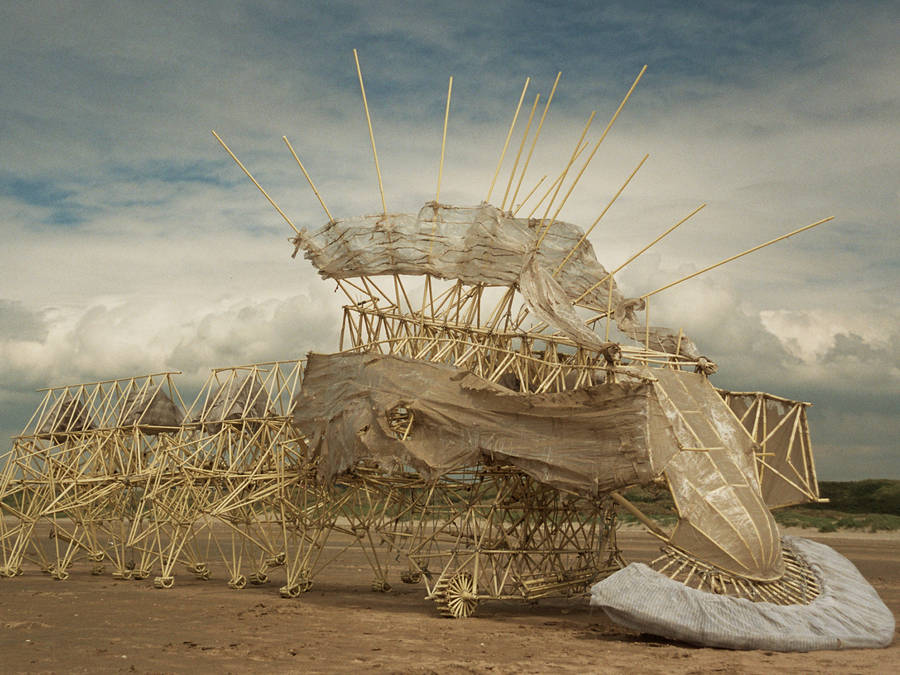
\includegraphics[width=0.9\linewidth]{figures/strandbeest}
	\captionof{figure}{One of Jansen's Strandbeests}
   	\label{strandbeest}
\end{figure}

\begin{figure}[h]
	\centering
	\begin{minipage}[b]{.8\textwidth}
		\centering
		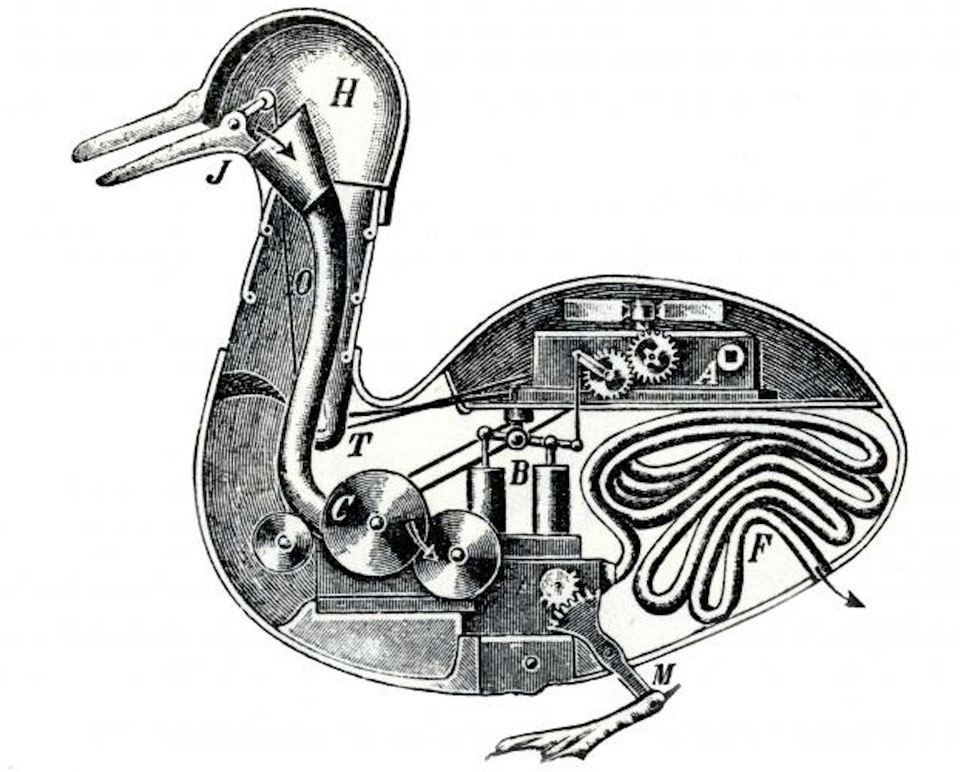
\includegraphics[width=.7\linewidth]{figures/vaucanson_duck}
		\captionof{figure}{A nineteenth-century inventor's imagined depiction of the inner workings of the Vaucanson Duck \citep{riskin2003defecating}}
		\label{vaucanson_duck}
	\end{minipage}
\end{figure}

These two examples, each impressive in their own right, points to the powerful expressiveness that actuation can give objects, as we have a tendency to relate things that move to living entities. 
\blank  
Looking back at traditional computing systems, before the era of Ubiquitous Computing \citep{weiser1991computer}, there has been a strong separation between the digital bits and the material world surrounding us.
The tangibility of digital information was then, for the most part, limited to keyboards and mice, icons and windows. 
And even though metaphors and graphical representations has helped us visualise the digital matter that flow through the transistors, these digital bits, when presented to the physical world, still only manifests as pixels on a screen, intangible and transient. 
\citet{ishii1997tangible} vision of Tangible Bits, along with Weiser's ubiquitous computing, was a break away from the traditions, where the goal was to create a strong coupling from the digital bits of the computer to the physical environments we surround ourself with.

The intangible and transient nature of digital bits is also one of the powerful aspects of such interfaces as this gives them a degree of malleability and adaptability that are not found in the physical objects.
This degree of malleability is not found in the in the physical objects that we surrounds us with, making a complete fusion of the digital and the physical world hard to achieve.
\blank
In 1965, Ivan Sutherland presented a vision of what he called the Ultimate Display \citep{sutherland1965ultimate}, envisioning a room where digital bits would control the existence of matter, completely removing the boundaries between the two worlds.
This display would attain the palpability of the physical world as well as the transience of the digital, as it would let digital information manifest itself into physical objects.
So a digital chair shown in this room would be good enough to sit in.

This is, of course, still only a vision, but in recent years there has been an increasing interest in bridging the gaps that still exists between the two worlds, such as physical malleability and transience.
Under different names such as kinetic interaction, organic user interfaces, actuated interfaces, shape-changing interfaces and programmable matter, researchers has attempted to get closer to creating truly ubiquitous systems.    
This has resulted in an increasing amount of of what \citet{coelho2009programming} calls `transient materials', such as flexible displays, shape-changing materials, e-textiles and sensor networks.
\blank
Interestingly some of these transient materials, especially e-textiles, have given rise to DIY communities that combines traditional crafts with electronics, inviting to a new form of material end-user-programming.
For example \citet{buechley2008lilypad}'s LilyPad Arduino which serves as a tool-kit for creating e-textile projects, Makey Makey\footnote{http://www.makeymakey.com/}, a tool-kit for tangible interaction, along with web communities such as Instructables\footnote{http://www.instructables.com/} and Make:\footnote{http://makezine.com/}.
DIY is interesting as a concept as it challenges the traditional balance between products and users making it possible for the consumer to create  or modify what he/she wants, instead of relying on the producer or designer to define what is wanted.
The DIY approach does somewhat democratise the product development as users are able to redefine or refit products to their needs, an approach that is also seen in the digital world with open-source software.
\blank
The idea of giving the control back to the user does also relate to the relationship between computers and user.
One of the areas of ubiquitous computing that have received a lot of focus is context-awareness.
First coined by \citet{schilit1994context}, context-aware computing focuses on letting the computer act based on contextual information.
But there is a tendency to exclude the user from the control-loop, as interaction possibilities, user intentions and actions are inferred from the sensed context, a context which might not correlate with what the user finds as the \emph{correct} one.
Implicit interaction is not necessarily a bad thing as it is the basis for many useful applications, especially in mobile computing, but we do believe that there is value in keeping the user in some degree of control
\blank
A domain where we find the relationship between computers and user interesting is the domestic environment.
An essential aspect of a home is the ability to make it one, in the sense that you, as an inhabitant, is able to modify it continuously to respond to your needs and desires as to what you want from your home.
As computers become an increasingly more integrated part of our everyday life, computers also have to be taken into account when we talk about the home.

Since the entrance of the personal computer into the home in the 80s much has happened.
Today we see deeply integrated `smart homes' where, in the extreme cases, even small changes to the house needs a call to a computer technician.
In a study of very wealthy people's smart homes, \citet{lynggaard2012had} mention that several of their informants had personal programmers just to configure and maintain their house.

The question is how to make computing systems in the home that are made to evolve and adapt and that functions on the premises of the inhabitants? This is part of of what we want to investigate further in this thesis.  
\blank
In this chapter we have tried to expose the inspirational background that has framed our thinking and our work on this thesis. 
We have introduced an array of areas that we seek inspiration from and will use to varying degrees, that is

\begin{itemize}
\item{The animation of inanimate objects}
\item{Ubiquitous computing and tangible interfaces}
\item{Transient materials and shape change in interfaces}
\item{Empowerment of the user, redefining the relationship between the user and the user interface}
\item{The home as a space for smart interaction}
\end{itemize}

In the midst of all these seemingly divergent digressions we believe that there is an unexplored space for interfaces that focuses on adaptability and situational awareness, that function on the terms of the user and not the computer system, bringing a more dynamic relationship, as seen in software, into the world of physical interactable artefacts.

Our thesis tries to shed light on a concept of Ad Hoc Interfaces, a concept that we want to explore and expand upon throughout this thesis and a concept that has evolved and taken inspiration from all of the above mentioned areas, and more. 
It is our goal to present a novel approach to making computing systems that are adaptable, modifiable and highly dynamic, while keeping the focus on the user. 

\section{Process}
\label{ch:intro/process}
%!TEX root = ../thesis.tex
Process is fun

\begin{verbatim}
related work will be presented throughout this thesis where relevant
\end{verbatim}



\section{Contribution}
\label{ch:intro/contri}
%!TEX root = ../thesis.tex
Contributions are fun

\begin{verbatim}
* AHI as a field/approach/way of thinking designerly
* Guidelines from lessons learned/evaluation/prototyping
\end{verbatim}

\newpage

\section{Thesis overview}
\label{ch:intro/overview}
%!TEX root = ../thesis.tex
We have chosen not to include a separate related work chapter in this thesis and related work will therefore be presented and related to throughout the thesis.
It is our hope that this will enable us to make the related work more relevant and context specific and therefore support our points better. 
\blank
\textbf{Chapter 1} is an introductory chapter where we give an overview of the domain of this thesis as well as a motivation for our work and the ideas that has inspired us.
\blank
\textbf{Chapter 2} gives an overview of the evolution of computers and their interfaces.
This overview enables us to situate ourself in a broader context of computer science and point to an area that we see possibilities in.  
\blank
\textbf{Chapter 3} is a discussion about the domestic environment as a domain and is used to provide a context for our design exploreaions. 
\blank
\textbf{Chapter 4} presents our initial notion of Ad Hoc Interfaces (AHIs) as a novel approach to interface design.
Here we present and situate AHIs in relation to existing literature and tendencies that were presented in chapter \ref{ch:ui} and \ref{ch:domain}, and in relation to existing designs that show ad hoc qualities.
We also envision three different approaches to constructing AHIs that we will explore in chapter \ref{ch:jamming}-\ref{ch:proto3}.
\blank
\textbf{Chapter 5} explores the design space of AHIs in the domestic environment through workshops conducted in the home.
\blank
\textbf{Chapter 6} explores the first approach to constructing AHIs. 
We describe our first prototype work that explores and surveys the possibility of creating AHIs based on shape-change and jamming techniques and present various concepts based on this.
\blank
\textbf{Chapter 7} describes and discusses the secondary construction approach where we, though several iterations of a prototype, explores the possibilities of creating embedded AHIs through electronic textiles.
\blank
\textbf{Chapter 8} explores the third approach where interfaces are constructed on the spot.
We discuss the approach based on concept designs and exploratory prototypes. 
Of the three approaches this is the most cursory.
\blank
\textbf{Chapter 9} zooms out from the specific design and concept explorations and returns to our notion of Ad Hoc Interfaces.
Our initial presentation of AHIs was mostly theory-driven, but we now complements it with a more \emph{research through design} oriented approach based on chapters \ref{ch:workshops}-\ref{ch:proto3}. 
\blank
\textbf{Chapter 10} concludes our thesis by both looking backwards to what we have achieved and contributed with, but also with a look forward, pointing to future work and directions that AHIs could benefit from.

\chapter{User Interfaces}
\label{ch:ui}
%!TEX root = thesis.tex
As a way of introduction we will here give an overview of the evolution of computer interfaces and how they have interacted and integrated with the users using them.
We will use this a starting point as to situate ourself in relation to the various fields of research in computer science and as a pointer to the future prospects of user interfaces, both in terms of what visions other researchers have proposed, and in relation to our own proposition for ad hoc interfaces.
We will first give a historical look back in time based on \citet{grudin1990computer}, from the early computers to the 1990s, which will both give an insight as to how the relationship between the user and computers has evolved, as well as point to a paradigm shift away from the terminal based computer.
We will follow this paradigm shift to the vision of ubiquitous computer, presented by \citet{weiser1991computer}, and look at some of the relevant related research area that has followed this vision.
Lastly we will point to an area where we see unused potential for future work, an area that throughout this thesis will be further articulated and conceptualized.   

\section{The computer reaches out}
There is of course many ways to look at the evolution of the computer and the user interface, and although it is hard to draw a straight line as to how the development has occurred, as much of the developments has happened in parallel, we try to outline the broad picture and give a pointer to the future.
As a start we have chosen to take an offset in \citeauthor{grudin1990computer}'s article about the historical continuity of interface design \citep{grudin1990computer} and along with that, the type of interaction that has been defining for each of \citeauthor{grudin1990computer}'s levels.

\citeauthor{grudin1990computer} describes the evolution of the user interface from the 1950's to the 1990's though five overall development foci or 'levels' for researchers, along with the principle user group for each level.
The five levels can be seen visualized in figure~\ref{foci-interface}.

\begin{figure}[hb]
	\centering
  		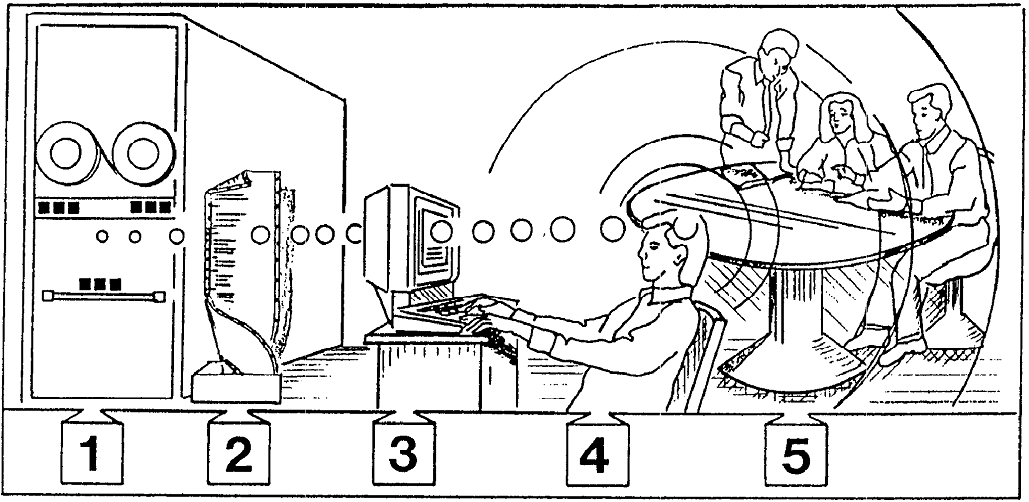
\includegraphics[width=3in]{figures/foci-interface}
	\caption[The development of user interfaces \citep{grudin1990computer}.]
   {The development of user interfaces, from \citep{grudin1990computer}.}
   \label{foci-interface}
\end{figure}
The levels should not be seen as isolated entities, as there exists interdependencies between the levels, for example before progress can be made to level 2, there might have to be made improvements to the hardware at level 1.

\subsubsection{Level 1: Interface as hardware}
At the first level (-1950s) the interface is seen as hardware, understood in the way that the interaction between the user and the computer is defined by the workings of the hardware.
So for engineers and programmers, which are the principal users, a central part of the user interaction involves the inner workings of the hardware.
A common way to interact at the time were, besides modifying the hardware, was though punch cards.
Punch cards represents digital information by the presence or absence of holes on the card, based on a predefined pattern which the computer can then read.
The user would use a machine to punch holes in the cards which could contain programming commands or it could be used as an analogue data storage that could later be read by the computer.
From a human perspective the interaction at the time was very much on the premises of the computer, as the language of interaction was based on things like binary numbers, hexadecimals and memory locations.

\subsubsection{Level 2: Interface as software}
The second level (1960s-1970s) defines the interface as software.
As the hardware level is abstracted away by advancements in software and programming languages programmers and the interface they interacts with moves away from the physical inner workings of the computer and onto software.
The main users now mostly programmers and the interface focus is on the computer, so the user interaction is still on the premises of the computer, with a lack of attention to human factors like legibility of code.
Programmers interacted with the computer though assembly code, compilers and mathematics as the main focus of the computer was on computations. The notion of a \emph{user interface} was still unarticulated as interface development was focused on programmer efficiency, not human factors.

\subsubsection{Level 3: Interface as terminal}
At the third level (1970s-1990s) the interface focus moves away from the programming task and onto the terminal where the dominant user is no longer necessarily programmers or engineers, but seen more broadly as \emph{end-users}.
Grundin also marks this as the start of the discipline of human-computer interaction, including the `human' in the computer interaction.
The move to the terminals was made possible by advances in visual displays and interactive capabilities, letting the user, to a larger degree than before, interact on more human terms where the interface aids the user in the interaction.

With the emergence of the computer mice and more powerful computers, Graphical User Interfaces (GUIs) became, and still is, the most popular method of interacting with the computer.
One of the main aspects of the GUI is the use of visual metaphors, inspired by the real world, to guide the users actions and understanding of the system.
The most well knows being the desktop metaphor that links the office space to the computer with digital folders, documents, trash bins and so on, simulating a physical desktop on the monitor.
The central components of the desktop metaphor being windows, icons, menus and pointers, also known as the WIMP paradigm \citep[chap. 6]{krumm2009ubiquitous}. 
Using metaphors in this way can ease the user's annexation into the digital world as they, if done properly, creates logical links between knows physical actions and potential digital actions.

\subsubsection{Level 4: Interface as dialogue}
The use of metaphors as described in level 3 does also somewhat fit into the this level since the GUI, in the previous example, is adapting physical attributes (the office) into the virtual space and in that way incorporates the surrounding environment, though in a static way.
The fourth level (1980s-) focus on the interface as an interaction dialogue where the interface can be adapted and tailored, by the computer, to the specific user.
This could for example be computer systems, over time, gathers information about the users interaction patterns enabling it to possibly foresee a user action, and maybe by making it easier to execute the action, assisting the user.
Grundin sees it as the computer \emph{``is extending its grasp beyond the keyboard and the display surface''} in the sense that the computer now has some knowledge about the user which lets it partake in a two-way dialogue.

\subsubsection{Level 5: Interface as work setting}
The fifth level (1990s-) takes the interaction dialogue to the work or social setting, moving the interface further away from the computer.
The principal user is now a group of ``end-users'' and as the interaction takes place in a social setting it is increasingly necessary for the computer to have information about the surrounding environment.
Social settings are generally complex structures where environment, culture, social structures, group dynamics, and context all play a role in the dynamics of social interaction.
All of these aspects needs, to some degree, to be design for in a user interface aimed at the work or social setting, increasing the complexity of the system.
\blank
Grundins five levels describes a movement where the interface separates itself from the physical enclosure of the hardware and into the cognitive and social structures of humans.
\citeauthor{grudin1990computer} himself describes it as a continuously \emph{``outward movement of the computer's interface to its external environment''}.
A concequence of this is that a move in the interaction language also happens, from abstract to natural, in terms of the human readability, as the focus of the interface moves from the computer to its user.

Grundin points out that as of 1990 most work has been focused on the third level but he sees a future where the interface dialogue and the social setting is increasingly influential in the design of computing systems.
This notion is not far away from what \citeauthor{weiser1991computer} presents a year later in his vision of ubiquitous computing \citep{weiser1991computer}.

\subsection{Ubiquitous computing}
In traditional computer systems there has generally been a strong separation between the physical and the digital, but with ubiquitous computing, not only does the computer's interface move to its external environment, as Grundin pointed to, we also see that the computer itself moves into the environment, creating a stronger link between the physical world and the digital world.
A consequence of ubiquitous computing is also a change in the relationship between the user and computers.
This change can be seen by looking at the evolution of the relationship, which can be roughly split into three generations or eras \citep{weiser1997coming,abowd2012next}.
\begin{itemize}
\item[] \textbf{1\textsuperscript{st} generation} being terminal based computing where multiple users share the same computer in a many-to-one relationship.
\item[] \textbf{2\textsuperscript{nd} generation} where the personal computing revolution happens and it becomes possible to have \emph{your} computer, in a one-to-one relationship between the computer and the user.
\item[] \textbf{3\textsuperscript{rd} generation} being ubiquitous computing, here a one-to-many relationship becomes possible as computers move out into the world and multiple computers now shares and interacts with a single person.
\end{itemize}

The idea of ubiquitous computing, as presented in \citep{weiser1991computer}, is that a multitude of interconnected computers are embedded seamlessly into the environment as to become invisible, both physical and metaphorical, and integrate into the everyday life of people.
In contrast to terminal based computing, interactions with these systems can happen everywhere, with a multitude of different devices with computers with many different forms. 
This points to two key aspects of attaining this vision, \emph{location} and \emph{scale}.
The purpose of location is to be able to inform the user and adapt to the need of the user based on the location context available to system. 
The aspect of scale is relevant for creating \emph{``machines that fit the human environment, instead of
forcing humans to enter their''}, as \citeauthor{weiser1991computer} puts it, where different sized computers can fit into different environments, contexts or functions. 

This vision of moving a multitude of computers and their user interface out into the world has been the basis inspiration for an array of related research areas, each with a specific focus or approach, but with the shared purpose of going beyond the situated use of the desktop computer, and its WIMP interface, and move into the environment.

We will limit ourself to present only a selected few areas following the ubiquitous vision that we find relevant to our own work and which will be further discussed throughout the thesis.
\subsubsection{Context Awareness (CA)}
As mentioned a key part of ubiquitous computing is location and this has laid the basis for the research area of context awareness.
There has been many definition of context and context aware computing, the first being by \citet{schilit1994context}, but here we will stick to the definition proposed by \citeauthor{abowd1999towards} as we find it more encompassing. 

\citet{abowd1999towards} defines context-aware computing as \emph{``the use of context to
provide task-relevant information and/or services to a user''}, where context is \emph{``any information that can be used characterize the situation of an entity''} and entity describing anything that is relevant for the application or user.
\citeauthor{abowd1999towards} describe the control loop of CA applications as three-parted. 
First the application looks at the incoming context, this is the \emph{who's, where's, when's and what's} and based on this information decides on a \emph{why} the situation is occurring and when the \emph{why} is decided, the application should act accordingly with an appropriate \emph{action}
One of the main challenges of making such systems is to define which parts of the context that is relevant in a given situation and how it should translate into a \emph{why}, as this is something that the application designer as to encode into the application.

\subsubsection{Tangible User Interfaces (TUI)}
TUIs attempts to create physical representations of the digital state of the computer, embedding a digital layer into physical objects and environments.
The term was first coined by \citet{ishii1997tangible}, building on Weiser's vision of the ubiquitous and invisible computer.
Ishii and Ullmer states two goals for TUIs:
\begin{itemize}
    \item{allowing users to ``grasp and manipulate'' foreground bits by coupling bits with physical objects, and}
    \item{enabling users to be aware of background bits at the periphery using ambient media in an augmented space}
\end{itemize}
By embodying digital information into tangible objects, TUI systems takes advantage of humans ability to sense, interact and manipulate the physical world. 


\section{A possible future for user interfaces}
\todo{not done at all}
As Abowd correctly notes, Weiser's vision has to some extend become reality. 
Computers are part of the environment and have indeed been \textit{woven} into the fabric of everyday life in many ways. \todo{giv nogle simple eksempler} 
If we are beginning to pass the 3\textsuperscript{rd}, Abowd asks \textit{so, what's next?}.
This is of course a complex and difficult question to answer.
Abowd suggests a future where the human-computer experience is more conjoined than ever, blurring the boundaries between them.
\begin{quote}
\emph{[\ldots] our own physical being and our sense of identity is no longer easily distinguished from elements of computing.}
\end{quote}
Abowd also touches on a topic that has been dominant in the last few years, namely cloud computing.
Broadly seen cloud computing refers to services and applications that are made available over a network \todo{wiki ref?}.
This could be data storage, computing power, back-up services or applications which makes traditional desktop applications available through the Internet.
Abowd suggests that future devices will be able to adapt to whoever is currently using it, as all relevant information will available be in from the cloud.
Following this, devices and their services no longer have to be closely ties together, leading the way for genetic multi purpose devices that delivers services from the cloud.

\citet{ishii2012radical} presents an alternative vision for the future.
They presents the vision as \textit{Radical Atoms}, a vision for the future of \textit{human-material interaction} or \textit{material user interface}. 

\todo{noget med shape change - ledende op til SC afsnit og vores protype og ide om ad hoc interfaces}
\todo{3.wave HCI bødker}

\chapter{Domain}
\label{ch:domain}
%!TEX root = thesis.tex
As we noted in the introduction, the domestic environment is a domain where we find the relationship between computers and user interesting.
The domestic environment is interesting because we see the home as a space where adaptability, personalization, and ??  are central aspects of making a home \emph{home} and as such our idea of AHI, that we will present in chapter~\ref{ch:adhoc}, feels appropriate and relevant in this domain.
We have chosen this as a design constraint with the hope it will enable us to make a more precise and sharp presentation and exploration of the possibilities of AHIs as we are now forced to put it into a specific context.

As a point of origin we will first look at the building as a concept and how the building relates to changes and to the people that inhabits its walls.
Secondly we will look into so called ``smart homes'', homes where computers becomes large part of the ecology of the home, as this poses interesting possibilities and challenges for designing computer systems.

\section{The evolution of buildings}
Buildings, like everything else, changes over time.
But different parts of a building change with different rates, a wall will most likely endure longer than the paint on its sides and the ground on which the wall stands will most likely still be there when the wall collapses.
This ever changing nature of buildings has been conceptualized by Steward Brand in his book \emph{How Buildings Learn: What Happens After They're Built} \citep{brand1995buildings}.
Here Brand presents a framework, in which he define six S's as a ground for understanding changes in a building: Site, Structure, Skin, Services, Space plan and Stuff.

\begin{figure}[h]
	\centering
  		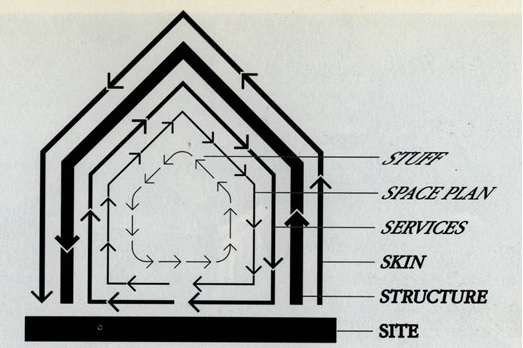
\includegraphics[width=3.5in]{figures/brand-diagram}
	\caption{The different layers of change \citep[chapter 2]{brand1995buildings}}
   \label{brand-diagram}
\end{figure}

The six S's describes the different layers of change, three describing the exterior: Site, Structure and Skin and three describing the interior: Services, Space plan and Stuff.
Each layer has a different rate of change, Site having the longest and Stuff the shortest rate of change, see figure~\ref{brand-diagram}.
As the rate of change differs for the different components of the building, the building is, as Brand notes, constantly `tearing itself apart', or in a more constructive term, constantly evolving.

Brand argues in favor for an approach where the inhabitants of a building can evolve and change the building over time according to their needs \citep{brandBBCvideo}.
He sees this in contrast to a scenario where a single person or group designs a building for others to use.
In light of this, providing inhabitants with higher rates of change could accommodate an even more dynamic relationship between the building and the people living in it.

We see two interesting ways of exploring this existing relationship between building and inhabitants.
One is to open up the layer of Stuff.
The layer of Stuff is all the things that gets moved around or changed on daily to monthly basis such as chairs and desks, kitchen appliances and lamps.
So what if Stuff could be changed, moved or modified on an even more frequent basis, say in minutes or hours, accommodating the need of the inhabitants with the possibility for them to adapt furniture and objects to current needs.

Another approach could be to pull down a given layer of change to a lower layer, for example enabling changes in the Space Plan as if it was Stuff, creating a more dynamic Space Plan.
This would open up for entirely new possibilities of rethinking the home. 
If, for example, homes had dynamic walls, ceilings, floors and doors that would give them a less static and permanent function, it could enable changes to the Space Plan that maybe lasts days or months, enabling the Space Plan to adapt to specific situations, just as you on the Stuff plan would add an extra chair to the table for a visiting guest. 

It is, of course, non trivial to make the home as dynamic and adaptable as suggested above.
But the this concept of the building as a living, ever-evolving entity, does give us inspiration to explore the use of digital systems in a domestic setting, as this could be one way to approach such a vision.
So with the help of computers and new materials we want to explore how we can accommodate and design for change in physical environment that surrounds us.
We want to explore how physical interfaces can be created on demand in an ad hoc manner, to better cope with the changes in the buildings space plan and on the level of stuff, and better accommodate the changing needs of its inhabitants.
As touched upon in chapter~\ref{ch:ui} this does somewhat challenge the traditional view of physical interfaces as they are generally considered static and permanent.
\todo{bedre afrunding til smart homes}
hvad skal der komme ud af det

Smart homes - ideen om det teknologiske hus
intro
definition/vision
complex setting
rodden - hvem skal deltage 

\section{Smart homes or home that make us smart}
\todo{section not done - needs work}

The idea of adding computer systems into the domestic environment is not a new one.
Ever since the emergence of electricity into the households, electrical appliances has been a part of the domestic setting.
And along with the increasingly more advanced appliances being developed, the dream and vision of even more sophisticated systems have continuously evolved

An early visual example of the fascination of `smart homes' is seen in the General Motors commercial film \emph{Design for Dreaming}\footnote{http://en.wikipedia.org/wiki/Design\_for\_Dreaming} from 1956 \citep{designfordreaming}, where the \emph{Home of the Future}\footnote{http://en.wikipedia.org/wiki/Home\_of\_the\_future} is presented.
Here we see a remote control of the different kitchen appliances, a (computer)screen that can show the final result of the recipe it is given, and a seemingly context-aware moving table.
Domestic technology appears even earlier where in the 1915-20, with the advent of electricity in common homes, electrically powered machines such as vacuum cleaners and refrigerators providing the `seedbed', as \citet{aldrich2003smart} puts it, for the emergence of the smart home.

In recent years, especially since Mark Weiser's vision of ubiquitous computing \citep{weiser1991computer}, a lot of the research in the domestic realm has focused on the idea of a \emph{home that is smart} where the goal is to use computers to make the home \emph{intelligent} \citep{taylor2007homes}.
\citet{aldrich2003smart} defines smart homes as:

\begin{quotation}
\emph{A ``smart home'' can be defined as a residence equipped with computing and information technology which anticipates and responds to the needs of the occupants, working to promote their comfort, convenience, security and entertainment through the management of technology within the home and connections to the world beyond.}
\end{quotation}
\citeauthor{aldrich2003smart} sees this definition as the acme of domestic technology as we can envision it today, putting it somewhere in between reality and fantasy.
\todo{mere her}

The domestic setting differs a lot from the traditional office setting where most research on ubiquitous computing has been conducted, and is in some ways even more complex as people in the domestic setting has a lot more freedom as to how they organize their space and time \cite{meyer2003survey}.
Also the aspect of user experience needs special consideration when introducing new technology to the home, whereas in a work setting the user might \emph{need} to use the new technology, imposed upon him by superiors, the technology for the home need to be usable and useful enough so that the user \emph{wants} to use \citep{meyer2003survey}.
\todo{maaske undlade naeste del}
A thorough look at the challenges related to creating ubiquitous computing for the home is presented by \citet{edwards2001home}.
Here Edwards et al. identifies seven challenges that need to be overcome before the vision of the ubiquitous smart home can become a reality. We will return to these challenges in relation to our own prototypes \todo{ref til prototype sektion}.

\citet{rodden2003evolution} have built upon Brands framework in the context of ubiquitous computing and the domestic setting and is therefore relevant for us here.
By looking at existing research Rodden et al. identifies three main approaches for creating interactive devices for domestic settings.

\begin{itemize}
  \item \emph{Information Appliance} that are stand-alone, self-contained devices that are often used as a layer of interactive functions on top of an existing appliance.
  \item \emph{Interactive Household Objects} that embeds interactive capabilities into existing household objects to create new means of interaction and communication, often building upon the existing understanding and metaphors associated with the household object.
  \item \emph{Augmented Furniture} that embeds sensory systems into furniture to add interactive capabilities. \ldots
\end{itemize}

Rodden et al. notes that the technology is most intrusive in information appliances, less so in interactive household objects and least in augmented furniture.

\todo{noget om bygninger ikke er nybyggerier og noget mere Rodden}
 
\todo{diskussion om empoverment, Brand/Rodden vs smart-homes/context-awareness/dubai-huse}

\todo{make systems that are not dictated by a designer, but made for adaptation and modification. People are different and have different, changing, needs. Systems needs to repsond to this}


\chapter{Ad Hoc Interfaces}
\label{ch:adhoc}
%!TEX root = thesis.tex

In this thesis we will introduce the notion of \emph{ad hoc interfaces} or AHIs.

Being \emph{ad hoc} generelly means something made for a specific task or creating meaning in changing contexts.
The word itself originates from the Latin language and literally means \emph{for this} (situation). 
In modern english the two word combination is regarded as a single word and the Oxford Dictionary\footnote{http://oxforddictionaries.com/definition/english/ad-hoc} defines it as

\begin{quotation}
\textbf{Ad hoc}  /ad 'h\textturnscripta k/

created or done for a particular purpose as necessary
\end{quotation}

The word is used in many different fields and context.
For example, In society committees a formed on an ad hoc basis to deal with specific tasks, investigations or analyses.

In computer science wireless networking can be of an ad hoc nature, which means that that the network is not dependent on a preexisting infrastructure.
Wireless ad hoc networks are highly dynamic and all participating nodes in the network graph are more or less doing routing for each other.
This makes the network adaptive to changing contexts, which is an important element of ubiquitous computing.

In general a user works with a computer in an ad hoc manner.
General purpose computers are very good at supporting ad hoc activities with their multitasking capabilities.
Applications are used when needed and maybe even used in connection with each other.
Windows are opened, closed and arranged as needed to support different use cases.

So, ad hoc is a prevalent characteristic within many activities and contexts.
Next we will give our own definition of being ad hoc when applied to the field of user interfaces and also compare this to other elements of \todo{computer science}.

\section{Defining ad hoc interfaces} 
We define ad hoc interfaces as 

\begin{quotation}\label{adhoc:definition}
\emph{physical interfaces that can be \todo{created} or accessed on} 

\emph{demand for a particular purpose in mind. }
\end{quotation}

In this sense there is a degree of temporality embedded in the definition, in that the interaction is somewhat impromptu and the purpose is non-continuing.
The interface can be accessed when needed and when the interaction and purpose has ended it ``disappears'' again.
This makes good sense in the digital realm as pixels on a screen can easily be controlled and abstracted to bring attention to different tasks.
The questions is, how do we apply these ad hoc elements or characteristics to physical interfaces.
The physical world comes with many constraints compared to the digital as we are limited by the characteristics of the materials we interact with and the general laws of physics.
We can't just magically make physical objects appear and disappear which is possible, and easy, to do on a digital display.

We see two overall approaches to creating physical interfaces with ad hoc capabilities \todo{Stefan sees two ways while writing this ;-)}.
\begin{itemize}
	\item{Through invisible interfaces embedded into the physical environment}
	\item{Using shape change as the construction mechanism}
\end{itemize}

The two approaches does not exclude each other as they could surely be combined while still living up to our definition.
In the following we will elaborate on each approach separately.

\subsubsection{Embedding invisible interfaces into the physical environment}

In this case an existing element of the environment will contain the interface.
An element can be both a physical object, for example walls, furniture, devices etc, and also ambient air \todo{there is a better word for this}.
The perceived action possibilities are constrained by the affordances of the object. 
The input and output possibilities depend on the materiality of the physical object.
A variety of sensors can be used for input and actuators for output.

In \autoref{ch:textile-touch} we explore this approach.

\subsubsection{Using shape change as the construction mechanism}

In this case an objects shape changing capabilities lets it shift or morph into an particular interface.
Affordances are here dictated by the perceived action possibilities of the particular end-shape.
Again, sensors and actuators can be embedded for input and output control.
``No longer does form follow function, form becomes function''

In \autoref{ch:jamming} we explore this approach.

\todo{But what can we do} 
\begin{verbatim}
create interface: shape-change tilgange
create i bogstavelig forstand: bare paint
access interface: textile-touch

introducerer muligheden for baade space- og time multiplexing
\end{verbatim}

Let's first have a look at some existing products and projects which we have found that exhibit ad hoc characteristics. \todo{\ensuremath{\leftarrow} overgang til naeste subsektion}

\subsection{Products with ad hoc characteristics}
Ad hoc characteristics in interfaces are not some novel invention and they an be found in several existing products.
A simple example would be The Clapper~(figure~\ref{ch:adhoc:theclapper})~\cite{theclapperWIKIPEDIA} from the mid eighties, an electrical switch reacting to sounds in a specific frequency, tuned to claps, to turn a switch on and off respectively.
Here the interface is pervasive in the nearby environment and one interacts with it when needed after which it ``disappears'' again.

\begin{figure}[hb]
	\centering
  		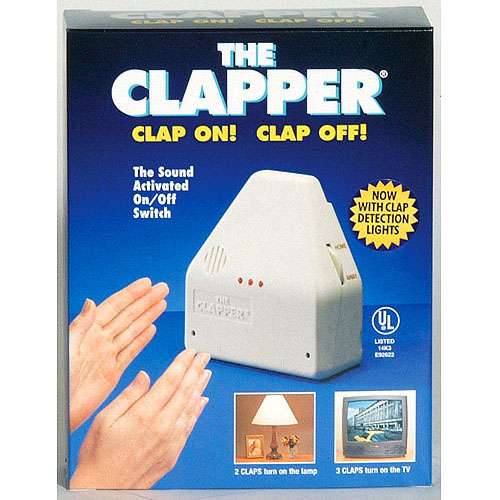
\includegraphics[width=1in]{figures/theclapper}
	\caption[The Clapper, a sound activated electronic switch.]
   {The Clapper, a sound activated electronic switch.}
   \label{ch:adhoc:theclapper}
\end{figure}

Another example is the conceptual and somewhat futuristic product ShapePhone (figure~\ref{fig:ch:jamming:jui-phone}) based on particle jamming, which will also be addressed in \autoref{ch:jamming}.
ShapePhone is generic shape changing product which changes it behaviour based on its physical form.
For example, in its base form it is a phone but when wrapped around a wrist it could serve as a watch and when folded in some other way it could be a game controller.
So, the different interfaces are created on demand by the user and have very different purposes of use depending on the form of the interface.

In a masters course in 2011 called Innovation Project \cite{innoproj2011, beomotionreportstefan, beomotionreporttore}  we, the authors, designed and implemented a dynamic shape shifting wall module with the ability to change its surface structure for acoustic regulation, i.e. diffusion, absorption and reflection for optimal conditions.
On top of that the module had illuminating features so that different areas could light up and serve as an aesthetic lighting for the atmosphere of the room.
The idea for the module was to retain the aesthetics of existing surroundings, so the module was not in use, the module would be `invisible' and flat like the wall.  
We envisioned two scenarios of use for the wall.
One where context awareness was the primary driver which meant that everything (acoustic and lighting conditions) would be automatically sensed and the wall module would modify itself accordingly and shift from flat to active.
In the other scenario the user would, to a higher degree, be in control.
The user could actively create deformations on the surface for aesthetic purposes and also control illuminated areas by interacting with the wall surface, see \ref{fig:ch:adhoc:beomotion}.
In this scenario the interface was shaped and created by the user for the specific situation, i.e. current acoustic and lightning conditions, as well as the desired aesthetic expression. 

\todo{afslut afrunding} And of course, also the inherent ad hoc nature of the way we interact with personal computers as mentioned in the introduction of this chapter.
\blank
\todo{2-3 flere eksempler \dots} 

\begin{figure}
	\centering
	\begin{subfigure}{.46\textwidth}
		\centering
		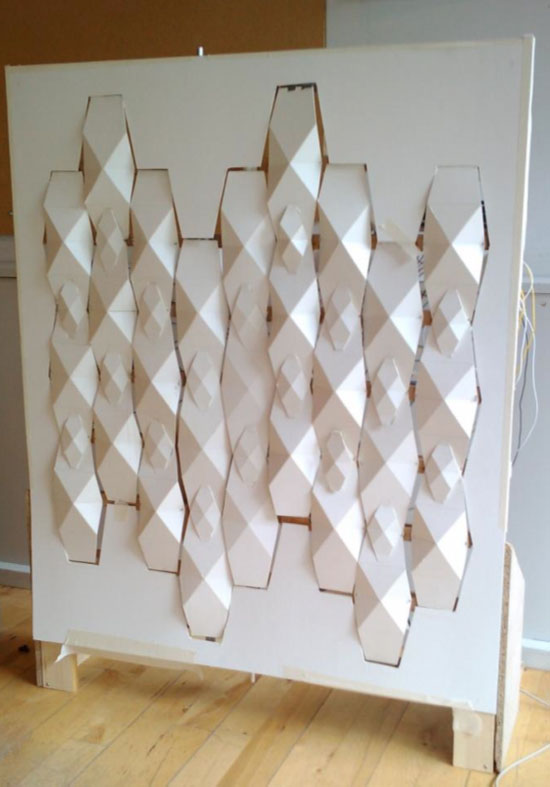
\includegraphics[width=.9\linewidth]{figures/beomotion/prototype}
		\caption{Interactive prototype}
	\end{subfigure}%
	\begin{subfigure}{.54\textwidth}
		\centering
		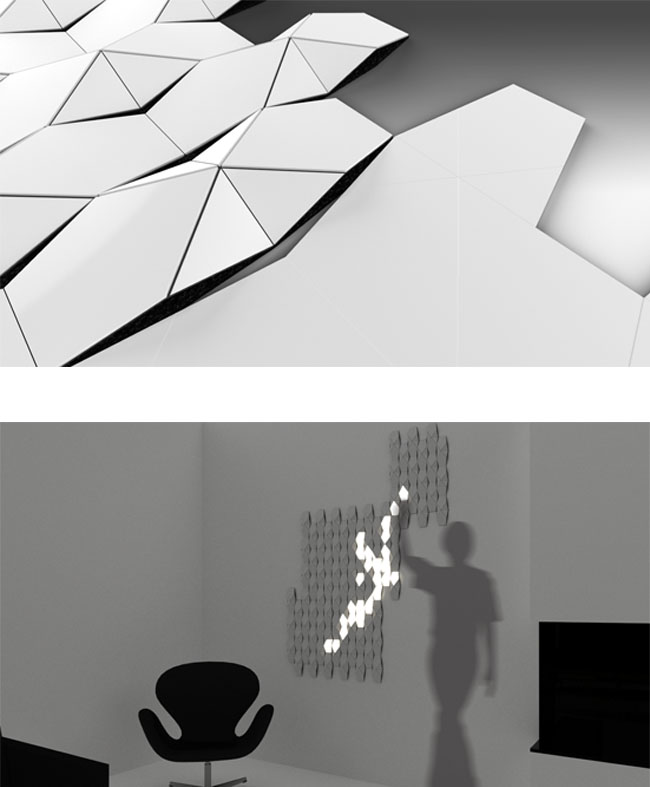
\includegraphics[width=.9\linewidth]{figures/beomotion/concepts}
		\caption{Concept illustrations}
	\end{subfigure}
	\caption{BeoMotion product design, Innovation Project, Aarhus University 2011}
	\label{fig:ch:adhoc:beomotion}
\end{figure}

\subsection{Relationship with other fields} 
% CAC comparison
It might seem that AHI overlaps with the concept of Context Aware Computing in that they both have a focus on environmental context.
In context aware computing a system attempts to derive, through a variety of cues, what the current context of use is and as a result it adapts its behaviour \citep[chap. 8]{krumm2009ubiquitous}. 
In this way it is the system itself that takes action autonomously and the user continues on outside of the control loop. \todo{rephrase??}
Exactly the topic of control is one of the points where context aware systems have received criticism \cite{erickson2002some}, \citep[chap. 8]{krumm2009ubiquitous}.
The criticism has to do with a systems ability to make inference based on the analysis of quantitative contextual information available, something that can be quite difficult to do for a computer as contextual information is often subtle and implicit.
\todo{This is not supposed to be a critique of context aware systems as they surely have their legitimacy and offer a lot of convenience.}
\todo{An AHI can have CAC elements} 

Where context aware systems put the user out of the control loop AHIs do not.
In AHIs the user is the initiator of action.

It actually makes no sense to compare them directly as they cannot be juxtaposed.
They are both elements or characteristics of a system and one does not exclude the other as a part of a system.
It would seem quite natural to have an ad hoc system that also incorporates some context aware computing elements, for example \todo{give a good example} 
\blank
% TUI comparison
Tangible user interfaces, or TUIs, do generally not exhibit ad hoc characteristics. \todo{det skal lige overvejes om det er helt sandt- NEJ}
They are mentioned here more for their nature of physical representation and their movement away from the standard GUI paradigm for human-computer interaction.
TUIs demonstrate a inherently tight coupling between digital information and the associated physical representation, for example tangible tokens representing a specific digital entity or mapping to a specific function or action.
There are numerous examples of these, for example, the ReacTable \cite{jorda2007reactable}, the Marble Answering Machine \todo{citation possible or link} to name a few.
Furthermore, because of this tight coupling the physical representations are often created only for the specific purpose and are of no use outside of the TUI context. \todo{er det at sk\ae re det over en kam??}

In contrast, ad hoc interfaces define a more loose coupling meaning that one physical object can serve several purposes. \todo{igen - ???}
This will be exemplified in \autoref{ch:textile-touch} where we prototype a general purpose ad hoc interface called textile touch, which can augment existing household objects by adding a digital layer.
\blank
\todo{and Augmented reality - While on the topic of adding a digital layer to the real-world environment we should also bring up the concept of Augmented Reality, or AR.}

\section{Discussion}

By giving an overview of related fields within HCI it is apparent that ad hoc interfaces relates in one way or another to other 

Opsumm\'er ad hoc
\begin{verbatim}
Ad hoc definiton
Some existing products exhibit ad hoc behaviour 
bringing together different aspects of various fields within HCI.

``fashioned from whatever is immediately available'' - may not quite be possible

Hvad aabner det op for.

\end{verbatim}

\chapter{User Studies}
\label{ch:workshops}
%!TEX root = thesis.tex
\todo{Change all names to fictional names}

Preliminary workshops were conducted to explore the design space of \todo{ad hoc interfaces} in the home environment.
The intend was to get a deeper understanding of how regular users, the participants, interact with products in their home and to explore the potential in the notion of \todo{ad hoc interfaces}.

\section{Workshop approach}

Our approach to the workshops was inspired by different elements from the literature. \todo{\dots}

We chose to conduct the workshops in the homes of the participants as it of course is a very familiar setting where the participants would \hl{be on top and not feel as guests ...}

\subsection{Fictional space}

\todo{what is fictional space}

When trying to explore though interactions and situations it can be beneficial to scope the setting by staging a concrete and limited scenario which participants can adhere to.

\todo{creating obstructions and staging the situation.}

\subsection{Inspiration cards}

illustrative cards on metaphores and technology.

\subsection{Props}

\todo{mangler bl.a. at bringe teori p\aa \ banen}

In preparation for the workshops we collected a variety of different props that could potentially be useful mediators during the workshops.
The intention here was to have artefacts that could spur imagination amongst the participants and help stage the fictional spaces created.

Figure~\ref{ch:workshops:props-box} shows a box with the props chosen for the workshops.

\begin{itemize}
  \item{Pen, paper(A3, A4), Post-Its, white board foil and transparencies for sketching, drawing and note-taking.}
  \item{Different fabrics like cloth and a fabric-surface mousepad for their flexible characteristics.}
  \item{Plasticine for direct manipulation and for moulding different shapes}
  \item{Rigid objects which could have imaginative behaviour and functionality.}
\end{itemize}

\begin{figure}[hb]
  \centering
    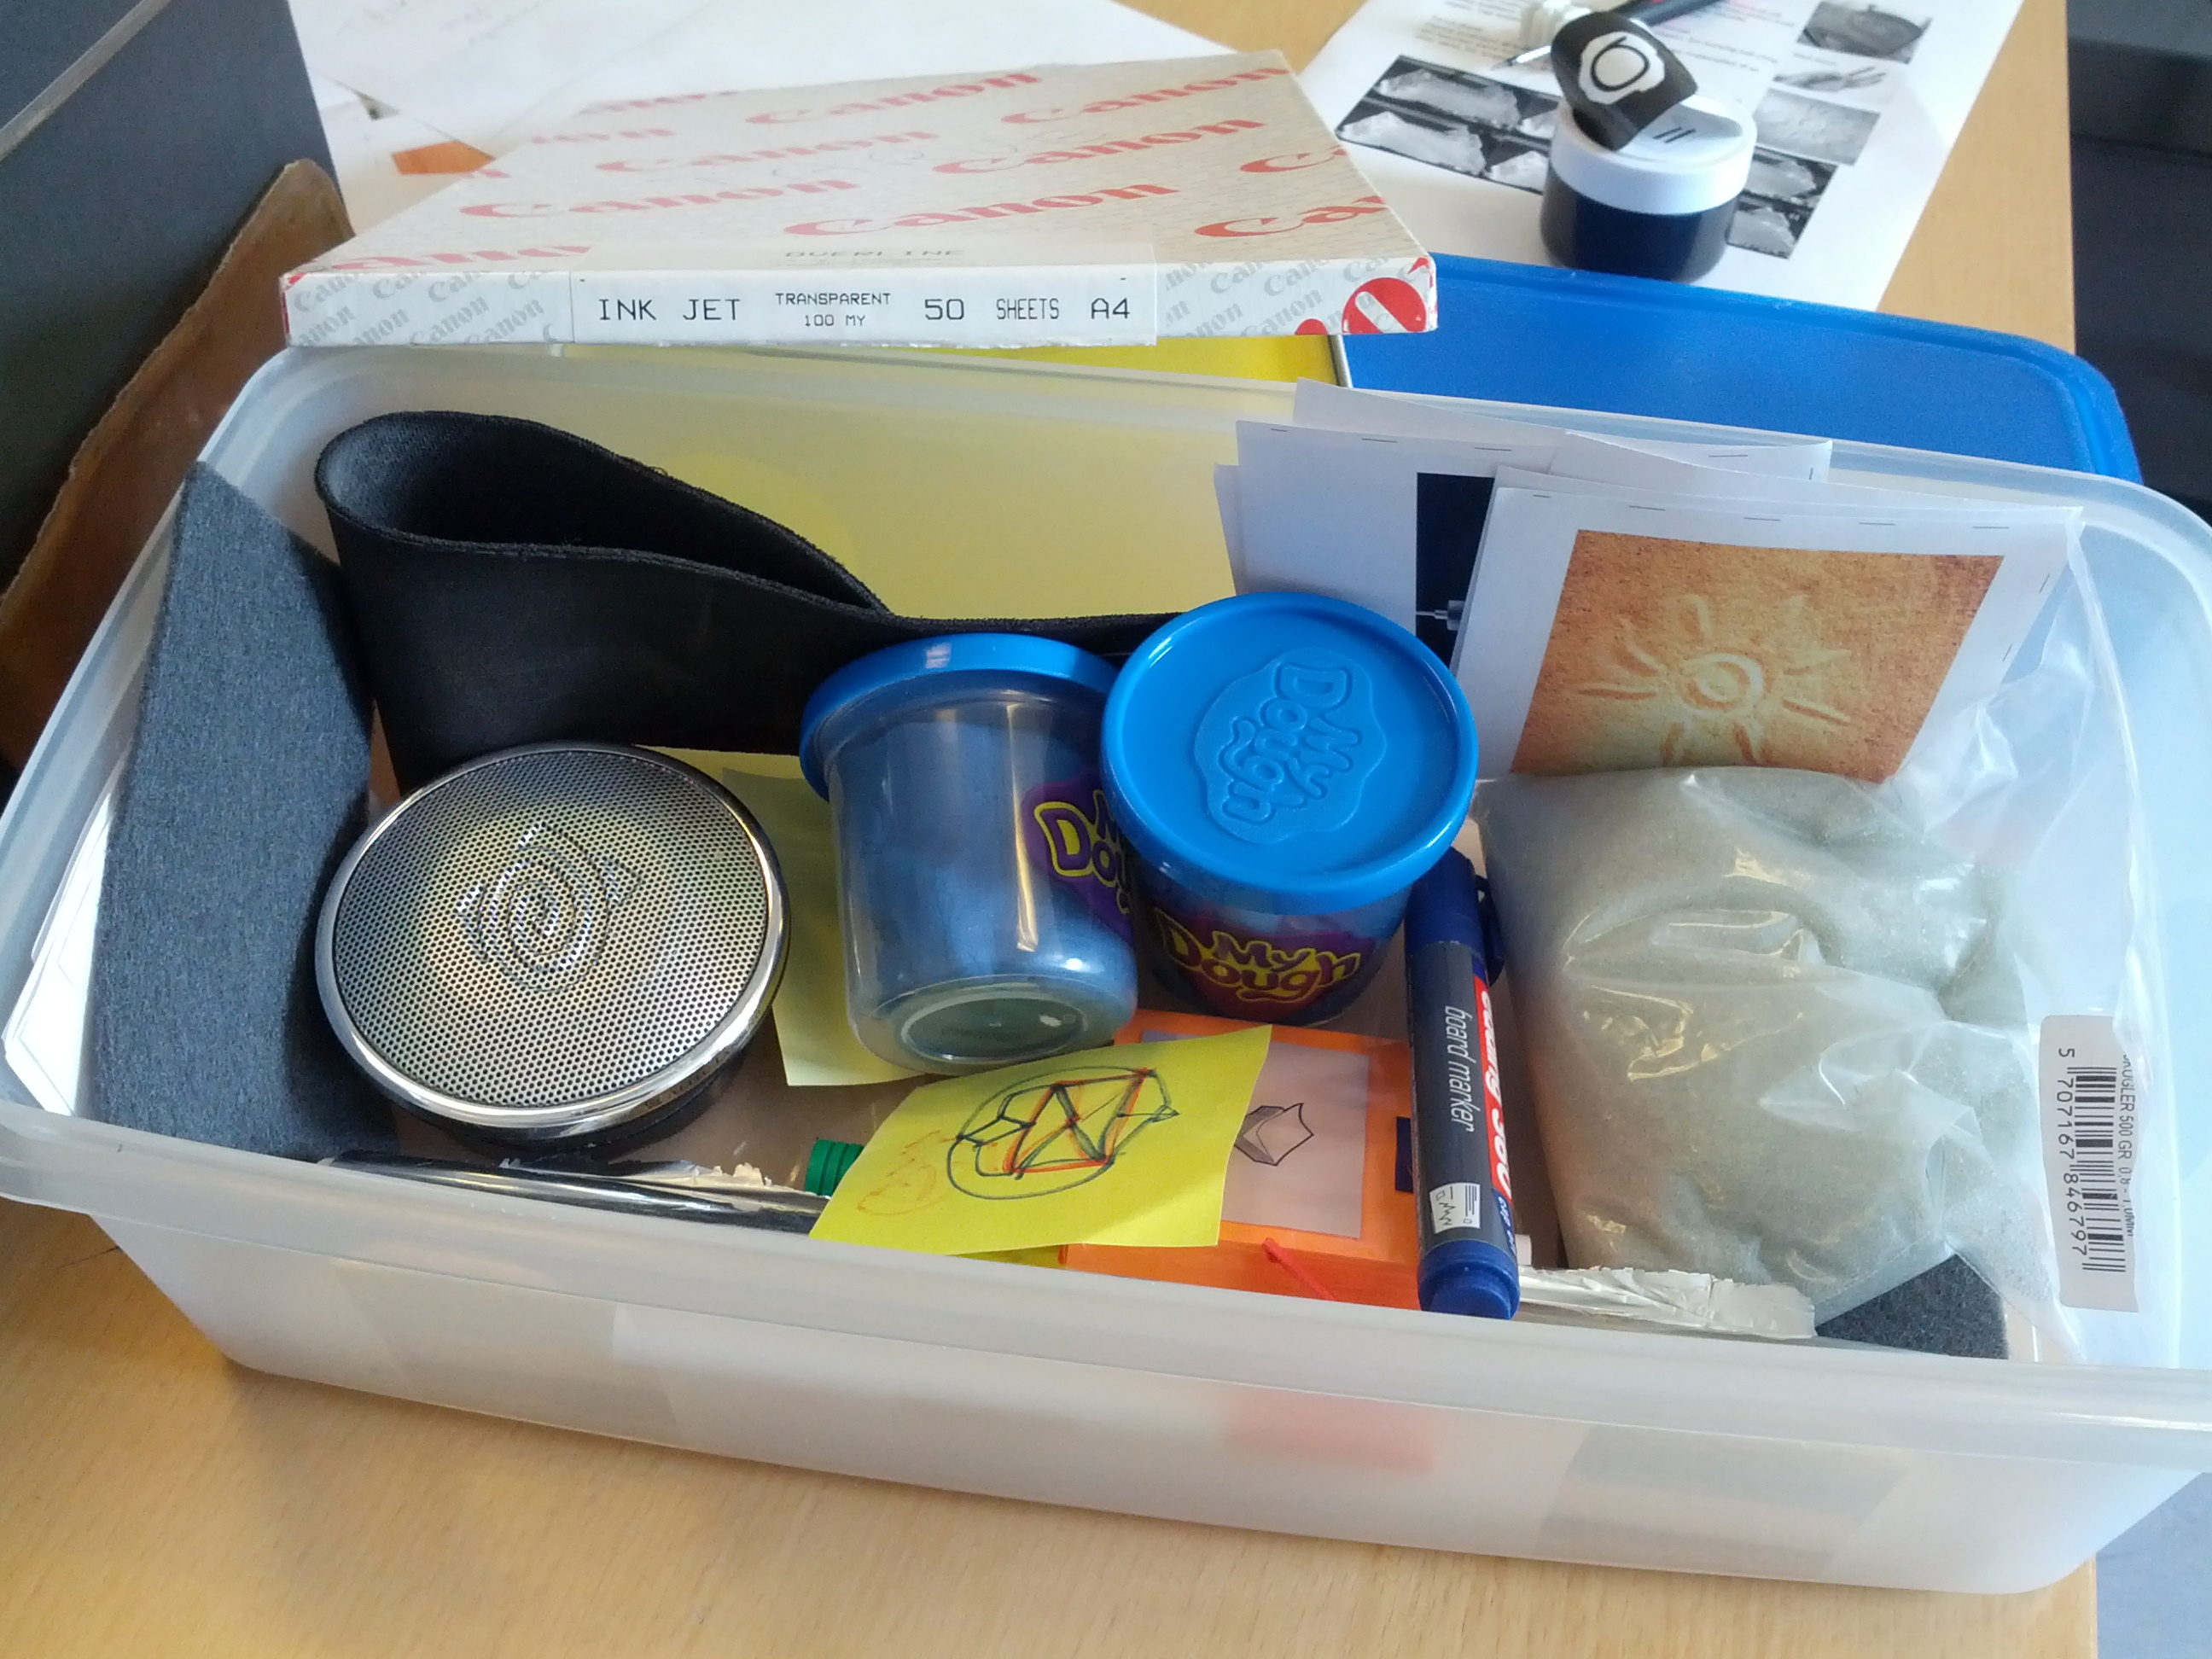
\includegraphics[width=4in]{workshops/props-box}
    \caption[A box with a variety of workshop props.] % in list of figures
  {The box with a variety of workshop props.} % beneath the figure
  \label{ch:workshops:props-box}
\end{figure}

\subsection{Workshop introduction}

By way of introduction, we would in both workshops sit down at a table with the participants over a cup of coffee and some chatting, as a way to set an informal atmosphere.
Subsequently we would give a brief introduction as to what was about to happen and what we would expect from them.

Following the introductory part we would start off with an opening question which could initiate the workshop discussions and scenarios:

\begin{quotation}
  \emph{What was the last thing you interacted with before you left home this morning.}
\end{quotation}

Taking on from the answer to the question, we would try to introduce obstructions in the environment.
For example, it the answer was the living room TV

\section{Workshop I}

Our initial workshop attempt was conducted with two participants, Kristoffer and Tina Kaia, both in their mid twenties.
Kristoffer is from the same education as ourselves, ICT Product Development, and Tina Kaia is a fourth year student of anthropology.
The workshop was carried out in Tina Kaias home in Aarhus where she lives with Tore (one of the authors).
See appendix~\ref{app:workshops-i} for \todo{a transcript?? and} audio files.

A lot of the workshop was focused around


key findings
  sortering interaktionsmuligheder ift. at interagere med en sofa
    tegne


\subsection{Discussion}

Because of Kristoffer's background in our field of study he was very much active in the discussions and creative in playing out scenarios.
On the other hand, Tina Kaia was having a harder time comprehending some of the technological aspects as she was more or less unfamiliar with them.
After the workshop we did a short evaluation with the participants which made it clear that Tina Kaia would have benefited from examples or references.
These references could serve as indicators of concepts to help her and others in future workshops to come to a better understanding.

\section{Workshop II}

Our second workshop was carried out with also two participants, Julian and Anne, both in their mid twenties.
Julian is a fifth year student at Aarhus School of Business and Anne is a nurse on maternity leave, and together they have Alma, their eight month old daughter.
The workshop took place at their apartment in Aarhus.
See appendix~\ref{app:workshops-ii} for \todo{a transcript?? and} audio files.

\subsection{Inspirational cards}

Taking from lessons learned in the previous workshop about supporting disparate participants with referential material, we compiled a stack of small cards with pictures printed on them that would hopefully work as sources of inspiration.
The cards were motivated by \emph{Inspiration cards} describe in the \emph{Inspiration Card Workshops} \citep{halskov2006inspiration}.
The \emph{Inspiration Card Workshop} is a participatory design method where designers work together with collaborators, often with a specific domain knowledge, to create new design concepts.
It recognises that participants have a disparate background and that sources of inspiration can play an important role in the design process.
These sources are manifested in \emph{inspiration cards} on which an image and some textual information is printed.
These cards are divided in to two main categories:
\begin{itemize}
  \item{\emph{Technology cards}, which represents a specific technology or an application of one or more technologies.}
  \item{\emph{Domain cards}, which represent information on the domains within the design space.}
\end{itemize}
The design method is intended to be used in the early stages of a design proces where designers and collaborators seek to close in on future designs.

In our workshop we have used \hl{a simplified approach to} inspirational cards as a means of communication between designers (ourselves) and the participants.
Instead og having several different domain cards we chose to see the context of the home environment as the domain and have the cards represent different common interactive appliances of the home.
Regarding technology cards, we have taken the topic of technology as a mixture of materiality and form, and interactions.
See figures~\ref{ch:workshops:technology-cards} and \ref{ch:workshops:appliance-cards} which list the prepared inspirational cards.

The cards were created with a varying degree of conceptual distance to encourage creative thinking and diversity, \citep[chap. 10]{benyon2005designing}.
Some cards were created with metaphorical references in mind.
For example, a picture with a sun drawn in sand was added to conceptually describe something that could be affected by external factors and could fade and disappear over time.
Other cards, i.e. a picture with various gestures on a mouse pad, were conceptually close and more easily recognisable.

\todo{how did it all work out ???}

\section{Workshop II}
Brainstorm med Matthias


\begin{figure}
\centering
\begin{minipage}[t]{.5\textwidth}
  \centering
  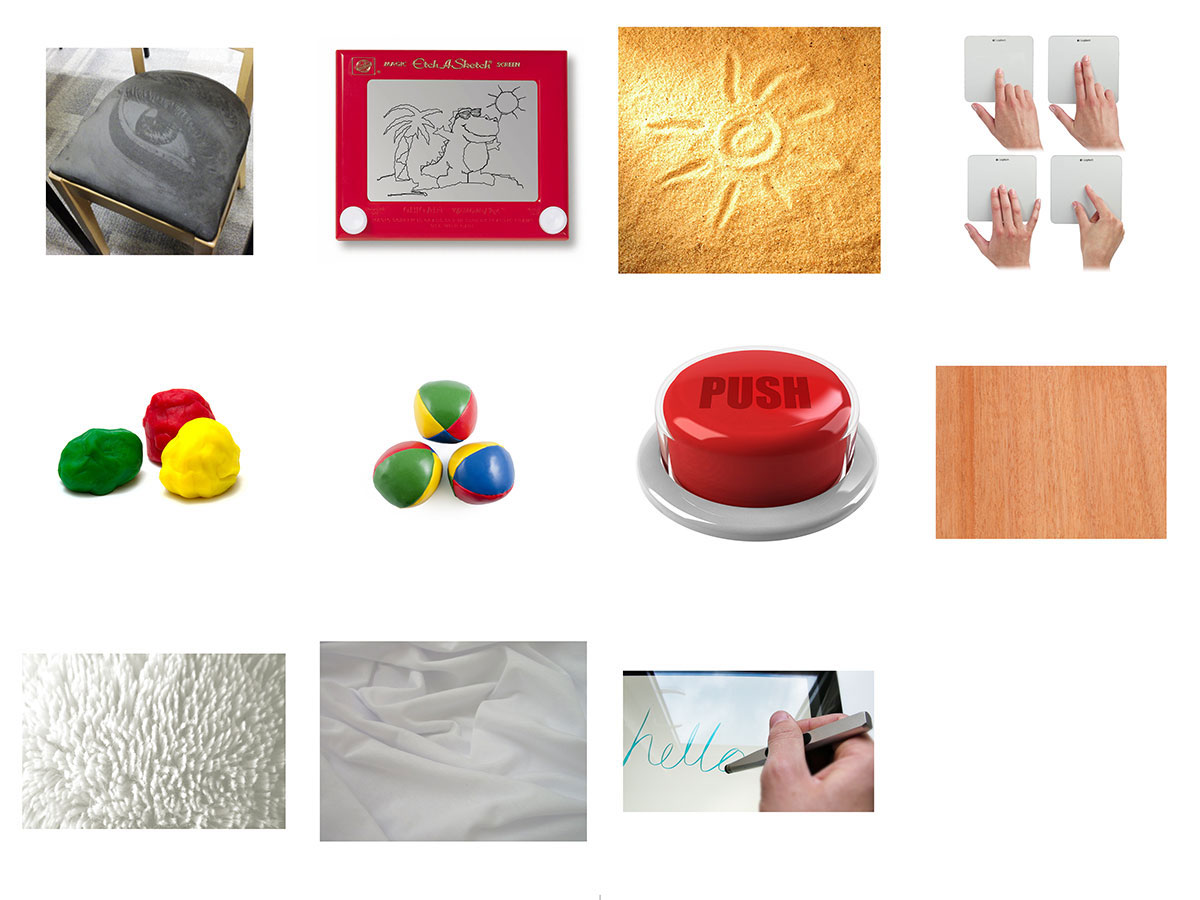
\includegraphics[width=0.9\linewidth]{workshops/technology-cards}
  \captionof{figure}{Technology cards}
  \label{ch:workshops:technology-cards}
\end{minipage}%
\begin{minipage}[t]{.5\textwidth}
  \centering
  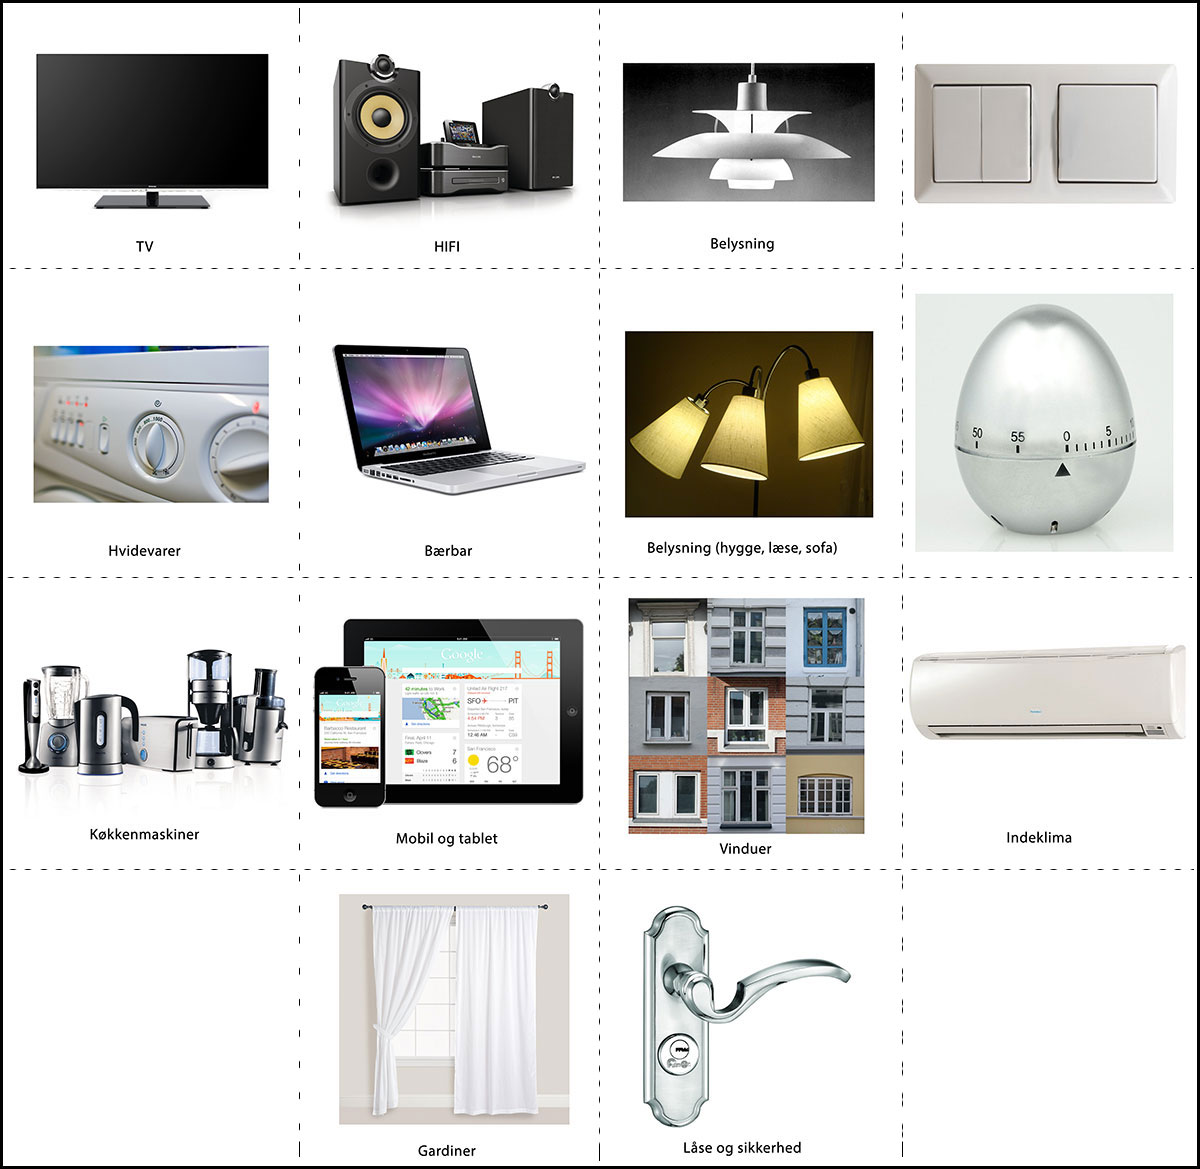
\includegraphics[width=0.9\linewidth]{workshops/appliance-cards}
  \captionof{figure}{Appliance cards}
  \label{ch:workshops:appliance-cards}
\end{minipage}
\end{figure}

\subsection{Discussion}


\section{Discussion}

\todo{Conventions and the familiarity of the home ... Dindler, 2010 - Lerdahl, Bell, Ehn...} Were we successful in defamiliarising the home setting???



\chapter{Prototyping: Let's Jam}
\label{ch:jamming}
%!TEX root = thesis.tex

\todo{Maybe some Gaver (research through design) and (Alternatives, conceptual design proposals )}

A lot of things jam; cars do it in traffic, musicians do it during a rehearsal, paper does in printers, and we might even put it on bread.
In this chapter particles jam.
\blank
As mentioned in our definition of AHIs in \autoref{ch:adhoc} we proposed three different approaches to creating AHIs.
In this chapter we will explore the first approach which was to use shape-change as a construction mechanism for AHIs.
So in this chapter we will dig in to the area of shape-changing interfaces to explore and illustrate the possibilities of creating AHIs based on shape-change.
More specifically we will touch upon a specific approach to constructing SCIs called jamming.

SCIs were introduced in the introduction of this thesis as interfaces that use physical change of shape as input or output.
Jamming is a special kind of technique that can be used to control the stiffness of a material which makes it possible to construct objects that can change their surface structure.

What makes SCIs interesting to AHIs is their ability to dynamically change the physical properties of an interface element, be it shape, texture, stiffness, position ect.
This change in physicality can then be the offset for a new temporary interaction possibility that is created for the specific situation, where afterwards it can return to it's initial natural state.
Compared to TUIs, SCIs have the ability to form a dynamic relationship between the physical objects and the digital state of the system, allowing both the user and the computer to change the physical state of an object to match its digital state.
These aspect align well with the definition of AHIs that we presented earlier in section~\ref{adhoc:definition}.
\blank
The process of our exploration of SCIs has, at times, been somewhat discouraging as we have proceeded to learn the lessons of the difficulty of creating such interfaces.
We have come to the conclusion that SCIs are indeed non-trivial to build and prototype, a lesson that we think everyone who has worked on SCIs must have experienced at some point, although it has not been widely mentioned in the literature. 

There are some inherently difficult aspects of creating objects with kinetic movements, for example in our earlier described BeoMotion project the change from flat surface to edged surface proved difficult as the phase change, because we worked with non-elastic materials, caused a contraction of the base structure.
We solved this by putting small rails on each of the individual elements of the structure to allow the contraction but this caused a new problem as small gaps now emerged since the base of the elements was able to move sightly in relation to each other.

In our exploration of jamming we also ran in to various problems.
While we consider ourselves fairly home in physical computing we, perhaps a little overconfident, initially thought it would be moderately straight forward to build pneumatic and hydraulic jamming systems.
We quickly ran into difficulties though with a seemingly continuous stream of new challenges in relation to vacuum pumps, compressors, solenoid valves, custom made membranes, various fittings and connectors between non-fitting tubes, particles and filters -- all elements that we had never worked with before, see figure \ref{fig:ch:jamming:materials}.
On top of that all of these pieces had to work together while being air or water tight. 

So while we did not end up with a finished, ready-to-test prototype we did still, in our opinion, gain relevant experiences and additions to our notion of AHIs, in the shape of concrete experience with building AHIs, concept development and a study of the field of jamming and its relevance to AHIs. 

\begin{figure}[h]
	\centering
	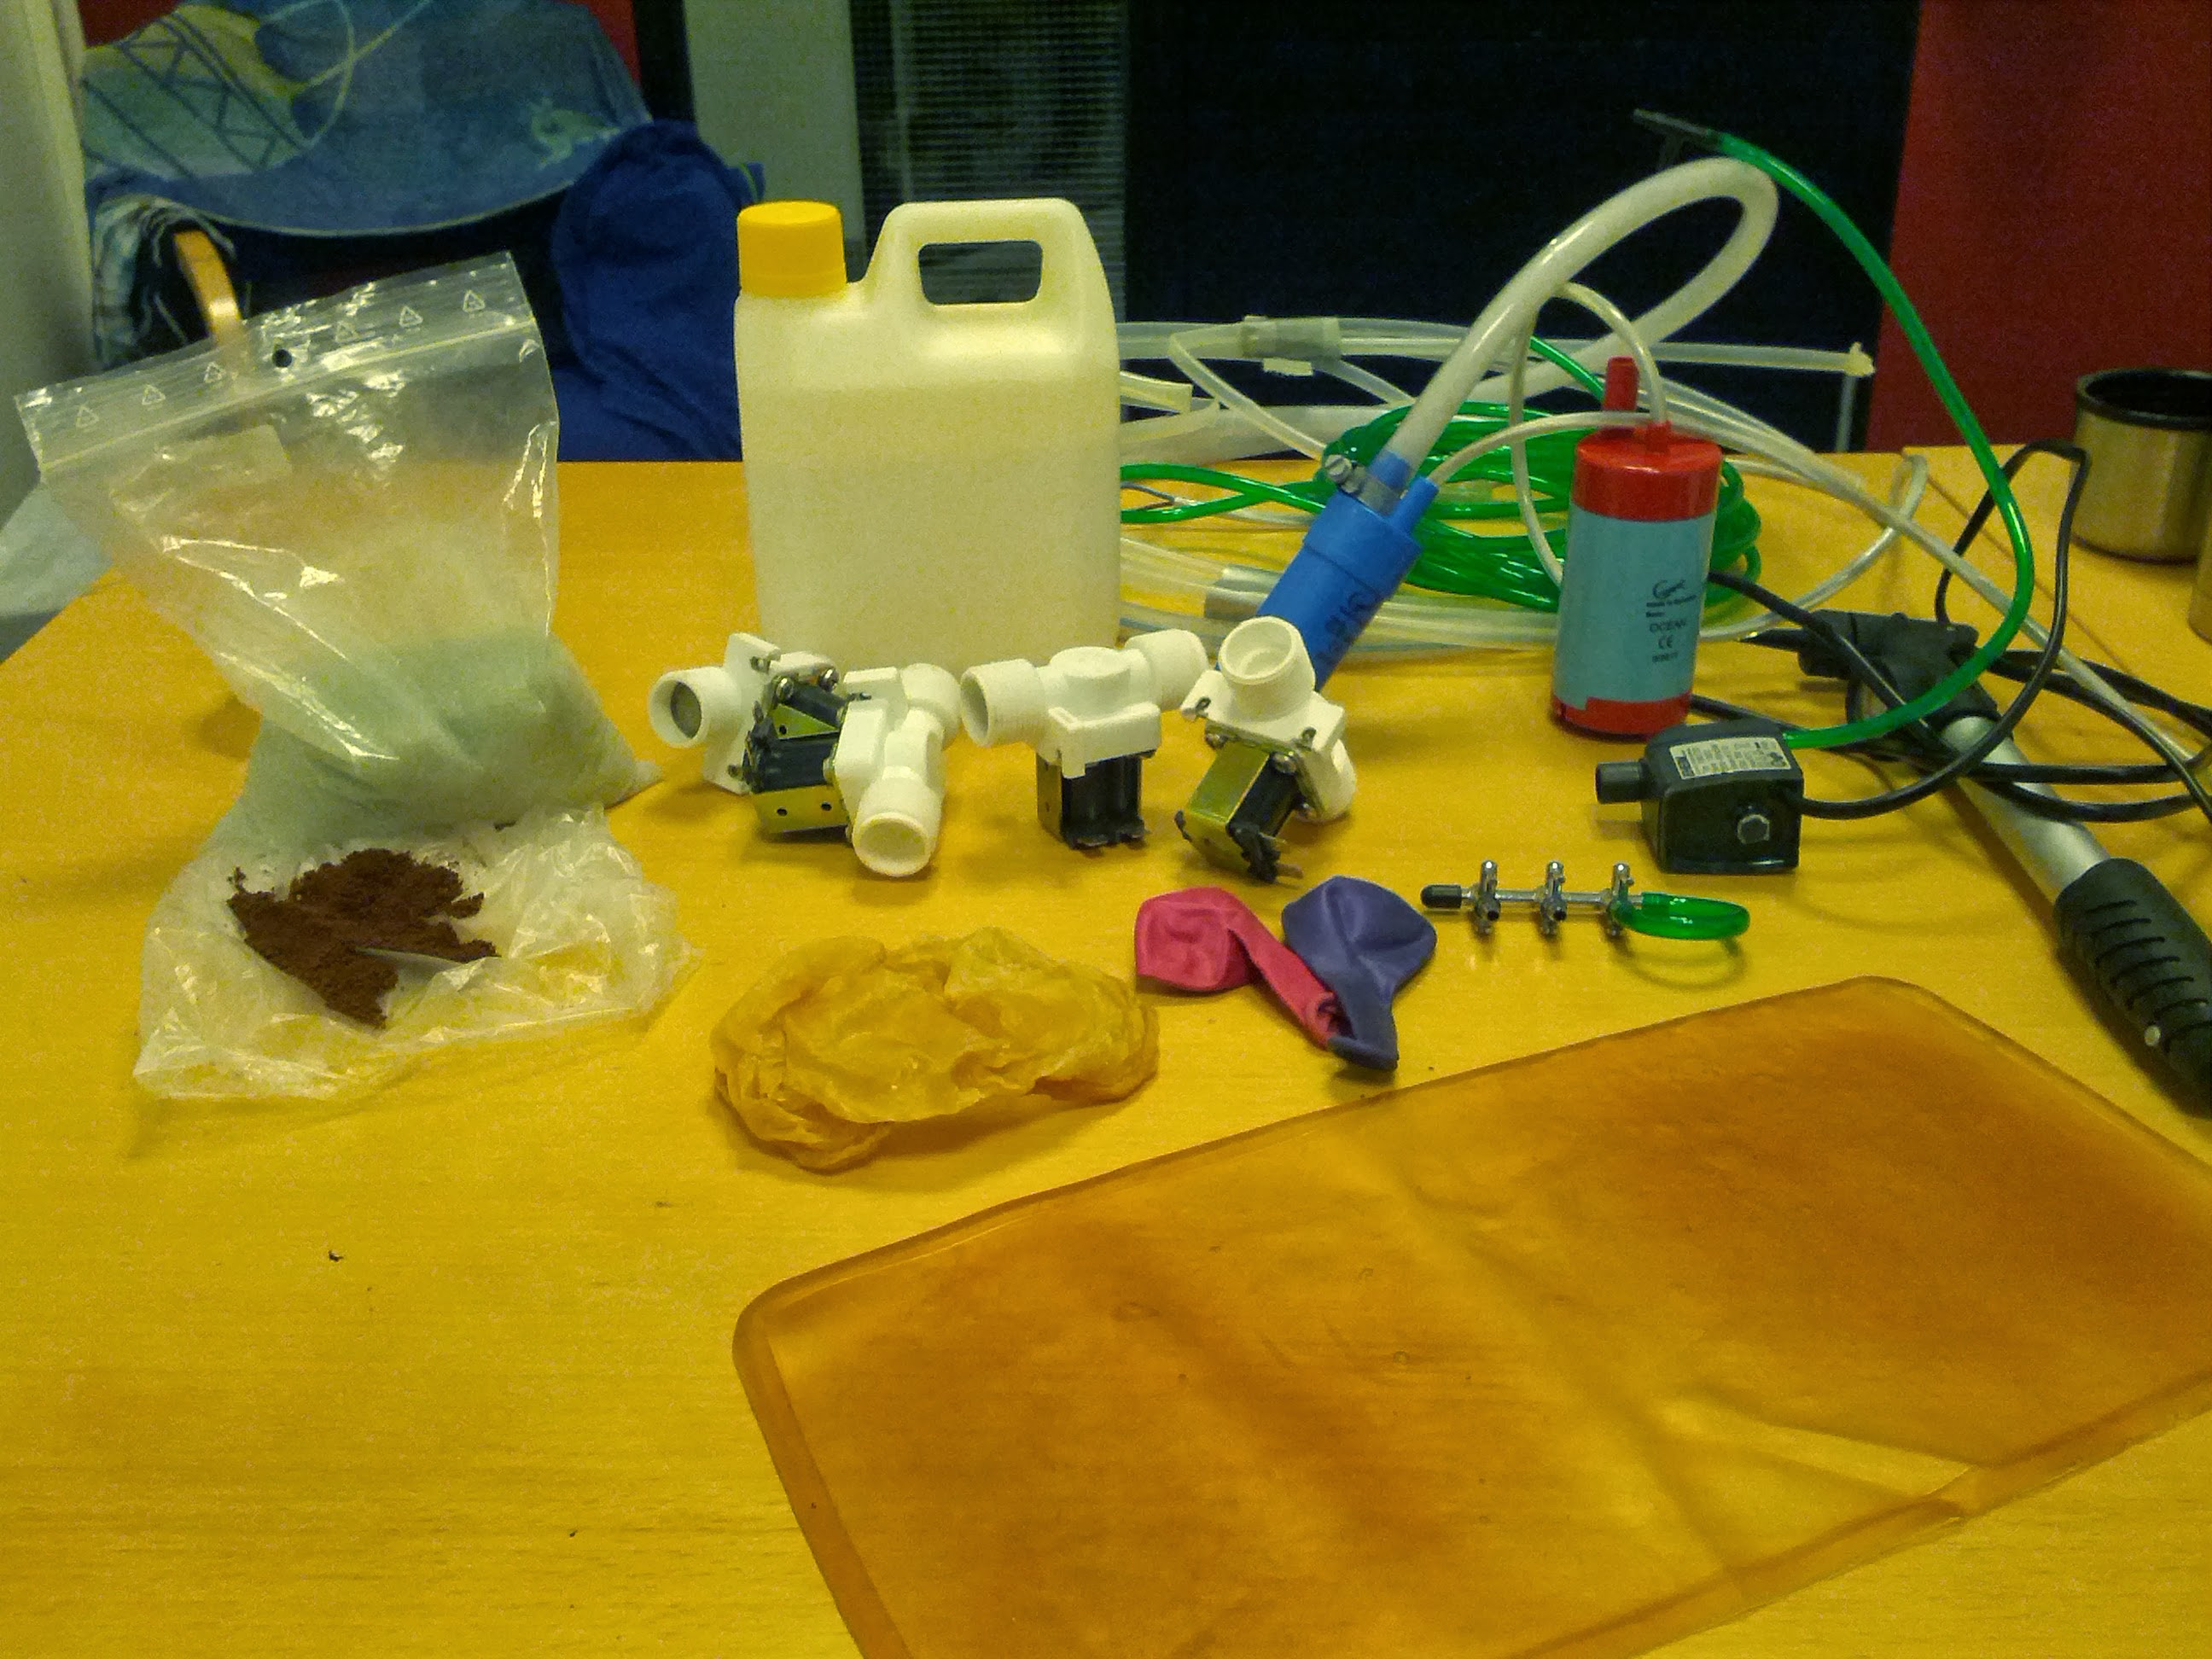
\includegraphics[width=.9\linewidth]{figures/jamming/jamming-materials}
	\caption{A selection of the materials we acquired and used for a jamming system. \textbf{Far left:} glass-beads and ground coffee which were used as granular material. \textbf{Front:} custom membranes made from rubber milk (white container in background) and balloons. \textbf{Center:} white solenoid valves for electronic control of the flow of fluid and a manual valve next to the balloons. \textbf{Right:} three different electronic pumps for moving fluids and lastly a manual pump.}
	\label{fig:ch:jamming:materials}
\end{figure}

\section{A vocabulary of shape-change}
\label{ch:jamming:shape-change} 
%!TEX root = ../thesis.tex
\todo{more introduction, back-reference to chapter 3}

\todo{SCI chapter needs review to make it more relevant to the prototyping}

Shape-changing interfaces (SCIs) are a relative new subject in the area of human-computer interaction.
In previous work it has been discussed under various different terms such as Kinetic Interaction, Organic User Interfaces, Actuated Interfaces, to name a few stated by \citet{rasmussen2012shape}.

\subsection{A vocabulary of shape-change}
\label{ch:jamming:vocabulary}
In this chapter we will expand our vocabulary regarding SCIs based on \citet{coelho2011shape} and \citet{rasmussen2012shape}.
They both provide contributions as to how we can talk about SCIs, how we can group and identify different types of change of shape, how we can identify and describe shape transformations, and most importantly, how and to which purpose we can interact with SCIs.
We will use this vocabulary onwards in our thesis to discuss SCIs, both ours and others.   
Rasmussen defines shape-changing interfaces as
\begin{quotation}
  \emph{A shape-changing interface uses physical change of shape as input or output.}
\end{quotation}
and further
\begin{quotation}
  \emph{[\ldots] the self-actuation must be controllable so that the object can return to its initial state and repeat the shape change. }  
\end{quotation}

\citeauthor{coelho2011shape} presents a grouping which distinguish three types of change of shape: \emph{topological, textural and permeable} transformations.
Topological transformations here being those transformations which adhere to topological equivalence, permeable those which do not and textural transformation stands as a category for it. Topologically equivalence here means that a form can transform in to another form by a continuously homeomorphic transformation - that is without cutting or gluing either form. This can be exemplified by the pliable donut that transforms into a coffee mug without breaking homeomorphism as seen in figure~\ref{pliable-mug} \todo{lav egen figur?} 

\begin{figure}[hb]
	\centering
  		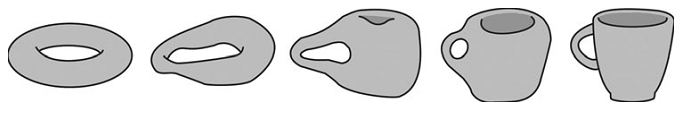
\includegraphics[width=4in]{figures/pliable-donut}
	\caption[The pliable donut momeomorphic transformation, taken from \citep{coelho2011shape}]
   {The pliable donut momeomorphic transformation, taken from \citep{coelho2011shape}}
   \label{pliable-mug}
\end{figure}   
 
\citeauthor{rasmussen2012shape} suggests a grouping more detailed grouping of shape-changing interfaces by identifying eight types of change of shape, namely: \textit{orientation, form, volume, texture, viscosity, spatiality, adding/subtracting and permeability}.
These eight fit into two groups where the first six are topologically equivalent and the last two are not. This is in line with what \citeauthor{coelho2011shape}, though texture standing has been moved into the topologically equivalent group. Overall it expands on \citeauthor{coelho2011shape}s work and enables us to identify and discuss form changes in more detailed terms.
The grouping is visualized in figure~\ref{types-of-change}, illustrating the different types of change.

\begin{figure}[hb]
	\centering
  		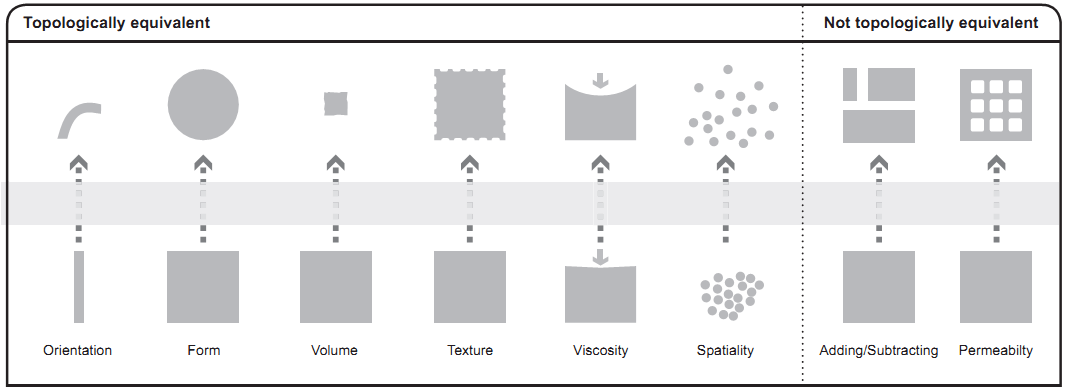
\includegraphics[width=4in]{figures/types-of-change}
	\caption[Types of shape-change as visualised by \citep{rasmussen2012shape}]
   {Types of shape-change as visualised by \citep{rasmussen2012shape}}
   \label{types-of-change}
\end{figure}

There might be some debatable cases in this grouping, e.g. they define textural change as
\begin{quotation}
small changes on the surface of the shape that add visual and tactile properties without affecting the overall form
\end{quotation} 
so if the overall form is not changed it might not make sense to classify it as a homomorphic transformation, which might also be the reason why \citeauthor{coelho2011shape} chose to separate it as a case for itself.
Also if we look at the case of spatiality changes where a collection of elements form a single object, it is possible to think of examples where non-homeomorphic transformations occurs if, for example, the collection of elements split in the middle forming two objects and then merge back together.
This would still count as a shape-changing interface as described in the definition but would not adhere to topological equivalence.   

The transformation in itself is interesting as well and \citeauthor{rasmussen2012shape} reveals different types of transformation.  They describe the transformation as the \textit{phase between endpoints}, meaning the phase between the form's origin and its morphed state.
They distinguish between kinetic parameters and expressive parameters, where
the kinetic parameters describe the physical movements of the transformation and the expressive parameters relates to how the kinetic movements are perceived and understood.
This is a very interesting and important aspect of SCIs since it, together with the theory of affordances, provides the basis for understanding the interface and its functions, which at the same time is one of the key challenges of SCIs.
Since SCIs are inherently non-static objects we might not be able to rely on the form alone to communicate the intent and functions of the object, so there might have to be some interaction clues elsewhere, for example in the transformation itself. This will be discussed in more detail in chapter \todo{ref somewhere}  

A key aspect of SCIs, and any user interface in general, is the interaction - be it direct physical interaction, implicit visual interaction, or something in between. 
\citeauthor{rasmussen2012shape} distinguish between \textit{no interaction}, where there is only shape-changing output; \textit{indirect interaction}, still only with shape-changing output but based on implicit user input; \textit{direct interaction}, where the user deforms the object in some way as user input and a shape-change output occurs, either in the object itself or in a remote object.
Two approaches to direct interaction are identified, \textit{action and reaction} where the object reacts directly to the action in a synchronized process and \textit{input and output} where the object is acting asynchronously and not necessarily directly related to the input.    
Our focus will be on objects with direct interaction and mainly those with input and output merged into the same object, as we here see the best possibilities for creating interfaces \todo{et eller andet}
 
\hl{Our own exploratory work will focus only on topological transformations, excluding spatiality, since our choice of technology hinders this type of change.} This will be further described in section \todo{ref til proto 0}  

\section{Jamming as an enabling technology}
\label{ch:jamming:enabling-technology} 
%!TEX root = ../thesis.tex
Before continuing on the topic of jamming, let's first give an introduction to the mechanics of jamming.

Jamming is a mechanism that can enable granular material to transition between solid-like and liquid-like states. These states can occur if the material is put under an external stress, figure~\ref{fig:ch:jamming:phase-transition} illustrate these states.
Much like water can shift to gas when heated and to ice when cooled. But where water is affected by thermodynamics, granular systems are not. \hl{entirely true?}
Sand, which is a granular material, may resemble a liquid as it flows through an hour glass, although the individual grains themselves are a solid structure. This is due to something called \todo{Jamming, Force chains and Fragile matter}

\begin{figure}[hb]
	\centering
  		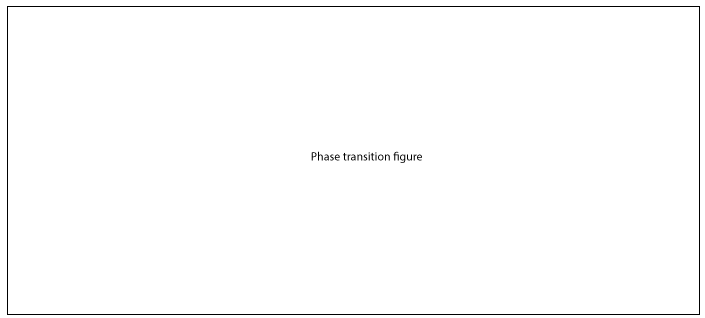
\includegraphics[width=4in]{figures/jamming/phase_transition}
	\caption[Phase transition from \textit{liquid} state to \textit{solid} state.]
   {Phase transition from \textit{liquid} state to \textit{solid} state.}
   \label{fig:ch:jamming:phase-transition}
\end{figure}

You might have noticed how some coffee packagings at the local super market are like a rigid container, see figure~\ref{fig:ch:jamming:coffee-packaging}. 
In this kind of packaging, after filling it with coffee, all excess air has been sucked out by applying a vacuum, i.e. jamming the coffee grains, and thereby making it almost rock solid. 
Also, think about a regular bean bag which exhibits some of the same properties, see figure~\ref{fig:ch:jamming:bean-bag}. 
When no force is applied to it, i.e. no one is sitting in it, it resembles the liquid-like state mentioned earlier. 
When a person then sits down in a bag air will be pressed out and the particles (most often polystyrene foam) will be pushed tightly together filling the voids  \todo{some physical term here, phase space and stuff} thereby jamming the particles making it resemble a solid ...

\begin{figure}
\centering
\begin{minipage}[t]{.5\textwidth}
  \centering
  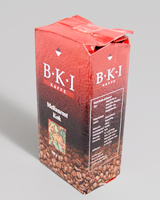
\includegraphics[width=.4\linewidth]{figures/jamming/coffee_packaging}
  \captionof{figure}{Coffee in vacuum packaging}
  \label{fig:ch:jamming:coffee-packaging}
\end{minipage}%
\begin{minipage}[t]{.5\textwidth}
  \centering
  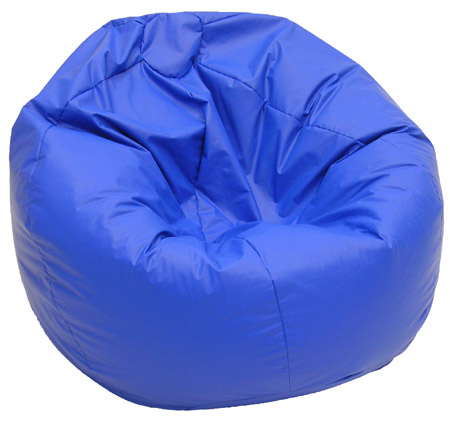
\includegraphics[width=.4\linewidth]{figures/jamming/bean_bag}
  \captionof{figure}{A bean bag}
  \label{fig:ch:jamming:bean-bag}
\end{minipage}
\end{figure}

\subsection{Particles}
\label{ch:jamming:particles}
The granular material, also called the particles, can be any material that has the physical properties that allow for jamming to occur. 
But parameters such as particle size, shape and compressibility have an impact on the jamming transition. 
This has been investigated by several researchers, e.g. \cite{cheng2012design} and \cite{steltz2010jamming}, where the stress to strain ratio \todo{explain this} of different granular materials are evaluated. 
Ground coffee (fine and coarse) and glass beads of varying size are recurring across these tests, the first being an irregular shape with a rough surface as opposed to the plain shape and smooth surface of the second, see figure~\ref{fig:ch:jamming:particles-close-up}. 
Particles of same size and with a smooth surface will tend to be more fluid-like when unjammed as they flow more freely. 
Irregular particles with rough surfaces will create more friction between the particles thus being less fluid-like in the unjammed state.

The conclusion is that the choice of granular material is very much dependent on the application in question. 

\begin{figure}
\centering
\begin{subfigure}{.5\textwidth}
  \centering
  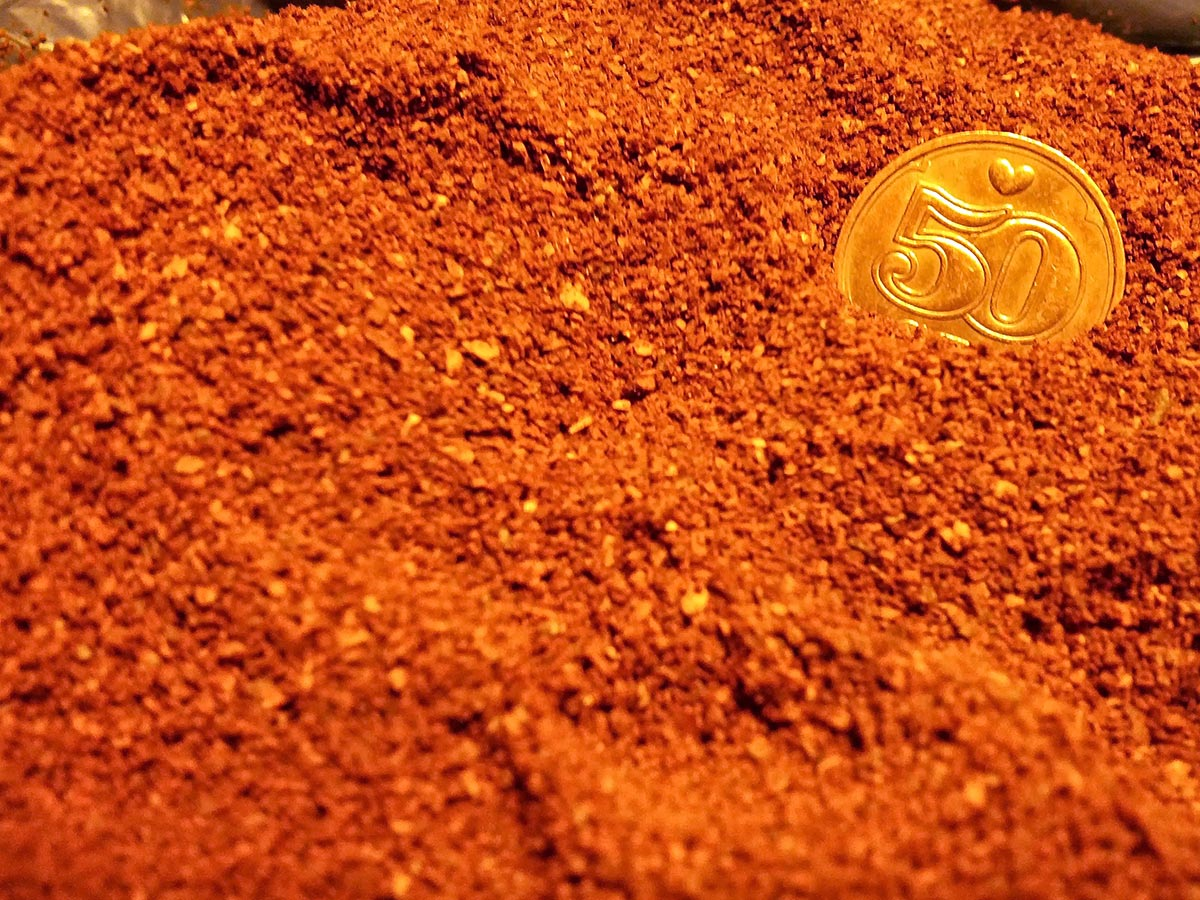
\includegraphics[width=.9\linewidth]{figures/jamming/coffee-grains}
  \caption{Grounded coffee}
  \label{fig:sub1}
\end{subfigure}%
\begin{subfigure}{.5\textwidth}
  \centering
  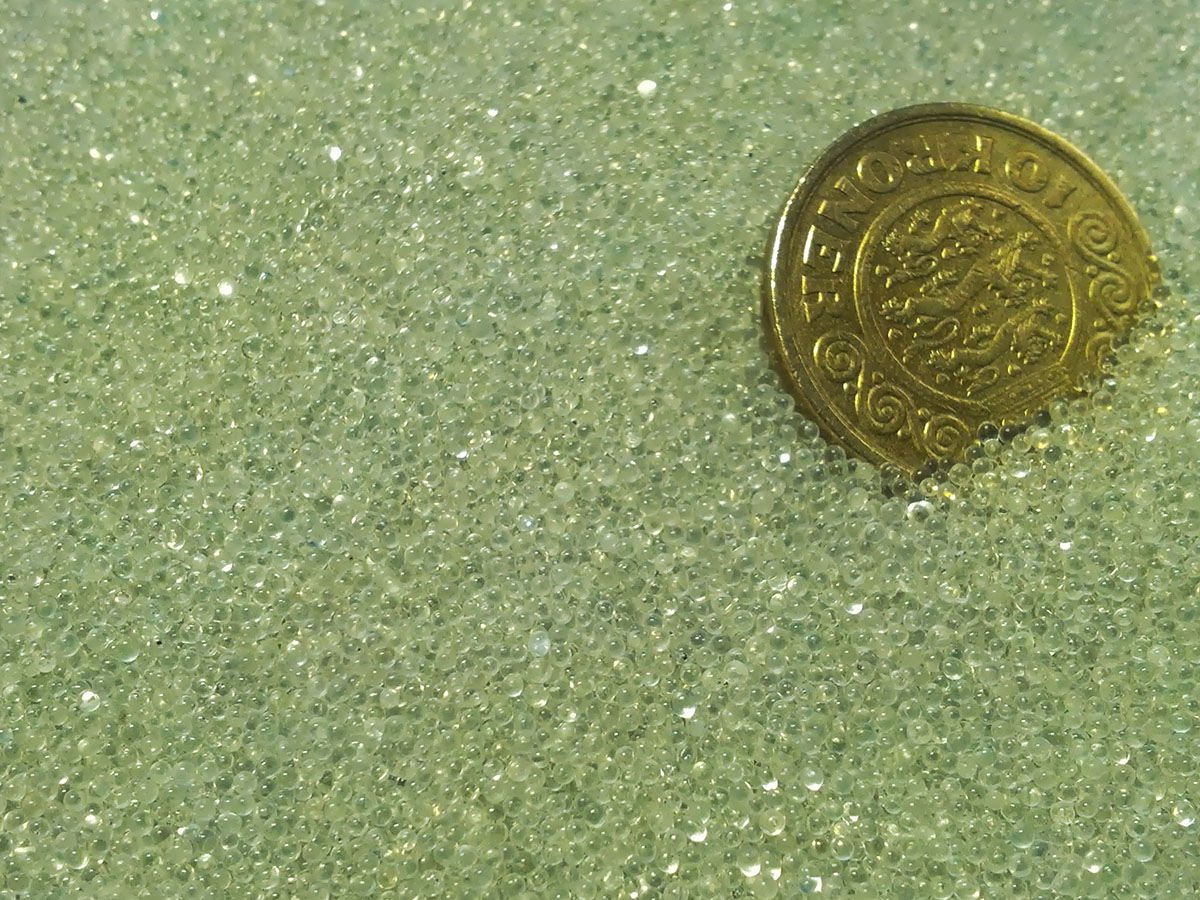
\includegraphics[width=.9\linewidth]{figures/jamming/glass-beads}
  \caption{Glass beads}
  \label{fig:sub2}
\end{subfigure}
\caption{A microscopic view of different granular material.}
\label{fig:ch:jamming:particles-close-up}
\end{figure}

\todo{research in particle parameters in other\\ disciplines such as robotics.}

\begin{itemize}
	\item http://en.wikipedia.org/wiki/Jamming\_(physics)
	\item http://www.nature.com/nphys/journal/v3/n4/full/nphys580.html
	\item http://www.nature.com/nature/journal/v411/n6839/full/411772a0.html
\end{itemize}

\subsection{The technique}
\label{ch:jamming:technique}

The jamming technique can be applied with both a pneumatic and a hydraulic approach.
In the pneumatic approach a gas, for example air, is used as a means for actuation, see figure~\ref{fig:ch:jamming:jamming-basics}.
The gas is enclosed together with granular material within a flexible and air tight container, for example rubber latex. 
A filter prevents the granular material from escaping the container and a valve upholds the pressure.
An external vacuum pump can then suck out the air of the container, creating a negative pressure inside, which results in the transition to a solid-like form. 
The speed of this transition of course depends on the suction power of the pump.
When the vacuum is released the form will gradually transition back to the liquid state. 
In this way, the transition allows for states in between the two extremes; solid and liquid.

Jamming makes it possible to deform an object by hand while in the liquid state and then apply the vacuum and make the deformed object solid - in a sense the form is \emph{saved} as long as the vacuum is maintained.
Figure~\ref{fig:ch:jamming:jamming-transition} shows a transition where a form has been molded and solified into a shape.
When the pressure is released the form gradually changes shape as seen in the individual steps of the figure.
In the setup a balloon was used as the membrane and ground coffee within as particles.
Pressure was applied with a vacuum cleaner and a coffee filter prevents the particles from being sucked out.

In the example it can be seen that the object (balloon) returns to its initial state which is a requirement for SCIs as stated earlier in section \ref{ch:jamming:vocabulary}.
In this example it is the tension of the latex of the balloon that forces it back but it could as well have been an actuation done with the jamming technique itself. 

\begin{figure}[hb]
	\centering
  		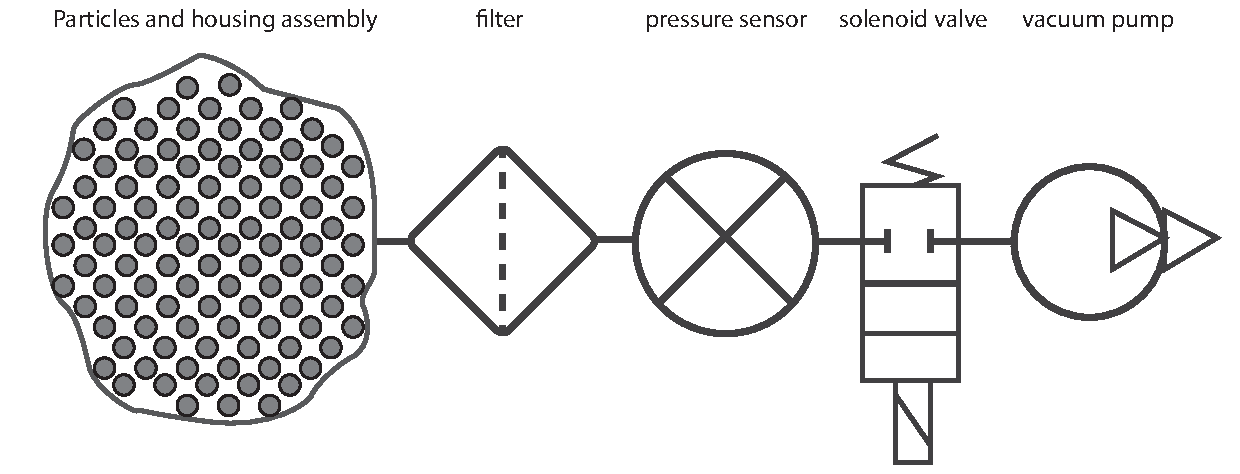
\includegraphics[width=4in]{figures/jamming/jamming-basics}
	\caption[A basic pneumatic jamming system.]
   {A basic pneumatic jamming system.}
   \label{fig:ch:jamming:jamming-basics}
\end{figure}

\begin{figure}[hb]
  \centering
      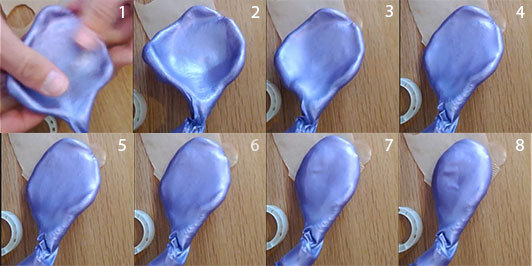
\includegraphics[width=\textwidth]{figures/jamming/jamming-transition}
  \caption[A jamming transition setup.]
   {Jamming transition with a balloon, grounded coffee, vacuum cleaner and a coffee filter.}
   \label{fig:ch:jamming:jamming-transition}
\end{figure}



\section{Related work}
\label{ch:jamming:related-work} 
%!TEX root = ../thesis.tex
Although jamming might seem as a novel approach in the area of HCI, other areas of research have had it on their agenda for some time. 
Especially in the area of mechanical engineering where the jamming mechanism has shown promising results in robotic applications as a substitute for mechanical parts.
In the following we cover the current applications of jamming in both HCI and engineering. 

\subsubsection{Mechanical engineering and robotics}

\citet{brown2010universal} and \citet{amend2012positive} used the jamming technique to develop a universal robotic gripper, which is the tool at the end of a robotic arm that interacts with its environment.
This is an example of the basic jamming approach with a single volume, as in figure~\ref{fig:ch:jamming:approaches:basic}.
The gripper was simply built with an elastic bag as a container for the granular material, which was chosen to be grounded coffee. 
It is able to pick up objects of heterogeneous shapes due to the gripper simply adapting to the surface structure of the objects on impact, see figure~\ref{fig:ch:jamming:jamming-robot-gripper}. 
Contrasting this with a normal mechanical robotic arm which needs several actuators to grap objects of heterogeneous shapes, this gripper is implemented with a single actuator, the jamming volume, which still obtains multiple degrees of freedom (DoF).

\begin{figure}[h]
  \centering
  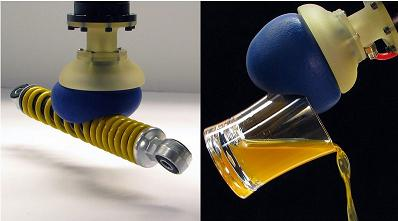
\includegraphics[width=0.9\linewidth]{figures/jamming/jamming-robot-gripper}
	\caption[A universal robotic gripper based on the jamming of granular material by \citet{brown2010universal}.]
   {A universal robotic gripper based on the jamming of granular material \citep{brown2010universal}.}
   \label{fig:ch:jamming:jamming-robot-gripper}
\end{figure}

Jamming is also seen in experiments with autonomous robots where the mechanism can be used as artificial muscles.
\citet{steltz2009jsel} used the jamming technique to create a platform for shape-changing and mobile robots called JSEL (Jamming Skin Enabled Locomotion).
As opposed to the previous example this work is based on the cell-based jamming approach, as seen in \ref{fig:ch:jamming:approaches:cell}.
The soft robot can morph its ``skin'' to create movement of the entire body by controlling the stiffness of the individual cells and inner actuator (see figure~\ref{fig:ch:jamming:jsel}). 

\citet{steltz2010jamming} took the JSEL approach further combining the cell-based approach with a linear actuator. 
The assembly combines the contraction and extension capabilities of the linear actuator and modulates this 1-DoF actuation into a multi-DoF actuator depending on the number of surrounding jamming cells.
The platform is called JMU (Jamming Modulated Unimorph) and has been tested as component segments of a worm, as an example of a soft robot (see figure~\ref{fig:ch:jamming:jmu}).

These different examples from other fields of research illustrate how creative implementations of the jamming technique can substitute mechanical parts and in many ways simplify the implementation.

\begin{figure}
  \centering
  \begin{minipage}[t]{.44\textwidth}
    \centering
    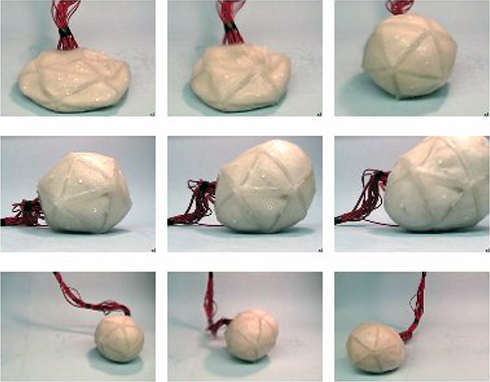
\includegraphics[width=\linewidth]{figures/jamming/chembot-robot-blob}
    \caption[Jamming Skin Enabled Locomotion (JSEL) by \citet{steltz2009jsel}.]
    {Jamming Skin Enabled Locomotion (JSEL). Each cell can be jammed individually to create motion \citep{steltz2009jsel}.}
    \label{fig:ch:jamming:jsel}
    \hspace{.2\textwidth} 
  \end{minipage}%
  \hspace{0.02\textwidth}
  \begin{minipage}[t]{.44\textwidth}
    \centering
    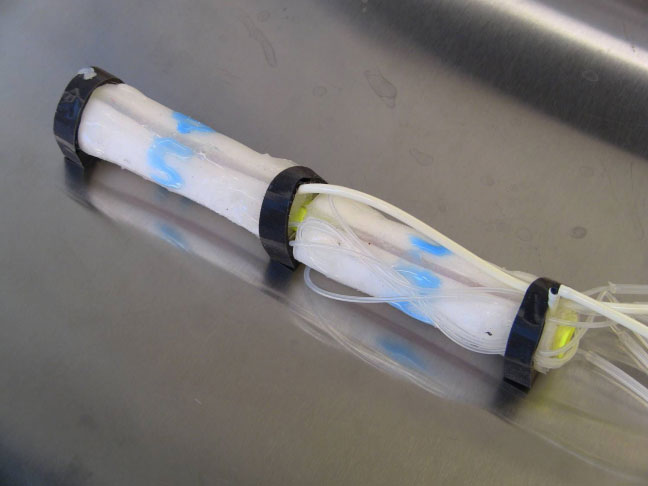
\includegraphics[width=\linewidth]{figures/jamming/jmu-worm}
    \caption[Jamming Modulated Unimorph by \citet{steltz2010jamming}.]
    {Jamming Modulated Unimorph \citep{steltz2010jamming}.}
    \label{fig:ch:jamming:jmu}
  \end{minipage}
\end{figure}

\subsubsection{Human-computer Interaction}
\label{ch:jamming:related-work:hci}
Jamming has also been explored in the area of HCI though to a limited extent.
Most of the examples here are very recent contributions (2012) but they do show promising applications.

\paragraph{Dynamically changeable physically buttons (\citeyear{harrison2009providing})} 
\label{ch:jamming:related-work:hci:dynbuttons}
This first example is actually not based on jamming but on some of the same principles, where pneumatic actuation is used to enable deformations on a latex surface.
The project presents a visual display which contains deformable areas able to create physical buttons.
An acrylic backing layer with cut-out areas for the shapes and positions of the buttons are placed under an upper latex surface.
With pneumatic control it is possible to dynamically make physical buttons appear at the cut-out areas as either convex, concave, or flat forms, see figure~\ref{fig:ch:jamming:concepts:harrisonhudson}.
Though button states can be modified they are still in a very static configuration due to the cut-out areas which cannot be changed.

\begin{figure}[h]
  \centering
  \begin{minipage}[b]{.8\textwidth}
    \centering
    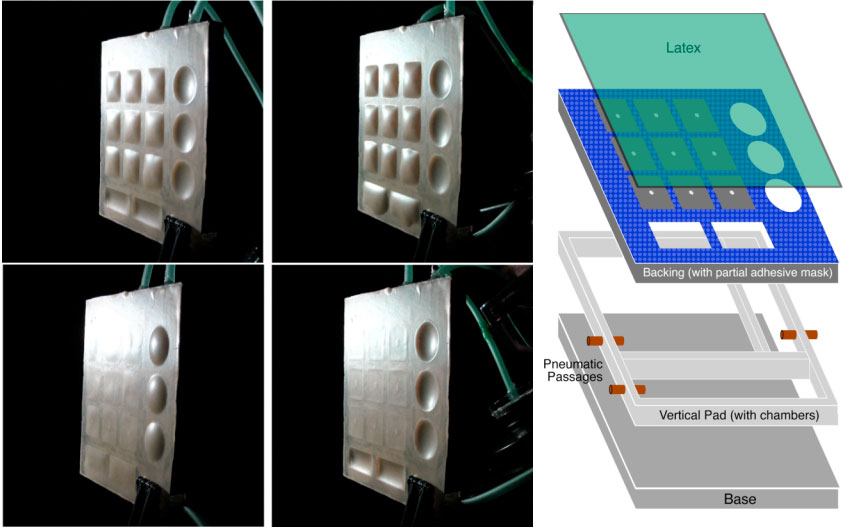
\includegraphics[width=.7\linewidth]{figures/jamming/harrisonhudson}
    \caption{A tactile display in various interface states. All buttons are statically positioned \citep{harrison2009providing}.}
    \label{fig:ch:jamming:concepts:harrisonhudson}
  \end{minipage}
\end{figure}

\paragraph{The HoverMesh (\citeyear{mazzone2004hovermesh})}
\label{ch:jamming:related-work:hci:hovermesh}
\citet{mazzone2004hovermesh} did some early work on creating a deformable structure with the jamming technique. 
The HoverMesh prototype is a cell-based jamming system consisting of 3x3 grid, see figure~\ref{fig:ch:jamming:hovermesh}.
The grid is mounted on top of a cubicle which can be inflated and deflated and together with the grid it creates deformations of the surface structure.
The HoverMesh prototype is not fully implemented according to the ideas presented.
It consists only of the grid structure on top of the cubicle and does not exhibit input capabilities through vision-based techniques and haptic feedback output as intended. 

\paragraph{ClaytricSurface (\citeyear{matoba2012claytricsurface})}
\label{ch:jamming:related-work:hci:claytric}
\citet{matoba2012claytricsurface} created a flexible tabletop surface, ClaytricSurface, which serves as a sculptable display medium (see figure~\ref{fig:ch:jamming:claytric-surface}). 
The surface can be directly manipulated by hand and the stiffness can be controlled in real time by a GUI slider.
Input is detected by a depth camera from above the tabletop.
The exemplified application of ClaytricSurface is a painting application projected onto the surface from above and a user can use direct touch on the surface to draw. 
ClaytricSurface uses the basic jamming approach and demonstrates the use of a rather large jammable surface area with direct manipulation abilities.

\begin{figure}
  \centering
  \begin{minipage}[t]{.44\textwidth}
    \centering
    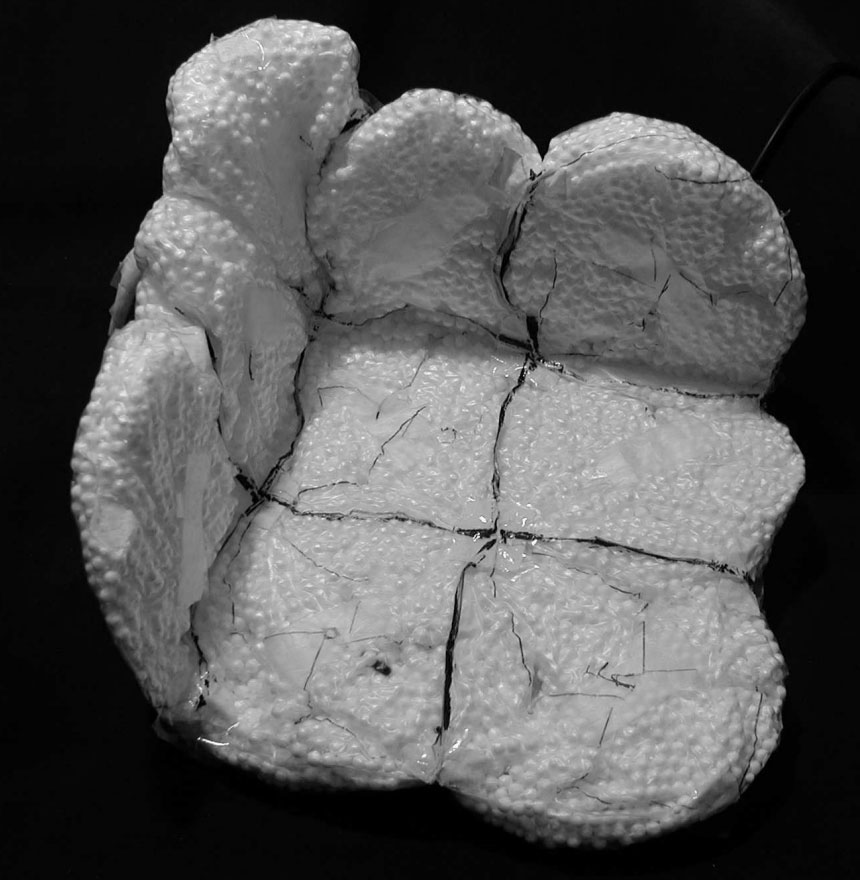
\includegraphics[width=\linewidth]{figures/jamming/hovermesh}
    \caption[The HoverMesh by \citet{mazzone2004hovermesh}.]
    {The HoverMesh \citep{mazzone2004hovermesh}.}
    \label{fig:ch:jamming:hovermesh}
  \end{minipage}%
  \hspace{0.02\textwidth}
  \begin{minipage}[t]{.44\textwidth}
    \centering
    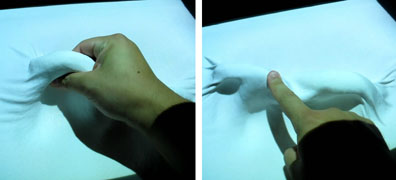
\includegraphics[width=\linewidth]{figures/jamming/claytric-surface}
    \caption[Claytric Surface by \citet{matoba2012claytricsurface}.]
    {Claytric Surface \citep{matoba2012claytricsurface}.}
    \label{fig:ch:jamming:claytric-surface}
  \end{minipage}
\end{figure}

\paragraph{Jamming User Interfaces (\citeyear{follmer2012jamming})}
\label{ch:jamming:related-work:hci:jui} 
\citet{follmer2012jamming} have probably made the biggest contribution yet to the use of jamming in HCI. 
The authors coin the approach \textit{Jamming User Interfaces} and position it in the area of malleable and organic user interfaces. 
They make several contributions to the field by exploring jamming interfaces for haptic feedback, for malleable tabletops and for mobile devices (see figure~\ref{fig:ch:jamming:jui-collection}). 
They also investigate how sensing techniques like capacitive and optical sensing, can broaden the applicability of jamming in HCI. 

\citet{follmer2012jamming} also present a hydraulic jamming system that is fast and silent and which allows for semi-transparent jamming volumes. 
This requires transparent particles, such as glass-beads, and a transparent fluid that matches the refractive index of the particles so that light refraction is reduced, see figure~\ref{fig:ch:jamming:jui:refractive}. 

\begin{figure}[h]
  \centering
  \begin{minipage}[b]{.7\textwidth}
    \centering
    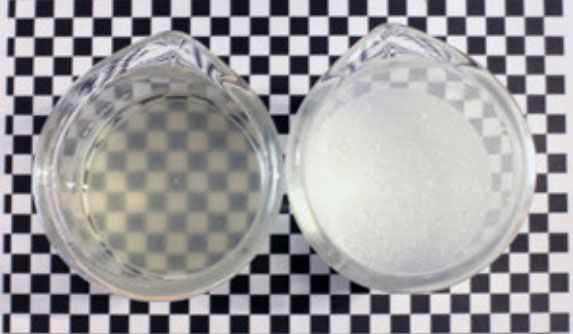
\includegraphics[width=.5\linewidth]{figures/jamming/refractive-index}
     \caption{Transparency obtained by matching the refractive index of the glass-bead particles \citep{follmer2012jamming}}.
    \label{fig:ch:jamming:jui:refractive}
  \end{minipage}
\end{figure}

In the following we will give a brief overview of the four prototypes implemented and described by \citet{follmer2012jamming}.

\subparagraph{Tunable Clay} is a malleable tabletop for direct 3D modelling (see figure~\ref{fig:ch:jamming:jui-clay}).
It resembles ClaytricSurface \citep{matoba2012claytricsurface} mentioned earlier with its clay-like surface that can easily be deformed (basic jamming approach).
Tunable Clay uses the hydraulic jamming system mentioned above with index-matched particles and fluid.
This allows for a more sophisticated depth sensing approach than the one used with ClaytricSurface.
Optical shape sensing and graphic projection is integrated underneath the jamming volume.
The shape, captured in real-time, is shown as a virtual 3D model on both an external display and on the jamming volume itself projected from underneath the surface.

\subparagraph{Transparent Haptic Lens} is a small tangible puck to be used as a haptic information channel on a tabletop display (basic jamming approach), see figure~\ref{fig:ch:jamming:jui-lens}.
It has a transparent lens in the center which is a transparent hydraulic jamming volume that can change its stiffness according to the texture beneath it.
By pressing ones finger into the lens the user can get a haptic sensation through stiffness reflecting the underlying texture of the image directly underneath. 

\subparagraph{Behind-the-Tablet Jamming} is a tablet computer which has a pneumatic jamming volume mounted on the backside (basic jamming approach), see figure~\ref{fig:ch:jamming:jui-tablet}.
The system senses malleable input with capacitive shape sensing.
The scenarios envisioned are for navigating content (e.g. scrolling and zooming) on the tablet display through malleable interaction on the backside. 
The system can communicate that some limit is reached with haptic feedback, 
e.g. by stiffening the jamming volume.

\subparagraph{ShapePhone} is a generic mobile device that can be shaped and locked into different forms (basic jamming approach).
The device has no technology inside, except for the jamming system, and it merely serves as demonstration of how its affordances change when it is sculpted into forms resembling e.g. a phone, a remote control or a watch (see figure~\ref{fig:ch:jamming:jui-phone}).
Ideas are presented for integrating various sensing techniques such as capacitive shape sensing and touch sensing to derive contextual information.

\begin{figure}
        \centering
        \begin{subfigure}[b]{0.44\textwidth}
                \centering
                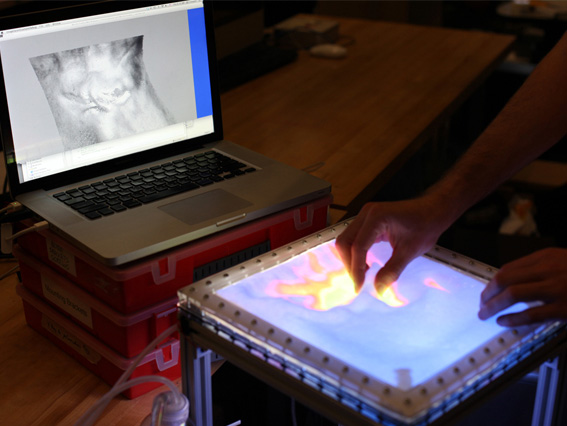
\includegraphics[width=\textwidth]{figures/jamming/jui_tunable-clay}
                \caption{Tuneable Clay}
                \label{fig:ch:jamming:jui-clay}
        \end{subfigure}
        \hspace{0.02\textwidth}
        \begin{subfigure}[b]{0.44\textwidth}
                \centering
                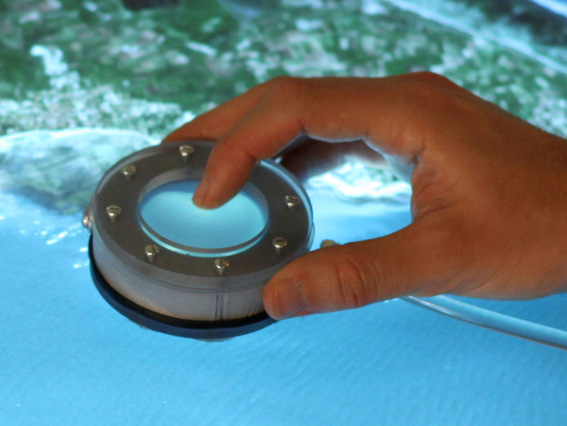
\includegraphics[width=\textwidth]{figures/jamming/jui_haptic-lens}
                \caption{Transparent Haptic Lens}
                \label{fig:ch:jamming:jui-lens}
        \end{subfigure}

        \begin{subfigure}[b]{0.44\textwidth}
                \centering
                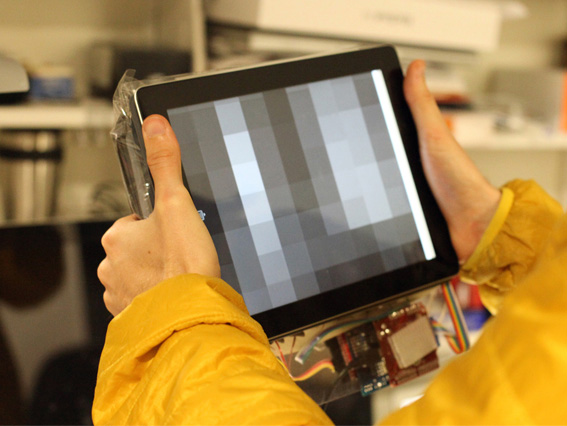
\includegraphics[width=\textwidth]{figures/jamming/jui_behind-the-tablet}
                \caption{Behind-the-Tablet Jamming}
                \label{fig:ch:jamming:jui-tablet}
        \end{subfigure}
        \hspace{0.02\textwidth}
        \begin{subfigure}[b]{0.44\textwidth}
                \centering
                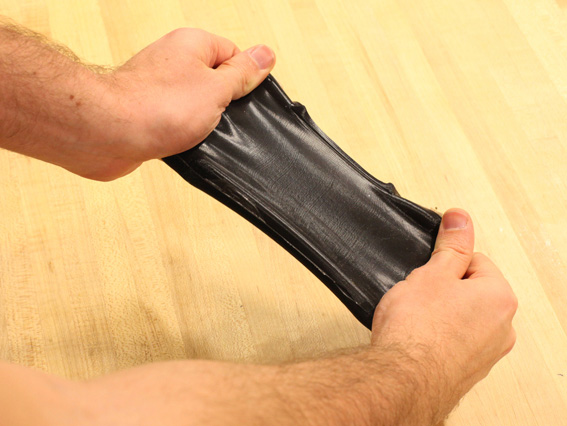
\includegraphics[width=\textwidth]{figures/jamming/jui_shapephone}
                \caption{ShapePhone}
                \label{fig:ch:jamming:jui-phone}
        \end{subfigure}
        \caption{Jamming User Interfaces by \citet{follmer2012jamming}.}
        \label{fig:ch:jamming:jui-collection}
\end{figure}

\subsection{Summary of related work}

In the previous sections we have given an introduction to the mechanics of jamming and an overview of different research applications of jamming.
These applications show two primary approaches to jamming.
The first one is the basic approach where a single volume containing particles can be jammed by applying a vacuum inside (see figure~\ref{fig:ch:jamming:approaches:basic}).
Applications of the basic approach are for example the \emph{Claytric Surface} and \emph{ShapePhone}.
The other is the more complicated cell-based approach where each cell is an independent jammable volume working in the same manner as the basic approach.
As the cells exist on the perimeter of the volume some other compound must constitute the body of the volume and stabilise the form.
In \emph{The HoverMesh} this was air inside a cubicle and in \emph{JSEL} it was fluid (see figure~\ref{fig:ch:jamming:approaches:cell}).

The related work demonstrate different potentials for the use of jamming through implementations based on mechanics, direct manipulation, shape-change, and as a feedback channel.
In table \ref{ch:jamming:table:applications_overview} we have summarises and categorises the mentioned applications according to their characteristics.
In the next section we will move on to our own concepts that support the notion of ad hoc interfaces.

\begin{landscape}
  \thispagestyle{empty}
  \centering 
  \captionof{table}{An overview and categorisation of related jamming work}
  \label{ch:jamming:table:applications_overview} 
  \begin{tabularx}{\linewidth}{|l|c|c|c|c|c|X|}
    \hline
    Project                 & Input                         & Output                        & Type      & Particles   & Approach  & Summary \\ \hline
    \hline
    Robotic gripper         & \cellcolor{FalseColor}\xmark  & \cellcolor{TrueColor}\cmark   & pneumatic & coffee      & basic     & A universal robotic gripper \\ \hline
    Jamming Skin Enabled Locomotion & \cellcolor{FalseColor}\xmark  & \cellcolor{TrueColor}\cmark   & pneumatic & glass beads     & cell-based& A soft moving robot \\ \hline
    Jamming Modulated Unimorph & \cellcolor{FalseColor}\xmark  & \cellcolor{TrueColor}\cmark   & pneumatic & glass beads          & cell-based& A worm-like robot \\ \hline
    \hline
    The HoverMesh           & \cellcolor{FalseColor}\xmark  & \cellcolor{TrueColor}\cmark   & pneumatic & polystyrene & cell-based& A cell-based deformable surface structure . \\ \hline    
    ClaytricSurface         & \cellcolor{TrueColor}\cmark   & \cellcolor{FalseColor}\xmark  & pneumatic & polystyrene & basic     & A flexible tabletop surface which serves as a sculptable display medium. \\ \hline
    Tunable Clay            & \cellcolor{TrueColor}\cmark   & \cellcolor{FalseColor}\xmark  & hydraulic & glass beads & basic     & A malleable tabletop for direct 3D modelling. \\ \hline
    Transparent Haptic Lens & \cellcolor{FalseColor}\xmark  & \cellcolor{TrueColor}\cmark   & hydraulic & glass beads & basic     & A small tangible puck to be used as a haptic information channel on a tabletop display. \\ \hline
    Behind-the-Tablet       & \cellcolor{TrueColor}\cmark   & \cellcolor{TrueColor}\cmark   & pneumatic & ?           & basic     & A tablet with a interactive jamming volume on the back. \\ \hline
    ShapePhone              & \cellcolor{TrueColor}\cmark   & \cellcolor{FalseColor}\xmark  & pneumatic & coffee      & basic     & a generic mobile device that can be shaped and locked into different forms. \\
    \hline
  \end{tabularx}

  \begin{flushleft}
  This table is an overview and categorisation of the prototypes presented in the papers covered in this section. It should be mentioned that in categorising \textit{input} and \textit{output} features we are only considering whether input or output is enabled using the jamming technique. For example, \textit{Tunable Clay} does have output in the form a image projection but it does not utilise the jamming technique.
  \end{flushleft}

\end{landscape}


\section{Exploring jamming concepts}
\label{ch:jamming:concepts} 
%!TEX root = ../thesis.tex
This section will focus on describing and discussing a selection of concepts for ad hoc interfaces based on the jamming technique.
As mentioned in the beginning of this chapter we were not successful at implementing a working jamming system where we could effectively control air/liquid flow.
Therefore we concentrate on conceptual prototypes which we envisioned before taking the decision to move in other directions.
Each of these concepts have different focal points.
The first one, \emph{\nameref{ch:jamming:concepts:dynamic_input}}, strives to achieve on-demand standard interfaces for input control.
The second, \emph{\nameref{ch:jamming:concepts:playful_blobs}}, seeks to draw on known interaction metaphors from the digital world and expose them to physical objects.
The third, \emph{\nameref{ch:jamming:concepts:improvised_furniture}}, scales up the dimensions and focuses on a living environment with highly configurable components.

\subsection{Dynamic input controls} 
\label{ch:jamming:concepts:dynamic_input}

This concept was our starting point for our first endeavours with jamming.

The concept resembles the work of \citet{harrison2009providing} mentioned in the related work section and our intentions were also to create physical input controls with the dynamic qualities of the digital counterpart.
But we were of the opinion that by using the jamming technique we could overcome some of the constraints of their approach and offer even more flexibility.
The limitations of the approach taken by \citet{harrison2009providing} were primarily the reliance on a backing layer where cut-out areas determined the position and shape of the buttons.
They were able to show a button either in convex or concave form or not at all, but the buttons were locked in their positions and the shapes were also not modifiable.

Instead, we propose using the jamming technique with a cell-based approach.
Individual cells can be used to create deformations on different areas of the surface and the composition of multiple cells makes it possible to make forms of heterogeneous shapes emerge anywhere on the plane, see figure \ref{fig:ch:jamming:concepts:button-cells}.
The idea of composition is quite similar to the that of computer graphics where polygons are used to compose images that are appear three-dimensional.
In this way, not only can we make input controls appear and disappear, we can also change the shape and position of them for an even more dynamic interface.

As a simple example we made mocked up a prototype to demonstrate simple shapes by jamming.
Due to our issues with a jamming, this was again a setup with a vacuum cleaner, plastic bag as the membrane, and ground coffee as the particles, see figure \ref{fig:ch:jamming:concepts:inputs-prototype}.

\begin{figure}[h]
  \centering
  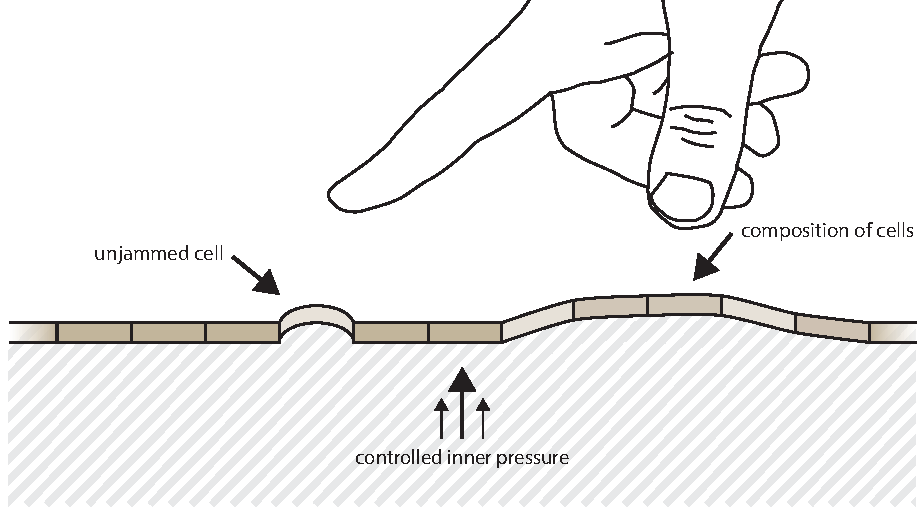
\includegraphics[width=.9\textwidth]{figures/jamming/concepts/jamming-inputs-concept.pdf}
  \caption{A cross-sectional view of a cell-based button and a composition multiple cells with different pressures for complex forms.}
  \label{fig:ch:jamming:concepts:button-cells}
\end{figure}

%We conceptualize on household appliances such as radios, clock alarms, house alarms heating, ventilation and air conditioning (HVAC), \todo{etc}.
%In general physical products with standard input controls such as buttons, knobs, switches and sliders.

\begin{figure}[h]
\centering
\begin{subfigure}[t]{.44\textwidth}
  \centering
  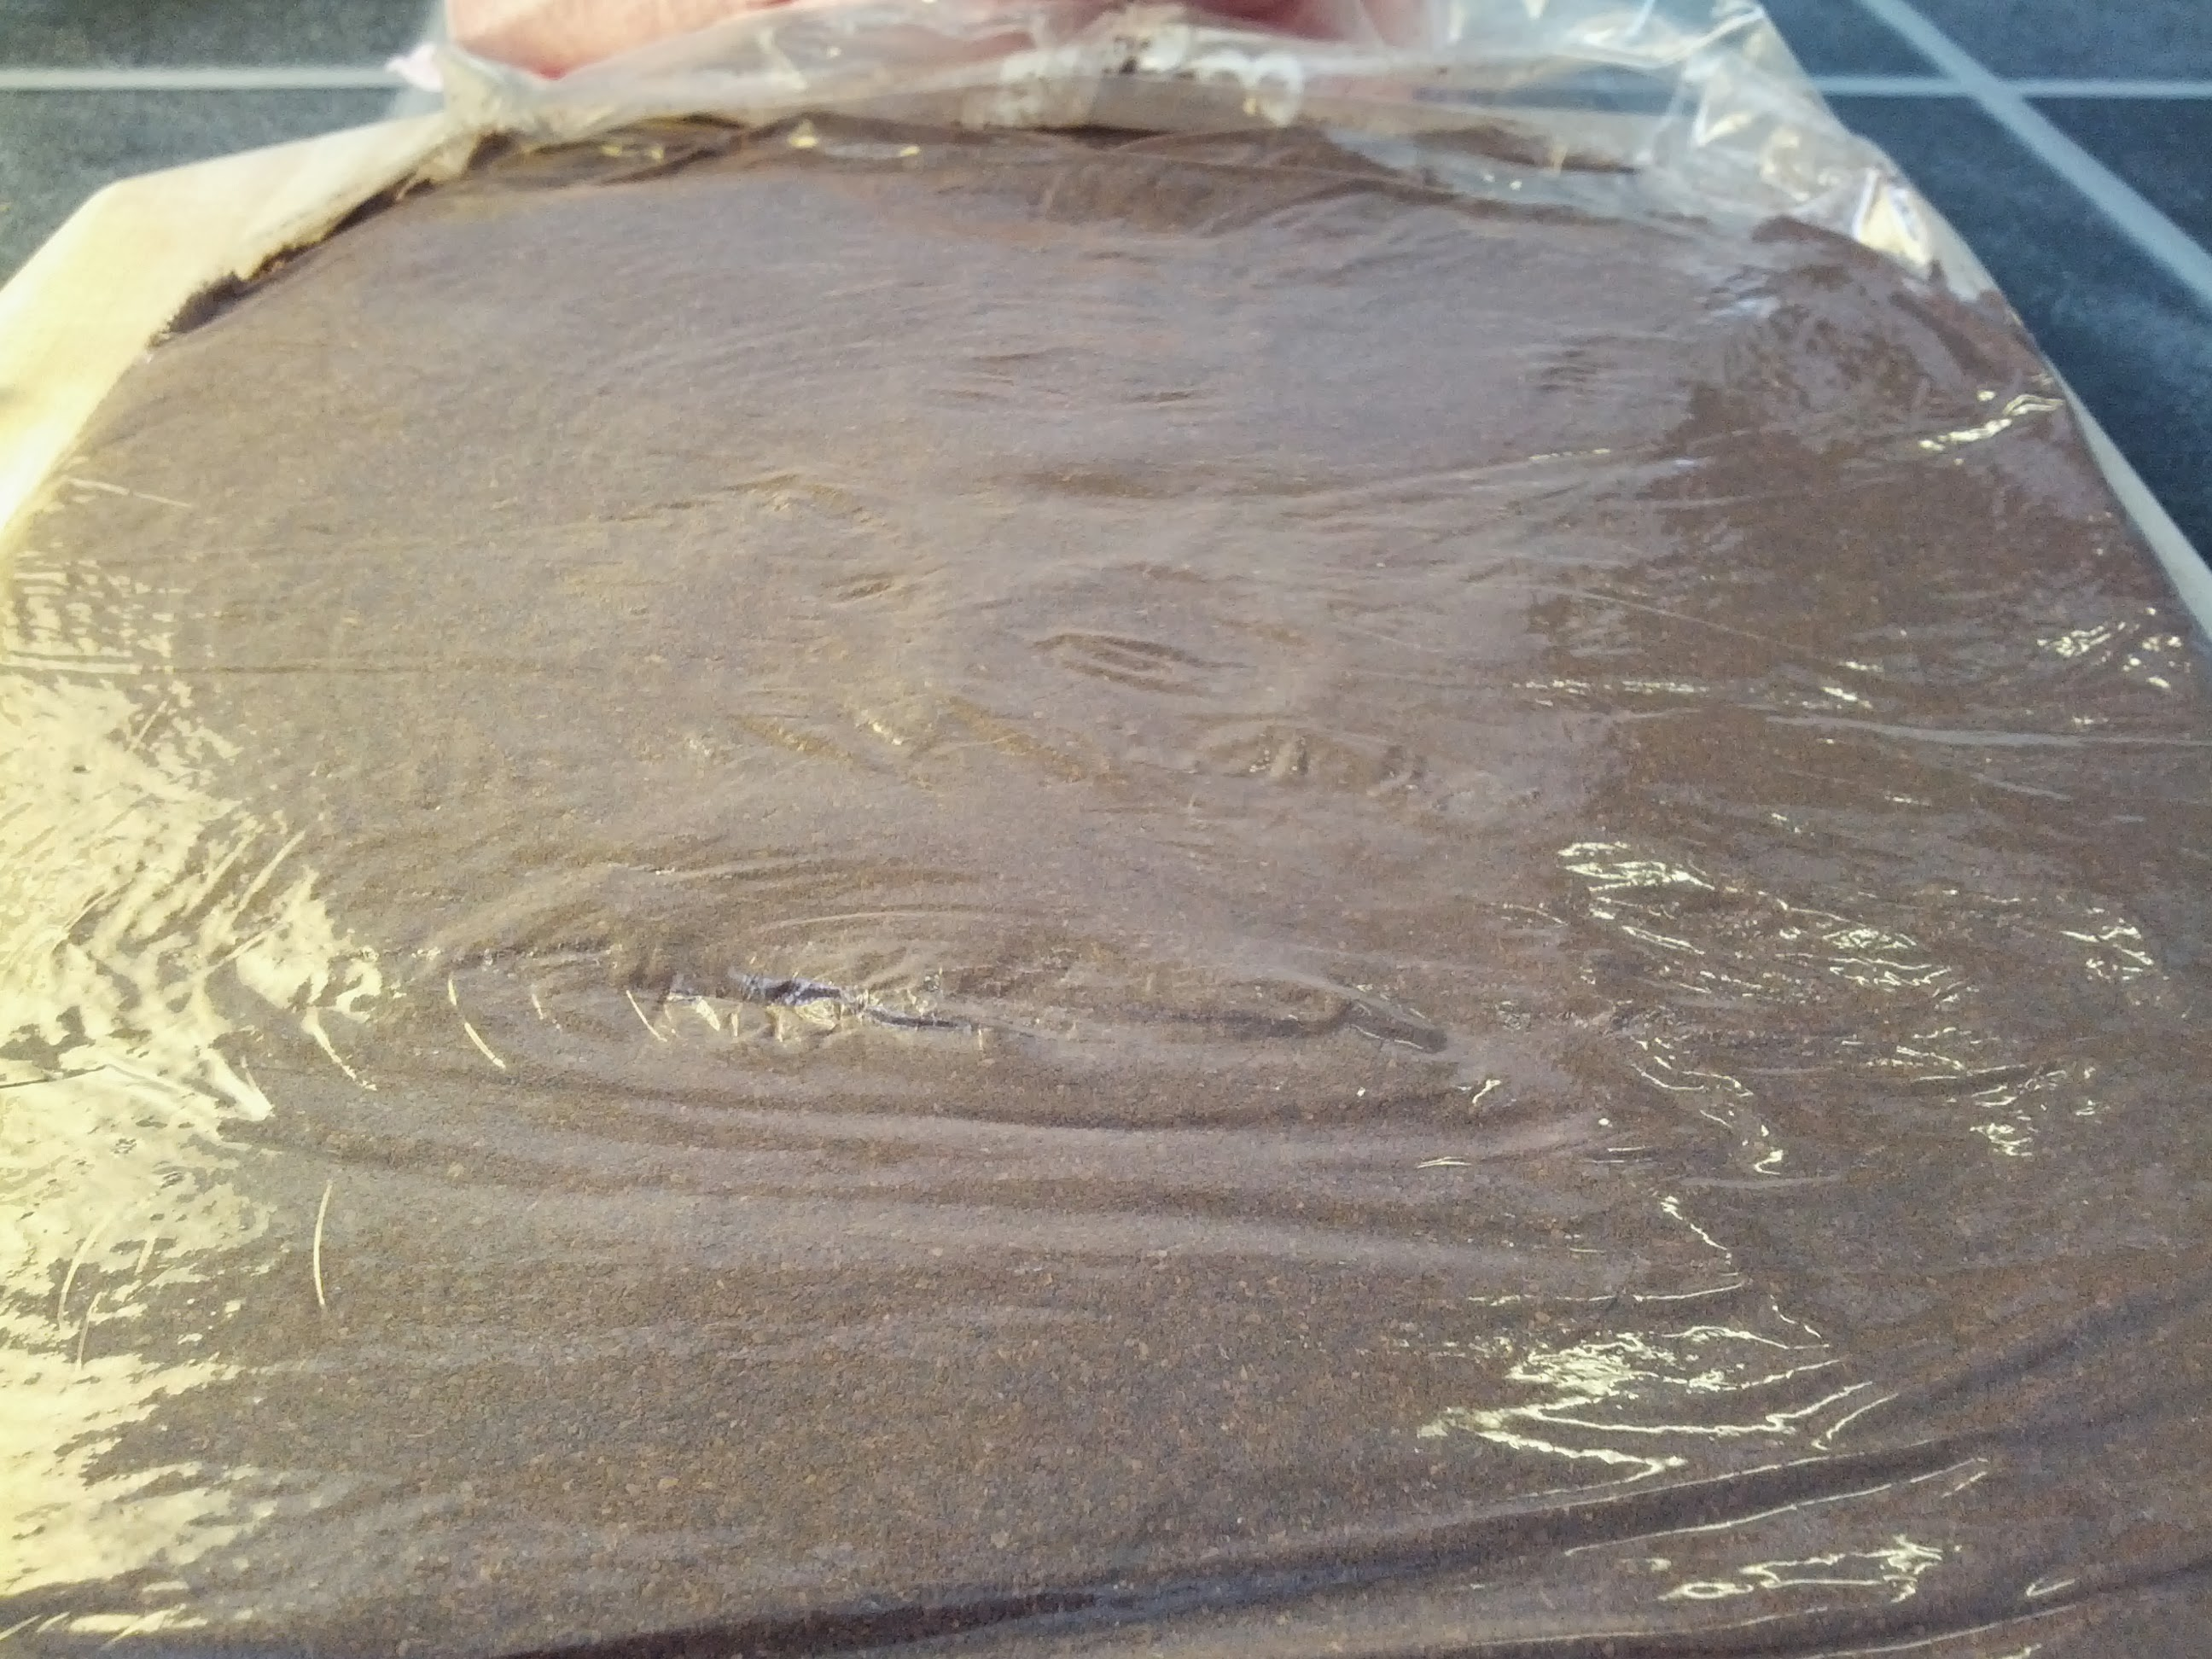
\includegraphics[width=\linewidth]{figures/jamming/concepts/inputs/jamming-inputs-flat}
    \caption{A flat surface with the absence of any input controls.}
\end{subfigure}%
\hspace{0.02\textwidth}
\begin{subfigure}[t]{.44\textwidth}
  \centering
  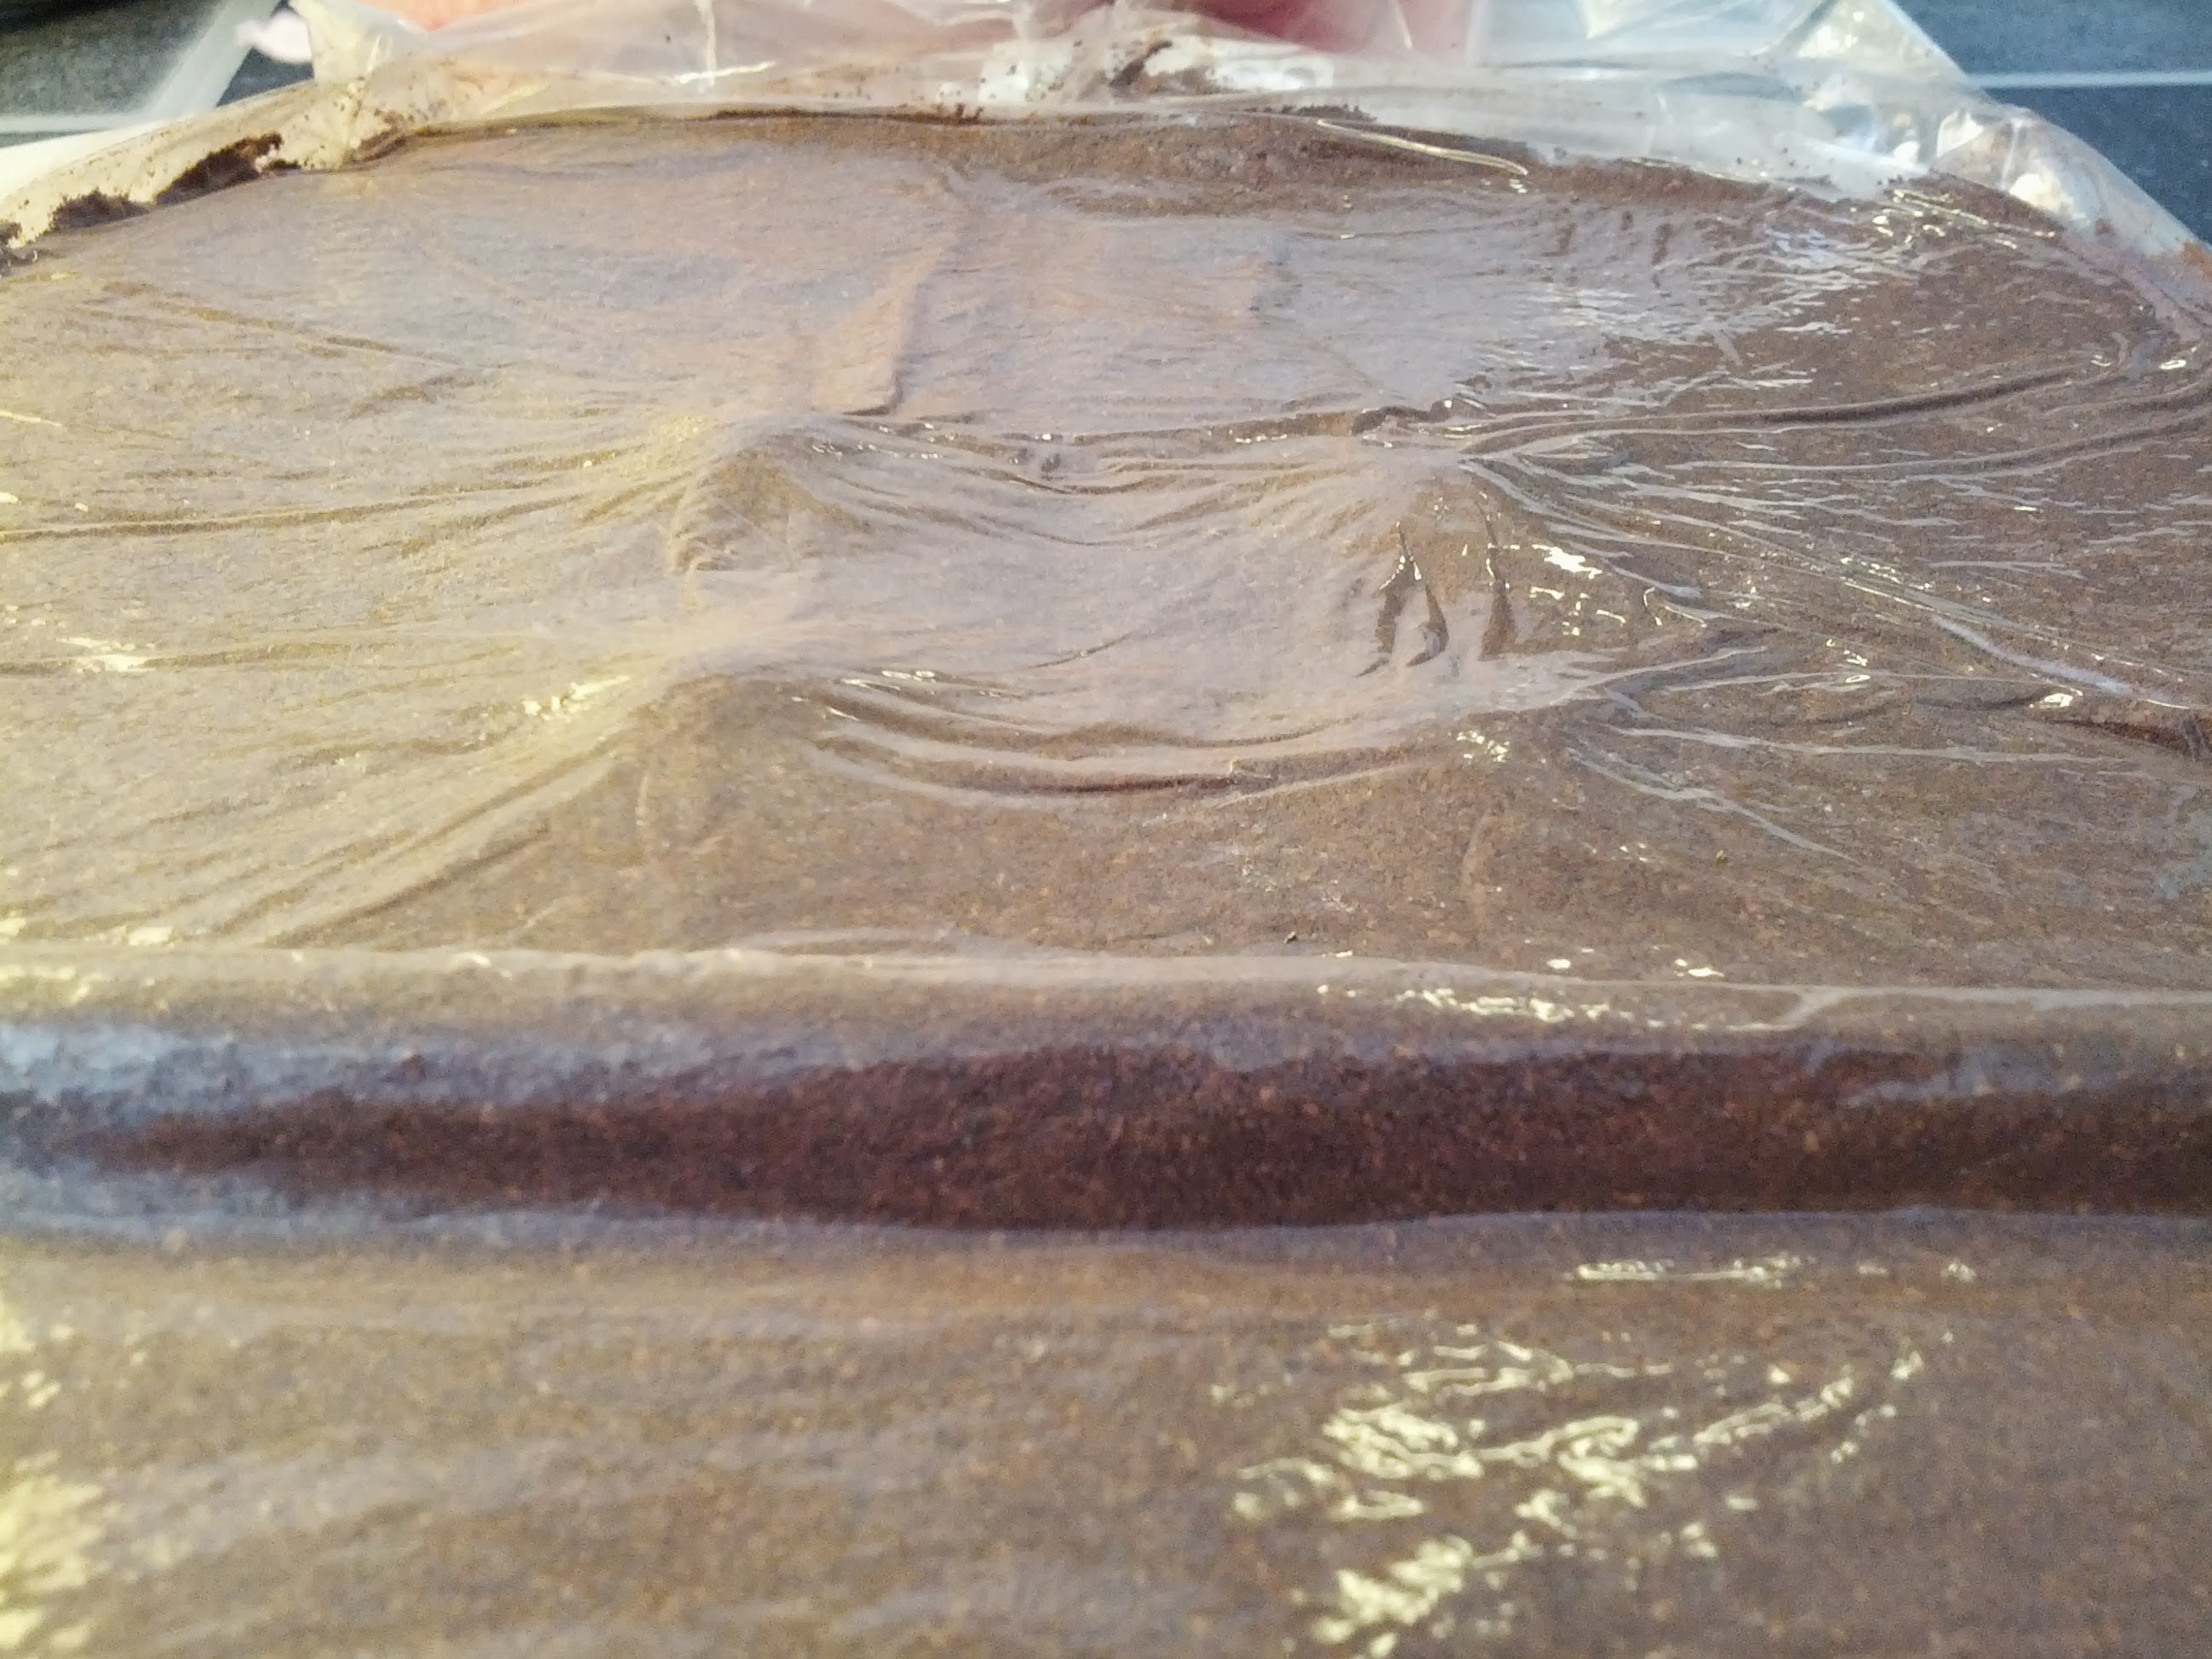
\includegraphics[width=\linewidth]{figures/jamming/concepts/inputs/jamming-inputs-buttons}
  \caption{Four buttons have emerged and an elongated input control for e.g. sliding or grabbing and pulling.}
\end{subfigure}
\caption{A primitive exploratory prototype with basic jamming of a single volume. Ground coffee is enclosed withing a transparent plastic bag. Wrinkles occur due to the plastic bag not being very flexible.}
\label{fig:ch:jamming:concepts:inputs-prototype}
\end{figure}

\subsection{Playful blobs}
\label{ch:jamming:concepts:playful_blobs}

The focal point of this next concept is on bringing input and output into the same object.
As can be seen in table~\ref{ch:jamming:table:applications_overview} on page~\pageref{ch:jamming:table:applications_overview} only one of the listed projects from the related work section, \nameref{fig:ch:jamming:jui-tablet}, has both input and output in same object.
Therefore we see an unexplored area of jamming potentials which we would like to address in the this next concept.

We envision a toy concept for children which we call \nameref{ch:jamming:concepts:playful_blobs}.
The blobs are tangible clay-like objects meant to be moulded into creative forms.
Each blob makes a selection of commands available otherwise known from digital interface metaphors, such as \emph{save, open, undo, delete, copy, and paste} which can actuate the blob in different ways.
These commands give a physical blob a notion of form memory where state is kept over time.
If needed previously saved forms can be recalled and further work on the form can done.
More specifically each command means (see also figure~\ref{fig:ch:jamming:concepts:blobs:states}):
\begin{itemize}
	\item{\emph{Save}: The current form of a blob is saved in memory for later retrieval.}
	\item{\emph{Open}: A previously saved form can be recalled and the blob actuates itself into the saved state.}
	\item{\emph{Undo}: Negate the latest moulding of the blob.}
	\item{\emph{Copy}: Make a copy of the state of a specific blob. The copied state could be saved in a blob or in an external object.}
	\item{\emph{Paste}: Set the state of a blob to that of which has been copied.} 
	\item{\emph{Delete}: Reset a blob so that all state is forgotten.} 
\end{itemize}

\begin{figure}[h]
  \centering
  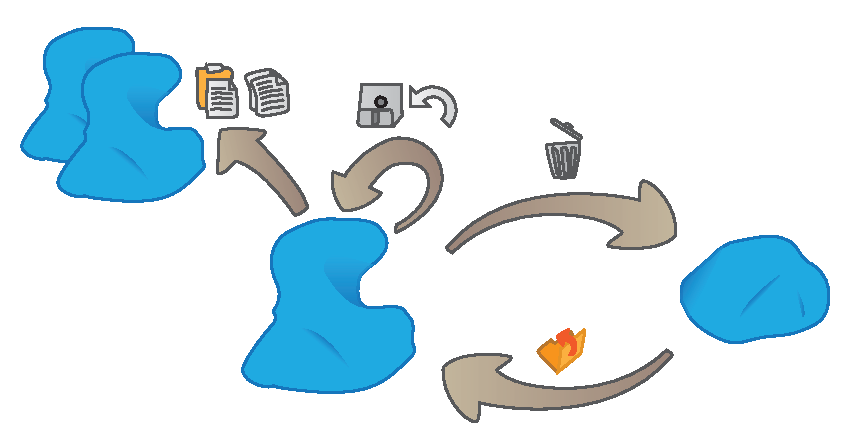
\includegraphics[width=.9\textwidth]{figures/jamming/concepts/blobs/state-transitions.pdf}
  \caption{A visualisation of the different commands and the associated state transititons.}
  \label{fig:ch:jamming:concepts:blobs:states}
\end{figure}

The commands are made possible via a cell-based jamming structure and the amount of detail a moulded blob can have is dictated by the resolution of the jamming cells.
As mentioned earlier this jamming approach makes it possible to separately control the stiffness of each cell.
So, for example, the \emph{save} command is done by storing a map of the current pressure states of each cell.
A subsequent \emph{open} or \emph{paste} command would set the correct pressure values of the cells and thereby restore the \emph{saved} or \emph{copied} physical form.
Lastly, a \emph{delete} command would release all negative pressure in cells and thereby collapse the form.
A simple prototype is shown figure~\ref{fig:ch:jamming:concepts:blobs:gloves} made with the basic jamming approach.
The actuation process would have to be done in a correct sequence in order for specific curvatures to become possible, which presumably could be done by computation.

\begin{figure}[h]
  \centering
  \begin{subfigure}[t]{.28\textwidth}
    \centering
    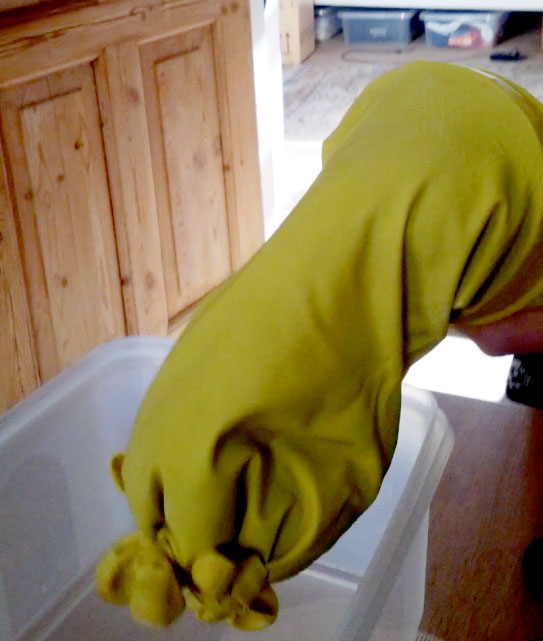
\includegraphics[width=\linewidth]{figures/jamming/concepts/blobs/glove-1.jpg}
    \captionof{figure}{The blob in collapsed state, i.e. no pressure is upheld.}
    \label{fig:ch:jamming:concepts:blobs:g1}
  \end{subfigure}%
  \hspace{0.03\textwidth}
  \begin{subfigure}[t]{.28\textwidth}
    \centering
    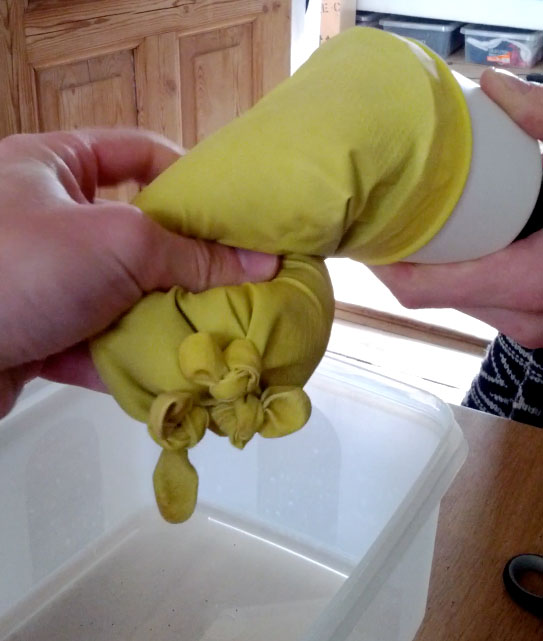
\includegraphics[width=\linewidth]{figures/jamming/concepts/blobs/glove-2}
    \captionof{figure}{The blob being molded into a custom shape.}
    \label{fig:ch:jamming:concepts:blobs:g2}
  \end{subfigure}
  \hspace{0.03\textwidth}
  \begin{subfigure}[t]{.28\textwidth}
    \centering
    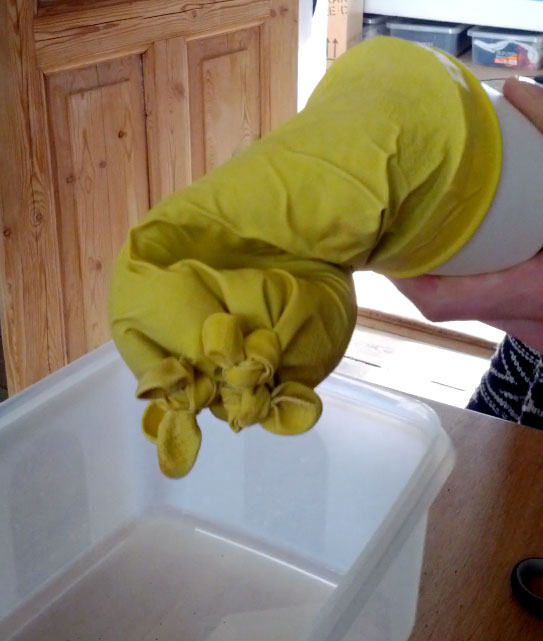
\includegraphics[width=\linewidth]{figures/jamming/concepts/blobs/glove-3}
    \captionof{figure}{The shape of the blob is maintained.} 
    \label{fig:ch:jamming:concepts:blobs:g3}
  \end{subfigure}
  \caption{An exploratory prototype of playful blobs. Created with a rubber latex glove, ground coffee, and a vacuum cleaner. For a video of the above steps see appendix~\ref{app:videos:jamming} which also shows the rigidity of the shape when jammed.}
  \label{fig:ch:jamming:concepts:blobs:gloves}
\end{figure}

We envision that the blobs can be used in a clay-like manner for kids to explore moulding of material into various forms and where particular interesting forms can be saved, duplicated and so on.
Furthermore, we also envision that these blobs could be used as the foundation for a new kind of dynamic building block for construction toys.
A concept that takes products such as Lego\footnote{http://www.lego.com/} a step further by having building blocks that are deformable and can be locked into any shape by the use of jamming.
This allows for block shapes that are no more limited to the supply of the production company but which allow for custom moulded blocks that are adapted to the needs of the user.

Applying these digital features to the physical blobs exhibits ad hoc qualities where the shape itself forms the interface and where shapes can be created on an ad hoc basis.
When a particular shape is no longer needed it can disappear again by remoulding it or letting it collapse (jamming-wise).

\subsection{Improvised furniture}
\label{ch:jamming:concepts:improvised_furniture}

This concept is based on replacing static components of the home with dynamic jamming enabled substitutes.
In its most extreme case with a large scale deployment it may be a little far fetched but an intriguing thought experiment and maybe not that unrealistic in a more futuristic scenario.
It underpins the idea of a configurable home where otherwise static and massive components such as walls and furniture allow for deformations.
For example, pushing in part of a wall to make room for a plant or even an entire shelf.
Or, deforming the floor to improvise an extra seat for a guest.
Or, adjusting the armrest or back of the sofa for a more comfortable position.

These examples correlate with what we touched upon in \autoref{ch:domain} about Steward Brands understanding of changes in a building;
Pulling down a given layer of change to a lower layer to create a more dynamic and adaptable environment.
The concept of improvised furniture would then be \emph{Space Plan} elements that are exposed to the layer of \emph{Stuff}. 
Figure~\ref{fig:ch:jamming:concepts:impro} illustrates deformation of walls for improvised furniture.

With this reconfigurability done by hand the components will naturally end up having an organic appearance with curvatures and very few straight lines and edges.

Using jamming in a large scale deployment where strength and bearing capacity is a requirement does come with quite a few constraints regarding materials.
The container of the particles must be strong enough to handle the exposed level of stress and strain while still being flexible enough to allow for surface deformations.

\begin{figure}[h]
  \centering
  \begin{subfigure}[t]{.44\textwidth}
    \centering
    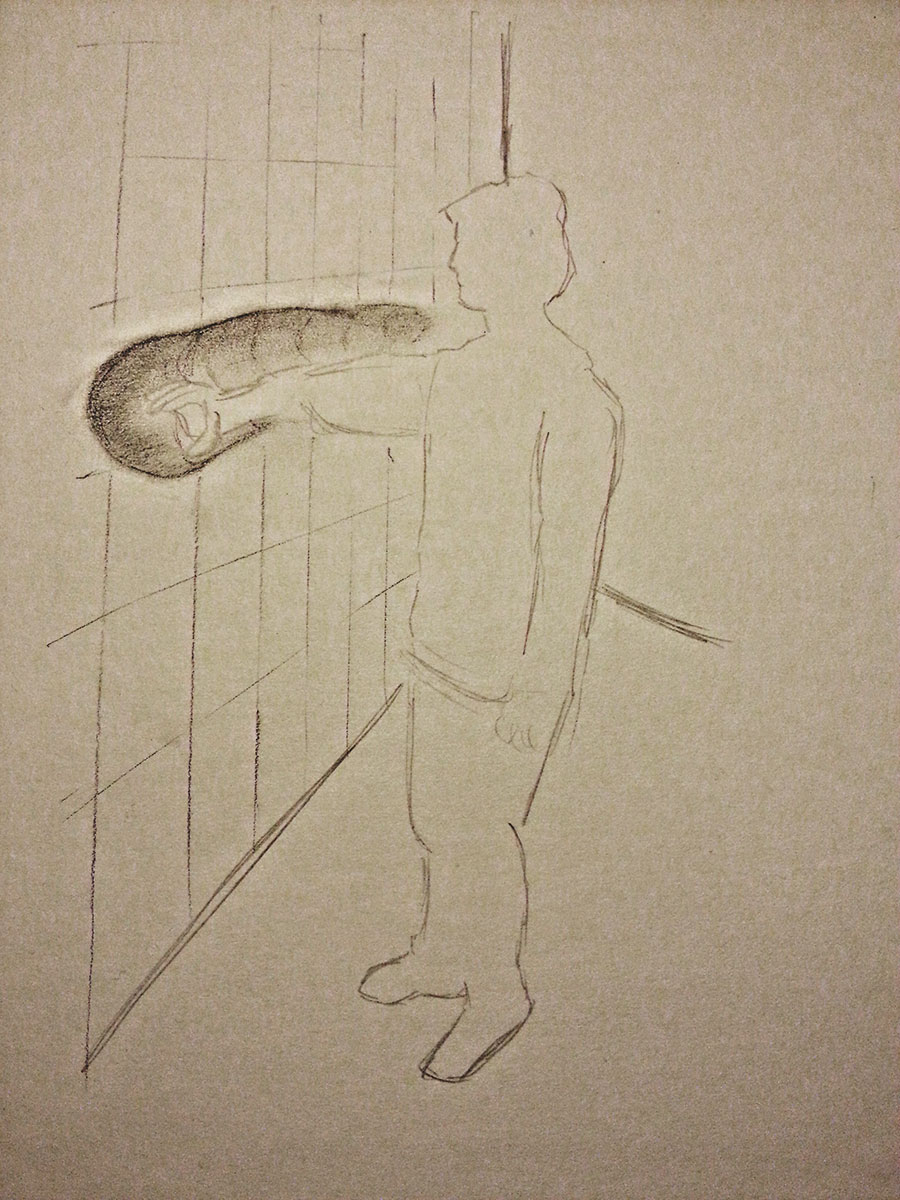
\includegraphics[width=\linewidth]{figures/jamming/concepts/impro/carve}
  \end{subfigure}%
  \hspace{0.02\textwidth}
  \begin{subfigure}[t]{.44\textwidth}
    \centering
    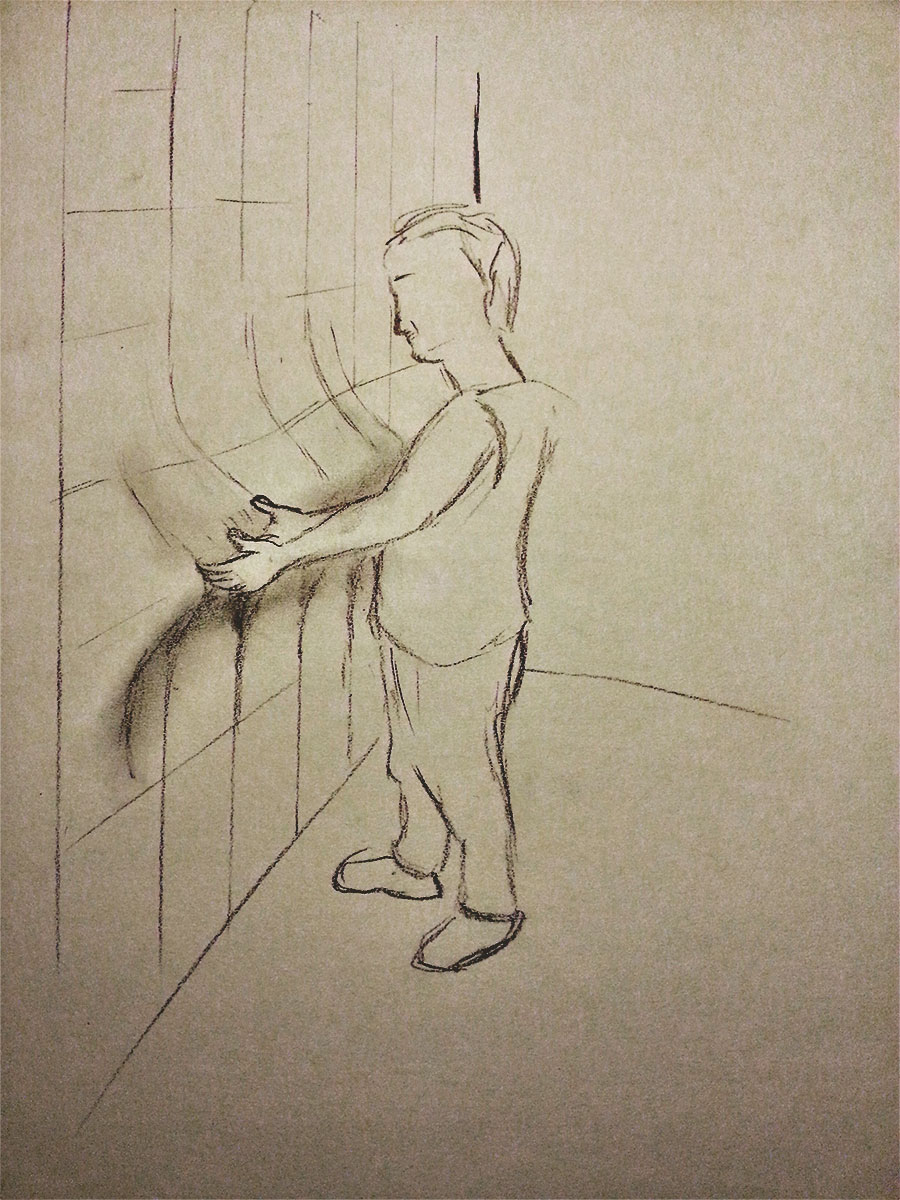
\includegraphics[width=\linewidth]{figures/jamming/concepts/impro/pull}
  \end{subfigure}
  \caption{Sketches of direct deformations of a wall by pushing and pulling, e.g. an improvised shelf.}
\label{fig:ch:jamming:concepts:impro}
\end{figure}



\section{Discussion}

As mentioned in the introduction working with SCIs is intrinsically complex and the jamming technique is no exception.
One thing that we do find convenient and positive about the technique is that is quite easy to make simple mock-up prototypes that do exhibit the shape-change qualities.
On top of that, these simple prototypes can be assembled from everyday household equipment such as coffee, plastic bags, cleaning gloves, balloons, vacuum cleaner, sticky tape, and other accessories.
In many ways this makes it straight forward to explore jamming qualities such as shape and viscosity change which gives a good insight to the potentials of jamming.
But when more sophisticated setups are needed, for instance cell-based jamming, and when the individual elements need to be controlled and interact in the right way, things get complicated.

Jamming allows for many of the types of shape-change categorised by \citet{rasmussen2012shape}.
In its simplest form, namely basic jamming (cf. figure~\ref{fig:ch:jamming:approaches:basic}) viscosity, texture and form are the primary types of shape-change possible with jamming.
But when the technique is combined with other means of actuation that can affect the jamming volume (cf. cell-based jamming in figure~\ref{fig:ch:jamming:approaches:cell}) the types of shape-change possible are expanded to include volume and orientation (as output) as well as accentuating the primary types.
Other types such as spatiality and the non-topological types adding/subtracting and permeability are not directly possible with jamming as the technique requires a bounded and non-perforated volume to function.

\citet{follmer2012jamming} demonstrated that jamming also has the potential for providing rich user feedback. 
Haptic feedback through stiffness control (viscosity) was presented in the projects Transparent Haptic Lens and Behind-The-Tablet.
These examples were both done with basic jamming volumes which shows that it is a simple and straight-forward approach to this kind of haptic feedback compared to a mechanical alternative.

\section{Conclusions}
In this chapter we have introduced jamming as an enabling technology for shape changing interfaces and explained the mechanics of particle jamming.
The current range of research projects with jamming within mechanical engineering and HCI has been covered.
Though the number of jamming-related contributions are few, promising applications and potentials have been presented.
In any case, we are certain that the contributions from researchers such as \citet{follmer2012jamming} and \citet{matoba2012claytricsurface} are not the last we have seen of the jamming technique within HCI.

Our own explorations with the jamming technique has resulted in three concepts that address the first of three approaches to constructing ad hoc interfaces, which we presented in \autoref{ch:adhoc:defining-ahi}:
\begin{enumerate}
	\item{\emph{Using shape change as the construction mechanism.}}
\end{enumerate}
The first concept, \emph{\nameref{ch:jamming:concepts:dynamic_input}}, was an exploration of dynamic and flexible interfaces for input controls, such as buttons, sliders, and knobs.
The second, \emph{\nameref{ch:jamming:concepts:playful_blobs}}, looked into physical objects with digital qualities which could change shape to fit a specific purpose, be it for clay-like moulding or as dynamic building blocks.
The third concept, \emph{\nameref{ch:jamming:concepts:improvised_furniture}}, explored the concept of highly configurable home where otherwise static components allow of surface deformation.
The explorations that we have presented in this chapter underpin the potential for jamming, and shape-change in general, as a valid approach for ad hoc interfaces where physical malleability supports the dynamic nature of AHIs.


\chapter{Prototyping: Textile Touch}
\label{ch:textile-touch}
%!TEX root = thesis.tex
Our second prototype will move away from the world of jammable shape changing interfaces and into the surfaces of our environment.
In this chapter we will take a look at our second construction approach that we suggest for AHIs in chapter~\ref{ch:adhoc} where AHIs are embedded into the surfaces of our environment, ready to emerge when the user has a need for it.

Since the vision of ubiquitous computing was presented researchers have sought to integrate interactive technology into our everyday environment in variety of ways, which can be seen from the diverse selection of research fields that has stemmed from ubiquitous computing such as context awareness, tangible computing and shape changing interfaces.
In this prototype we have taken Weiser's vision very literally - how do you integrate interaction into the fabric of our everyday environment, i.e. the surfaces that surrounds us?

In the following sections we explore the possibilities of creating textile touch surfaces with advanced interaction capabilities as an exemplification of how surfaces can be used to interact in the home to create ad hoc interaction.
We have chosen to work with textiles as an interactive platform as we see unused potential in this area, both for its tangible and aesthetic textural qualities compared to e.g. polymer solutions \cite{rosenberg2009unmousepad}, as well as for the interesting possibilities to allow for DIY solutions to creating interactive surfaces in the home.

The prototype that we have made for this chapter serves to exemplify both the qualities and possibilities of textile interfaces in general but also as an example of how surfaces in our environment can be enhanced and used in new ways for ad hoc interaction.

\todo{helt kort om hvad vi specifikt har lavet}

\section{Related work and approaches}
Before getting into detail with our implementation we will first give an overview of work and approaches that relates to our prototype and have inspired our solution.
We are, of course, not the first ones to consider the surfaces that surrounds us as interactive potential.
For example interactive floors such as iFloor \citep{petersen2005floor} and  iGameFloor \citep{gronbaek2007igamefloor}, augmented surface displays in fridges, walls and bowls \citep{taylor2007homes}, interactive tables such as reacTable \citep{jorda2007reactable} or, quite different from the other examples, REVEL that via a digital overlay changes the tactile perception of a physical surfaces \citep{bau2013revel}.

We have separated this section into three different fields that all have influenced the construction and implementation of our prototype work: electronic textiles, touch sensing and gesture recognition.
 
\subsection{Electronic Textiles}
\label{ch:textiletouch:related:etextiles}
\begin{quotation}
\emph{The most profound technologies are those that disappear. They weave themselves into the fabric of everyday life until they are indistinguishable from it. \citep{weiser1991computer}}
\end{quotation}
One of the research areas that have stemmed from ubiquitous computing is electronic textiles or `e-textiles', which seeks to integrate electronic and computation into fabric.
\citet{park2002wearable} presents the E-Textile vision as the paradigm the ``fabric is the computer'', taking Weiser's much quoted description of ubiquitous computing very literal.
One of the main obstacles for attaining this vision of the \emph{fabric as the computer} is how to incorporate the underlying computation into the fabric.
There are generally seen three ways to do it, either by computing \emph{offline}, on a separate system connected to the fabric, \emph{onto}, on components attached to the fabric or \emph{into} the fabric, embedded seamlessly into it \citep{marculescu2003}.
Today computation is commonly done either offline or onto the fabric, or a combination of the two, but advances in organic electronics and nano technology, for example with organic transistors weaved into fabric \citep{lee2005weave}, suggests that computation embedded into the fabric is not far off.

\begin{figure}[h]
\centering
\begin{minipage}[b]{.3\textwidth}
  \centering
  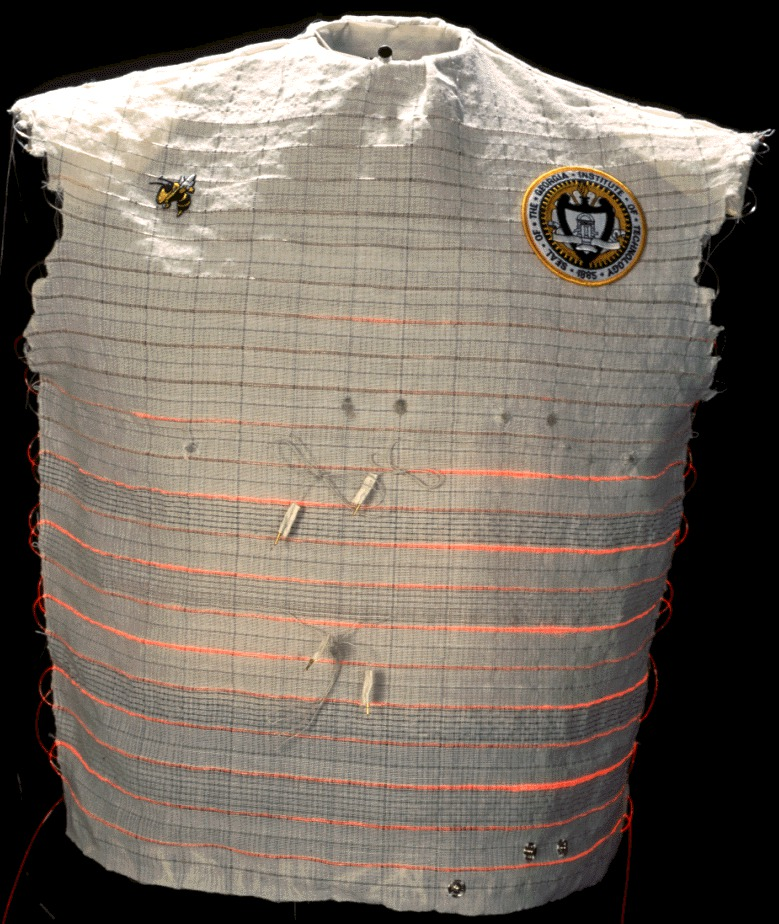
\includegraphics[width=0.9\linewidth]{figures/wearable_motherboard}
  \captionof{figure}{The Wearable Motherboard, from \citep{gopalsamy1999wearable}}
  \label{sofa_interaction:wearable_motherboard}
\end{minipage}%
\hspace{0.2cm}
\begin{minipage}[b]{.3\textwidth}
  \centering
  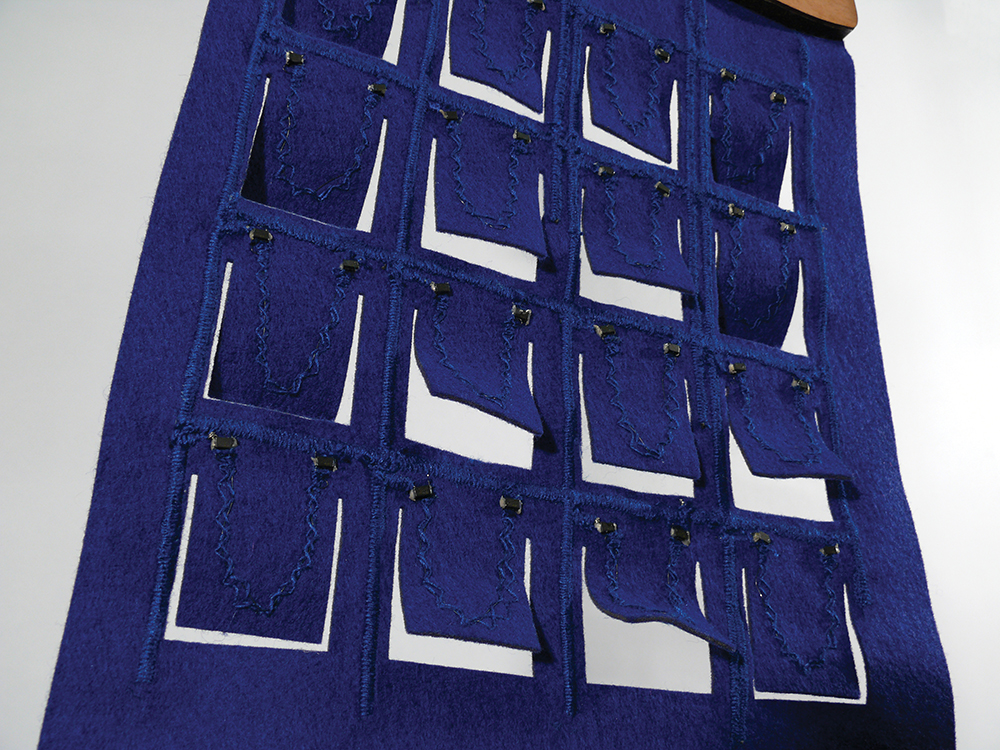
\includegraphics[width=0.9\linewidth]{figures/shutters}
  \captionof{figure}{Shutters, from \citep{coelho2009shutters}}
  \label{sofa_interaction:shutters}
\end{minipage}
\hspace{0.2cm}
\begin{minipage}[b]{.3\textwidth}
  \centering
  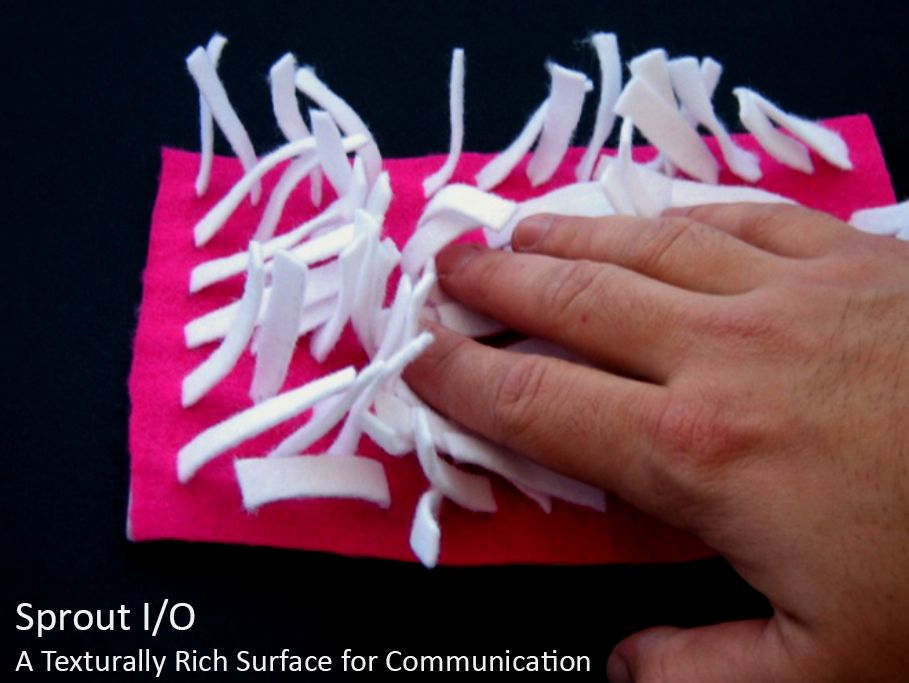
\includegraphics[width=0.9\linewidth]{figures/sprout}
  \captionof{figure}{Sprout I/O, from \citep{coelho2009shutters}}
  \label{sofa_interaction:sprout}
\end{minipage}
\end{figure}
E-textile is often seen used as part of wearable computing systems, logically, since clothing as a medium is ever present when people are involved.
An example of this is the Wearable Motherboard \citep{gopalsamy1999wearable} seen in figure~\ref{sofa_interaction:wearable_motherboard}, also called the ``Smart Shirt'', which is a lightweight monitoring `shirt' that can provide sensory data for use in medical and military contexts.
The fabric here is used as data paths that facilitates routing of information from any point to any other point on the shirt through conductive fibers embedded in the fabric.

E-textiles are not limited to wearable computing and clothing, and can just as well be part of interior design such as curtains, pillows, carpets, upholstery ect.
Shutters by \citet{coelho2009shutters}, seen in figure~\ref{sofa_interaction:shutters}, is an example of this where shape-memory alloy (SMA) threads are woven into a felt surface creating a curtain-like structure capable change of shape in permeability, used for indoor ventilation control among other things.
Here the SMA allows for actuation in the shutters while retaining the look, feel and softness of textile without any hard mechanic actuators.  
Another example from \citet{coelho2008sprout} is Sprout I/O, see figure~\ref{sofa_interaction:sprout}, where a membrane filled with strands of SMA and felt provides textually rich input and actuated output capabilities.
By measuring the capacitance between the users hand and the SMA threads touches can be registered, enabling stroke-like interaction, by creating an input matrix that register changes in each of the the individual SMA threads.

We have gotten a lot of inspiration from the various ``Do It Yourself'' (DIY) on-line communities related to e-textile craft and crafts in general, notably KOBAKANT DIY\footnote{http://www.kobakant.at/DIY/} and Instructable\footnote{http://www.instructables.com/}.
Both sites provides guides, tips, and tricks for materials, construction and techniques and have for us been a good starting point for doing an e-textile project.
One of our inspirations has been rSkin\footnote{http://www.plusea.at/?p=2255 and http://www.instructables.com/id/rSkin-Open-Source-Robot-Skin/}, a project by Hannah Perner-Wilson, which attempts to create a `skin' for a robot arm, made out of textiles, that enables the arm to register intensity and location of touches on the whole arm, seen in figure~\ref{rskin}.

\begin{figure}[h]
	\centering
  		\includegraphics[width=3in]{figures/rskin}
	\caption{rSkin, Open Source Robot Skin}
   \label{rskin}
\end{figure}
The `skin' is made of stretchy fabric and a 28 rows x 28 columns large pressure sensitive grid is embedded into the fabric using conductive thread.
The skin is made out of three layers: first a non-conductive layer with 28 rows of conductive thread, then a layer piezoresistive fabric and lastly a non-conductive layer with 28 columns of conductive thread.
The piezoresistive fabric acts as a pressure sensitive layer, as piezoresistive materials decrease their electrical resistivity under mechanical stress\footnote{http://en.wikipedia.org/wiki/Piezoresistive\_effect}.
This approach to making pressure sensitive grids will be described in further detail in the implementation section as we use it as a starting point for our second prototype iteration.

\subsection{Touch Sensing}
\label{ch:textiletouch:related:touch}
\todo{bedre indledning}

Generally seen there are three broad categories for doing multi-touch input sensing: optical, capacitive and resistive \citep{rosenberg2009unmousepad}.

Optical sensing usually involve one or more digital cameras placed behind the touch surface to generate an image of the user's finger to track the interaction.
As this approach relies on cameras it is typically used for larger applications such as tabletops, since the cameras has to be far enough away to capture entire interactive surface, e.g. reacTable \citep{jorda2007reactable}, seen in figure~\ref{sofa_interaction:reactable} and the tabletop version of Microsoft Surface.

Capacitive sensing systems for touch based interaction rely on the human body's capacitive abilities to acquire the position of the touch on a surface. 
As a finger touches the surface, the surface's electrostatic field distorts and this change is then measurable as a change in capacitance at some position in a 2D grid.
The most common example of this approach is the touch surface of modern smart phones and tablets where touch has become the preferred form of interaction, for example Apples iPad seen in figure~\ref{sofa_interaction:ipad}.
Another example is Touch\'e \citep{sato2012touche} that allow objects and environments to become touch sensitive, allowing everyday objects to become touch interfaces, such as doorhandles, cups, water bottles ect.
This is done by sending a signal through the object and doing electromagnetic frequency sweeps. 
These frequencies will change when a touch occur and will change based on the size of the touched on the surface allowing for simple gesture recognition.
Two limitations of this technology is that pressure can not reliably be measured and that most systems based this technology only works with bare skin touching it.    

Resistive sensing is based on the principle of Force Sensitive Resistance (FSR).
The basic principle of a FSR sensor is to apply current to a semi-conductive material with piezoresistive capabilities then and measure the voltage drop through the material.
As stress is applied to the semi-conductor the resistance will decrease and as a result the voltage will drop less. 
\citet{rosenberg2009unmousepad} describes FSR devices as 
\begin{quotation}
\emph{a continuous electrical switch through which electric conductance increases gradually as external force is applied}
\end{quotation}
The simple approach to making a touch sensetive surface, with multiple input areas, is to create a discrete array of FSR sensors in which each sensor has its own input and output channel.
This has some obvious limitations that will be discussed in iteration 1 in the next section.
Another approach is to create a row/column grid as seen in previously mentioned rSkin, this approach will be explored in iteration 2.
Lastly in iteration 3 we will explore the approach suggested by \citet{rosenberg2009unmousepad} to create a device based on IFSR, which is interpolating FSR, to increase the resolution of our prototype.
Generally seen resistive sensing is a low-cost and easy to implement solution to doing multi-touch interfaces and has the added benefit of being able to measure pressure.
It does also enable the use of flexible materials such as polymers in UnMousePad, seen wrapped on a coffee cup in figure~\ref{sofa_interaction:unmousepad}, and fabrics, as seen in rSkin where it is wrapped on a robot arm in figure~\ref{rskin}.
Though to attain resolutions higher than the size of the underlying grid, a lot of data processing has to be done as seen in \citep{rosenberg2009unmousepad}.
Also from our own experience with the technology we have seen a lot of input signal noise from the sensor which makes it harder to get accurate position tracking.   

\begin{figure}[h]
  \centering
  \begin{subfigure}[b]{.3\textwidth}
    \centering
    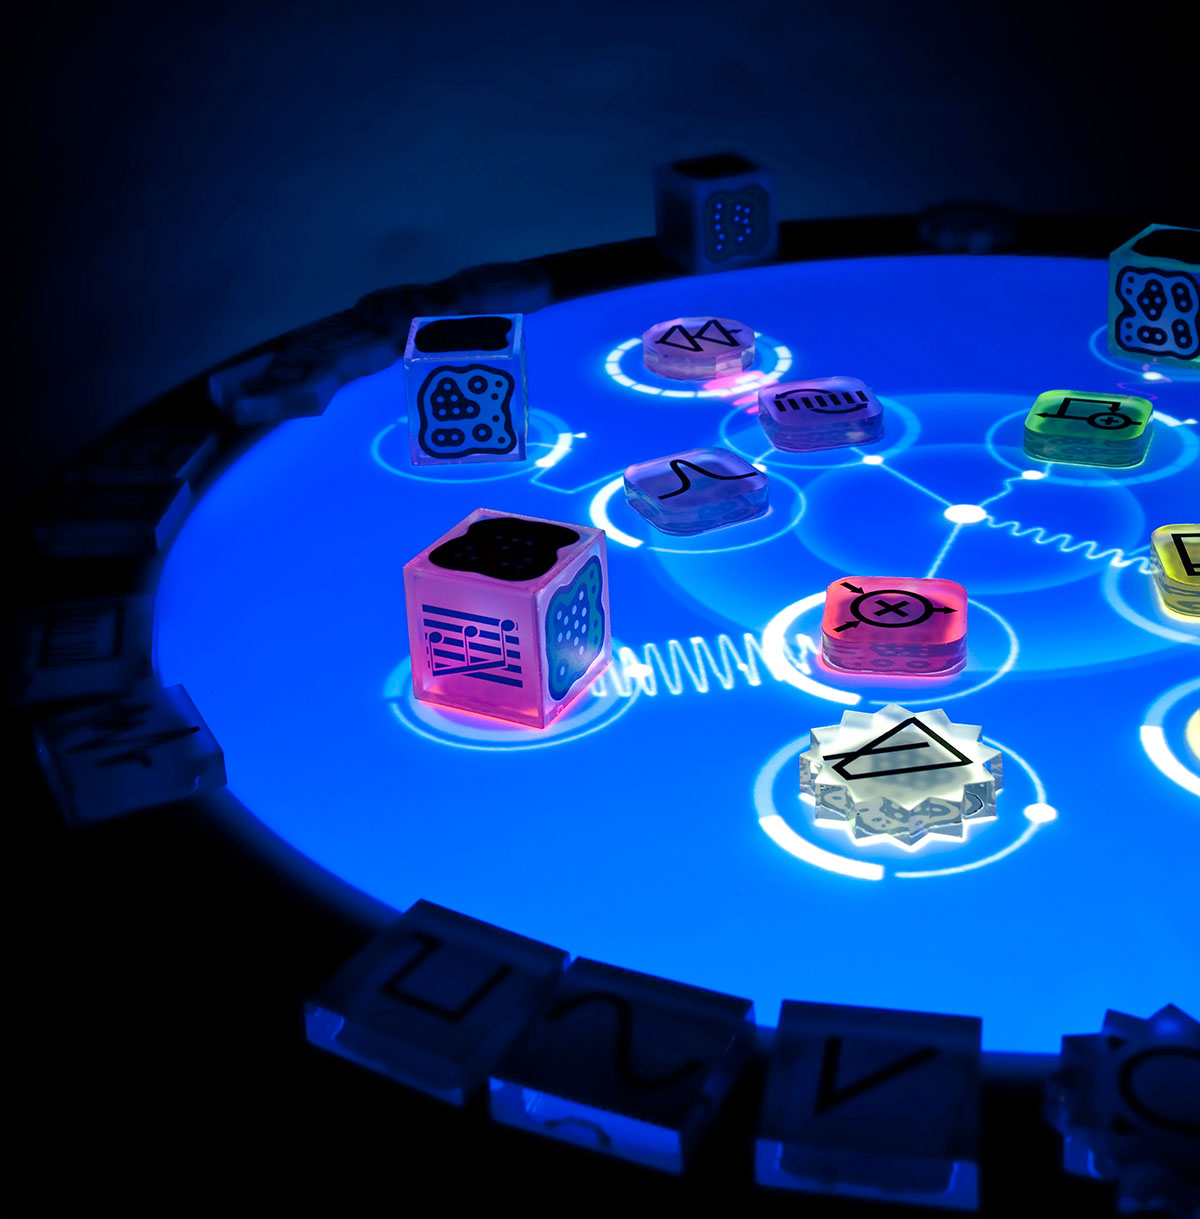
\includegraphics[width=0.9\linewidth]{figures/touch/reactable}
    \captionof{figure}{Optical sensing, reacTable}
    \label{sofa_interaction:reactable}
  \end{subfigure}%
  \hspace{0.2cm}
  \begin{subfigure}[b]{.3\textwidth}
    \centering
    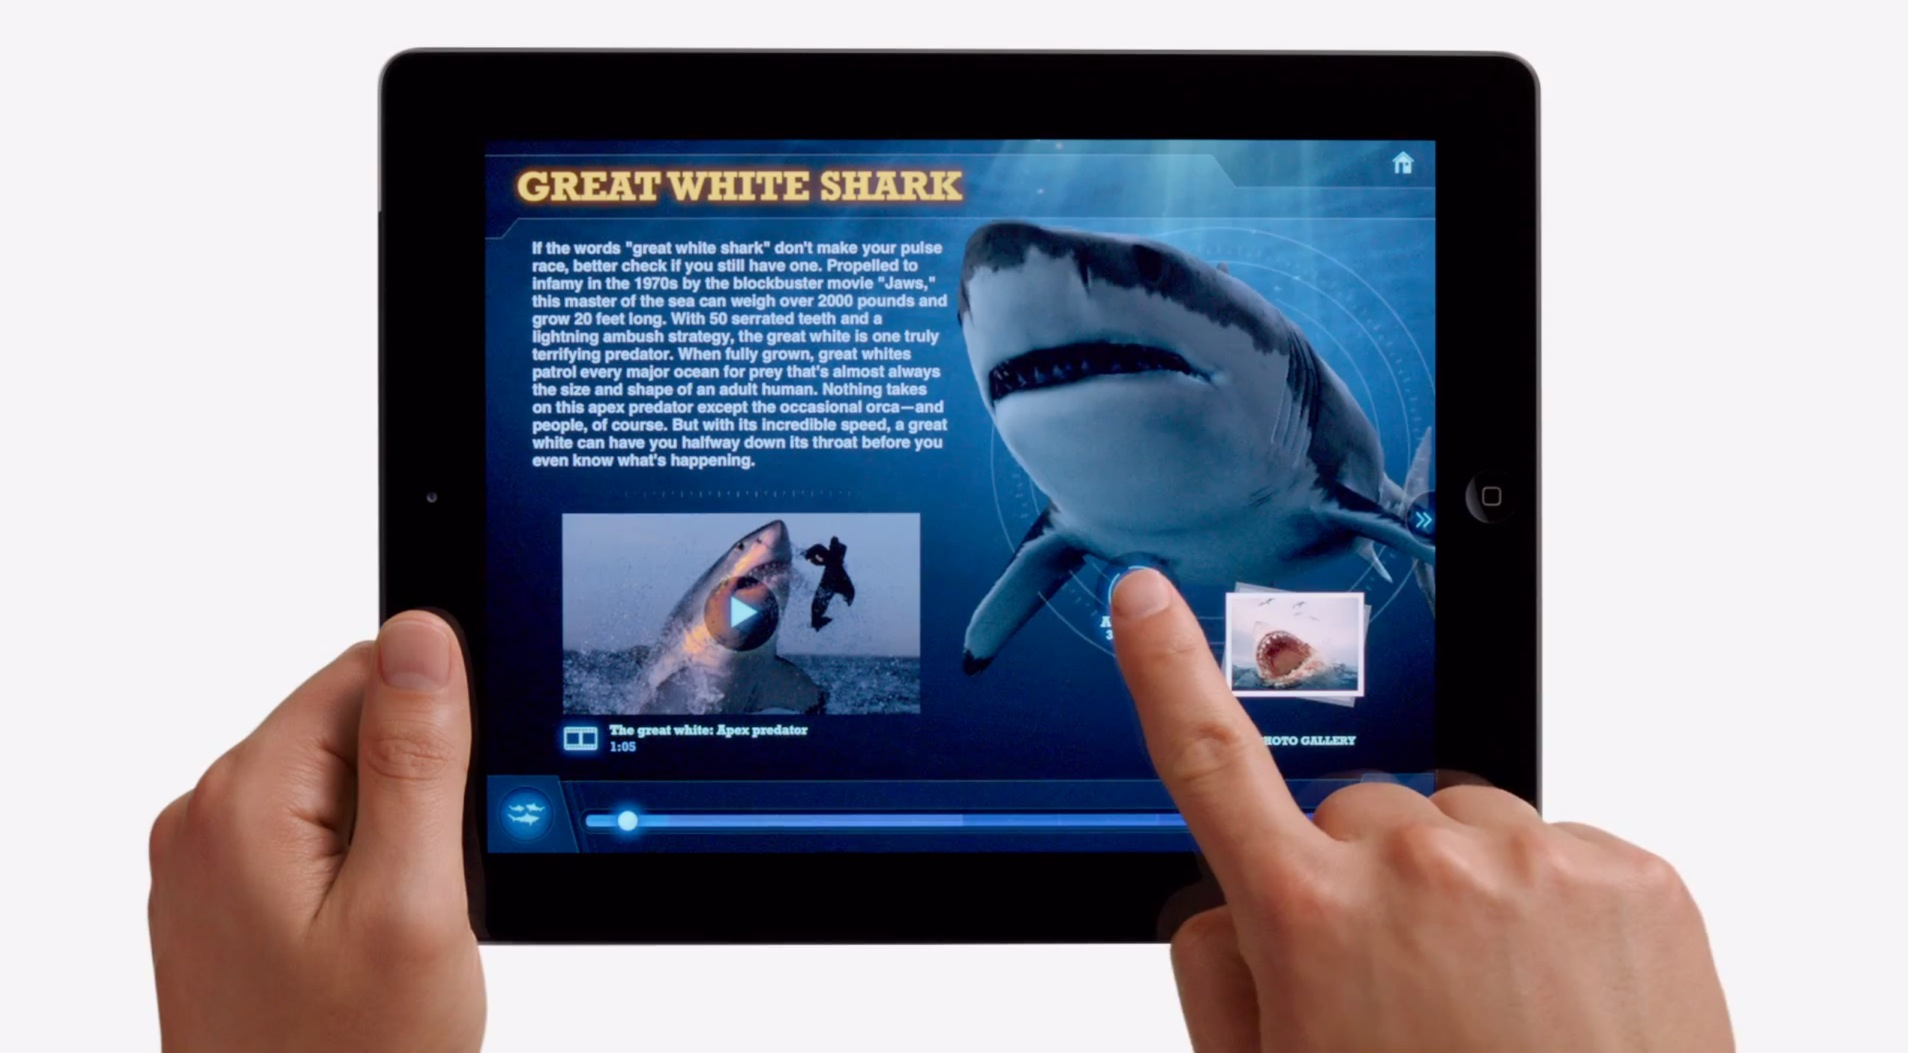
\includegraphics[width=0.9\linewidth]{figures/touch/ipad}
    \captionof{figure}{Capacitive sensing, iPad}
    \label{sofa_interaction:ipad}
  \end{subfigure}
  \hspace{0.2cm}
  \begin{subfigure}[b]{.3\textwidth}
    \centering
    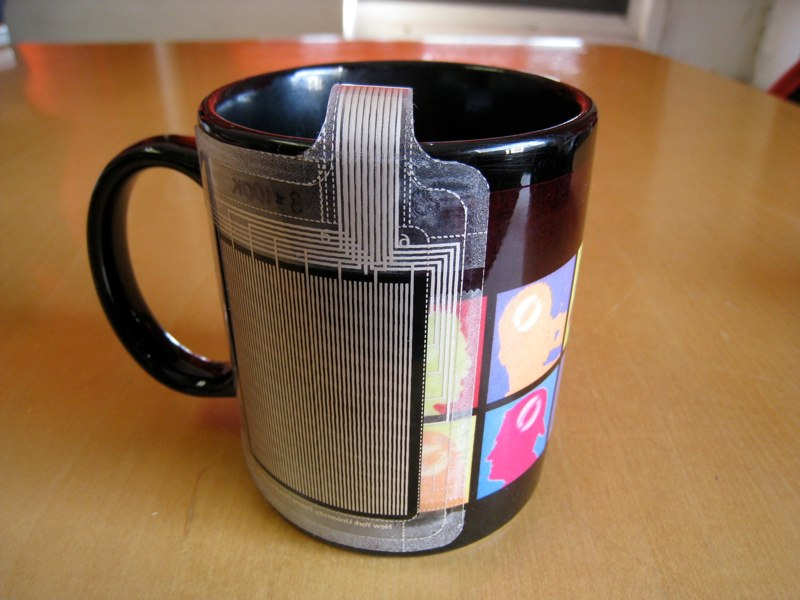
\includegraphics[width=0.9\linewidth]{figures/touch/unmousepad}
    \captionof{figure}{Resistive sensing, UnMousePad} 
    \label{sofa_interaction:unmousepad}
  \end{subfigure}
  \caption{Examples of different sensing systems.}
  \label{sofa_interaction:sensing_systems}
\end{figure}

\subsection{Gesture recognition}
\label{ch:textiletouch:gesture_recognition}
Being able to sense a x-y position or a pressure map on an interactive surface is usually not enough for an application to provide interesting interaction possibilities.
Adding gestures can be one way to approach the interaction in a more involving, natural and expressive way.
\citet{baudel1993charade} points out three possible advantages in using gesture based systems:
\begin{itemize}
  \item \emph{Natural interaction:} Gestures are a natural and intuitive way to interact that is easy to learn.
  \item \emph{Terse and powerful interaction:} The expressive nature of a gesture can provide the ability for a single gesture to specify both a command and its parameters.
  \item \emph{Direct interaction:} As the hand is used for input no intermediate transducer is needed
\end{itemize}
Gestures inherent expressive character does pose a challenge though as the computer system has to interpret the gesture in some way to give it meaning.
Reversely the user needs to know, or at least have hints at, which gestures that the system understands in order to interact with it.
Some types of gestures and their interaction meaning has eventually become so common that their behaviour is expected when interacting with touch interfaces today, for example pinch for zoom out, inverse pinch for zoom in and horizontal swipes for shifting though pages.
A standardized interaction model for gesture interfaces are still a long way off though, at least in our opinion. 

The increase in mainstream use of touch input devices of various types and sizes such as tablets, tabletops and smart phones has resulted in some easily accessible frameworks for doing gesture recognition.
This is a relatively new thing as earlier gesture recognition was reserved for experts in pattern matching and therefore not quite suitable for user interface prototyping, unless you where able to put a large amount of work into it \citep{wobbrock2007gestures}.  

\todo{mere om dollar recognizers generelt}

The dollar family of recognizers \citep{anthony2010lightweight,vatavu2012gestures,wobbrock2007gestures} are some of the most popular frameworks for doing easily implementable 2-D gesture recognition.
This family of recognizers are all geometric template matchers which means that they match the user input against a predefined template, and based on an Euclidean distance scoring function, selects the best match between template and input.
\begin{itemize}
  \item \emph{\$1-recognizer \citep{wobbrock2007gestures}:} is a single-stroke recognizer, fast
  \item \emph{\$N-recognizer \citep{anthony2010lightweight}:} is a multi-stroke recognizer, slow
  \item \emph{\$P-recognizer \citep{vatavu2012gestures}:} is a single and multi-stroke point-cloud recognizer, faster than \$N
\end{itemize}
We have implemented and experimented with the \$N and \$P recognizer as to determine which one performs the best with our data input, this will be discussed in \nameref{ch:textiletouch:gesture_implementation} in \ref{ch:textiletouch:gesture_implementation}.

\todo{giver det mening at teste dollar-1?}

\section{Concept (el. Design Principles som i Coelho)}
%!TEX root = ../thesis.tex
The prototype that we have made for this chapter serves to exemplify both the qualities and possibilities of textile interfaces in general but also as an example of how surfaces in our environment can be enhanced and used in new ways for ad hoc interaction.
Our prototype is a generic touch surface meant to be integrated into the environment in various ways.
As the prototype has been made with textiles it is most suitable for textile based integrations such as furniture, sheets, cloth etc.
The technique used does however extend beyond the use of textiles and could just as well be implemented with other materials such as wallpaper, polymers, or printed circuit boards (PCB).

To explore more advanced touch interactions the prototype is programmed to recognise various gestures which we exemplify by a scenario of controlling existing devices of the home.
These gestures are then mapped to \todo{mangler noget}

%The scenarios which we have envisioned are focus around pervasive touch surfaces in the home environment for the control of existing devices.

\section{(Process and) Implementation}
%!TEX root = ../thesis.tex
This section will go though the process and implementation of our prototype.
\todo{As one of the goals of this prototype has been to implement advanced interaction possibilities into a textile surface without the use of advanced machinery ... something something}
To give an insight into the prototype process as well as the final prototype, we have chosen to split the implementation into three overall iteration steps.
Our hope is that this will give a better understanding of the rationale behind our construction decisions as well as ... something something 

\todo{iterationer skal indeholder motivation for n\ae ste skridt \dots}

\todo{iteration 1 is longer because we describes the basics osv. ??}

\subsection{Iteration 1}
\label{ch:textiletouch:it1}
The goal of our first iteration of the prototype was to ensure that the we had construction principles and the right materials for constructing a touch and pressure sensitive fabric, with only off-the-shelf materials and tools.

\subsubsection{Construction principles}
As a first iteration of our prototype we applied the principles from Pressure Sensor Matrix\footnote{http://www.instructables.com/id/Pressure-Sensor-Matrix/}, to construct a simple 2x3 touch pad in neoprene, seen in figure~\ref{prototype_1}, and a bend sensor for simple testing, also seen in figure~\ref{prototype_1}.
The prototype consists of three layers as depicted in figure~\todo{ref}, connected to an Arduino\footnote{http://www.arduino.cc/} for input/output data that is sent to Processing\footnote{http://processing.org/} for data visualization.

\begin{figure}[h]
  \centering
      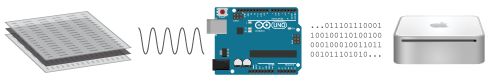
\includegraphics[width=\textwidth]{figures/touch/process}
  \caption{Data process}
   \label{data-process}
\end{figure}

The top layer is made of 3 mm thick neoprene from an old mouse pad with one long conductive thread, made of stainless steel fibers, sewn into it.
Neoprene is easy to work with and gives a natural force-feedback when touched because of its thickness, \hl{but lacks the naturalness and flexibility of normal fabric used for clothing}.
The middle layer made from anti-static polymer bags that are normally used to protect electronics. 
Some types of anti-static bags, such as the ones we have used, acts as semi-conductors with piezoresistive capabilities and therefore fits in a FSR sensor.
We have tested three different types of anti-static bags, two  transparent and one black, but only black ones are piezoresistive.
We do not know if this is the general case as we only had a limited number of samples.
The bottom layer is another layer of neoprene, but with separate conductive stitchings for each of the 2 x 3 cells.
The setup is illustrated in figure~\ref{layers_iteration1}.

\begin{figure}[h]
\centering
\begin{subfigure}[t]{.5\textwidth}
  \centering
  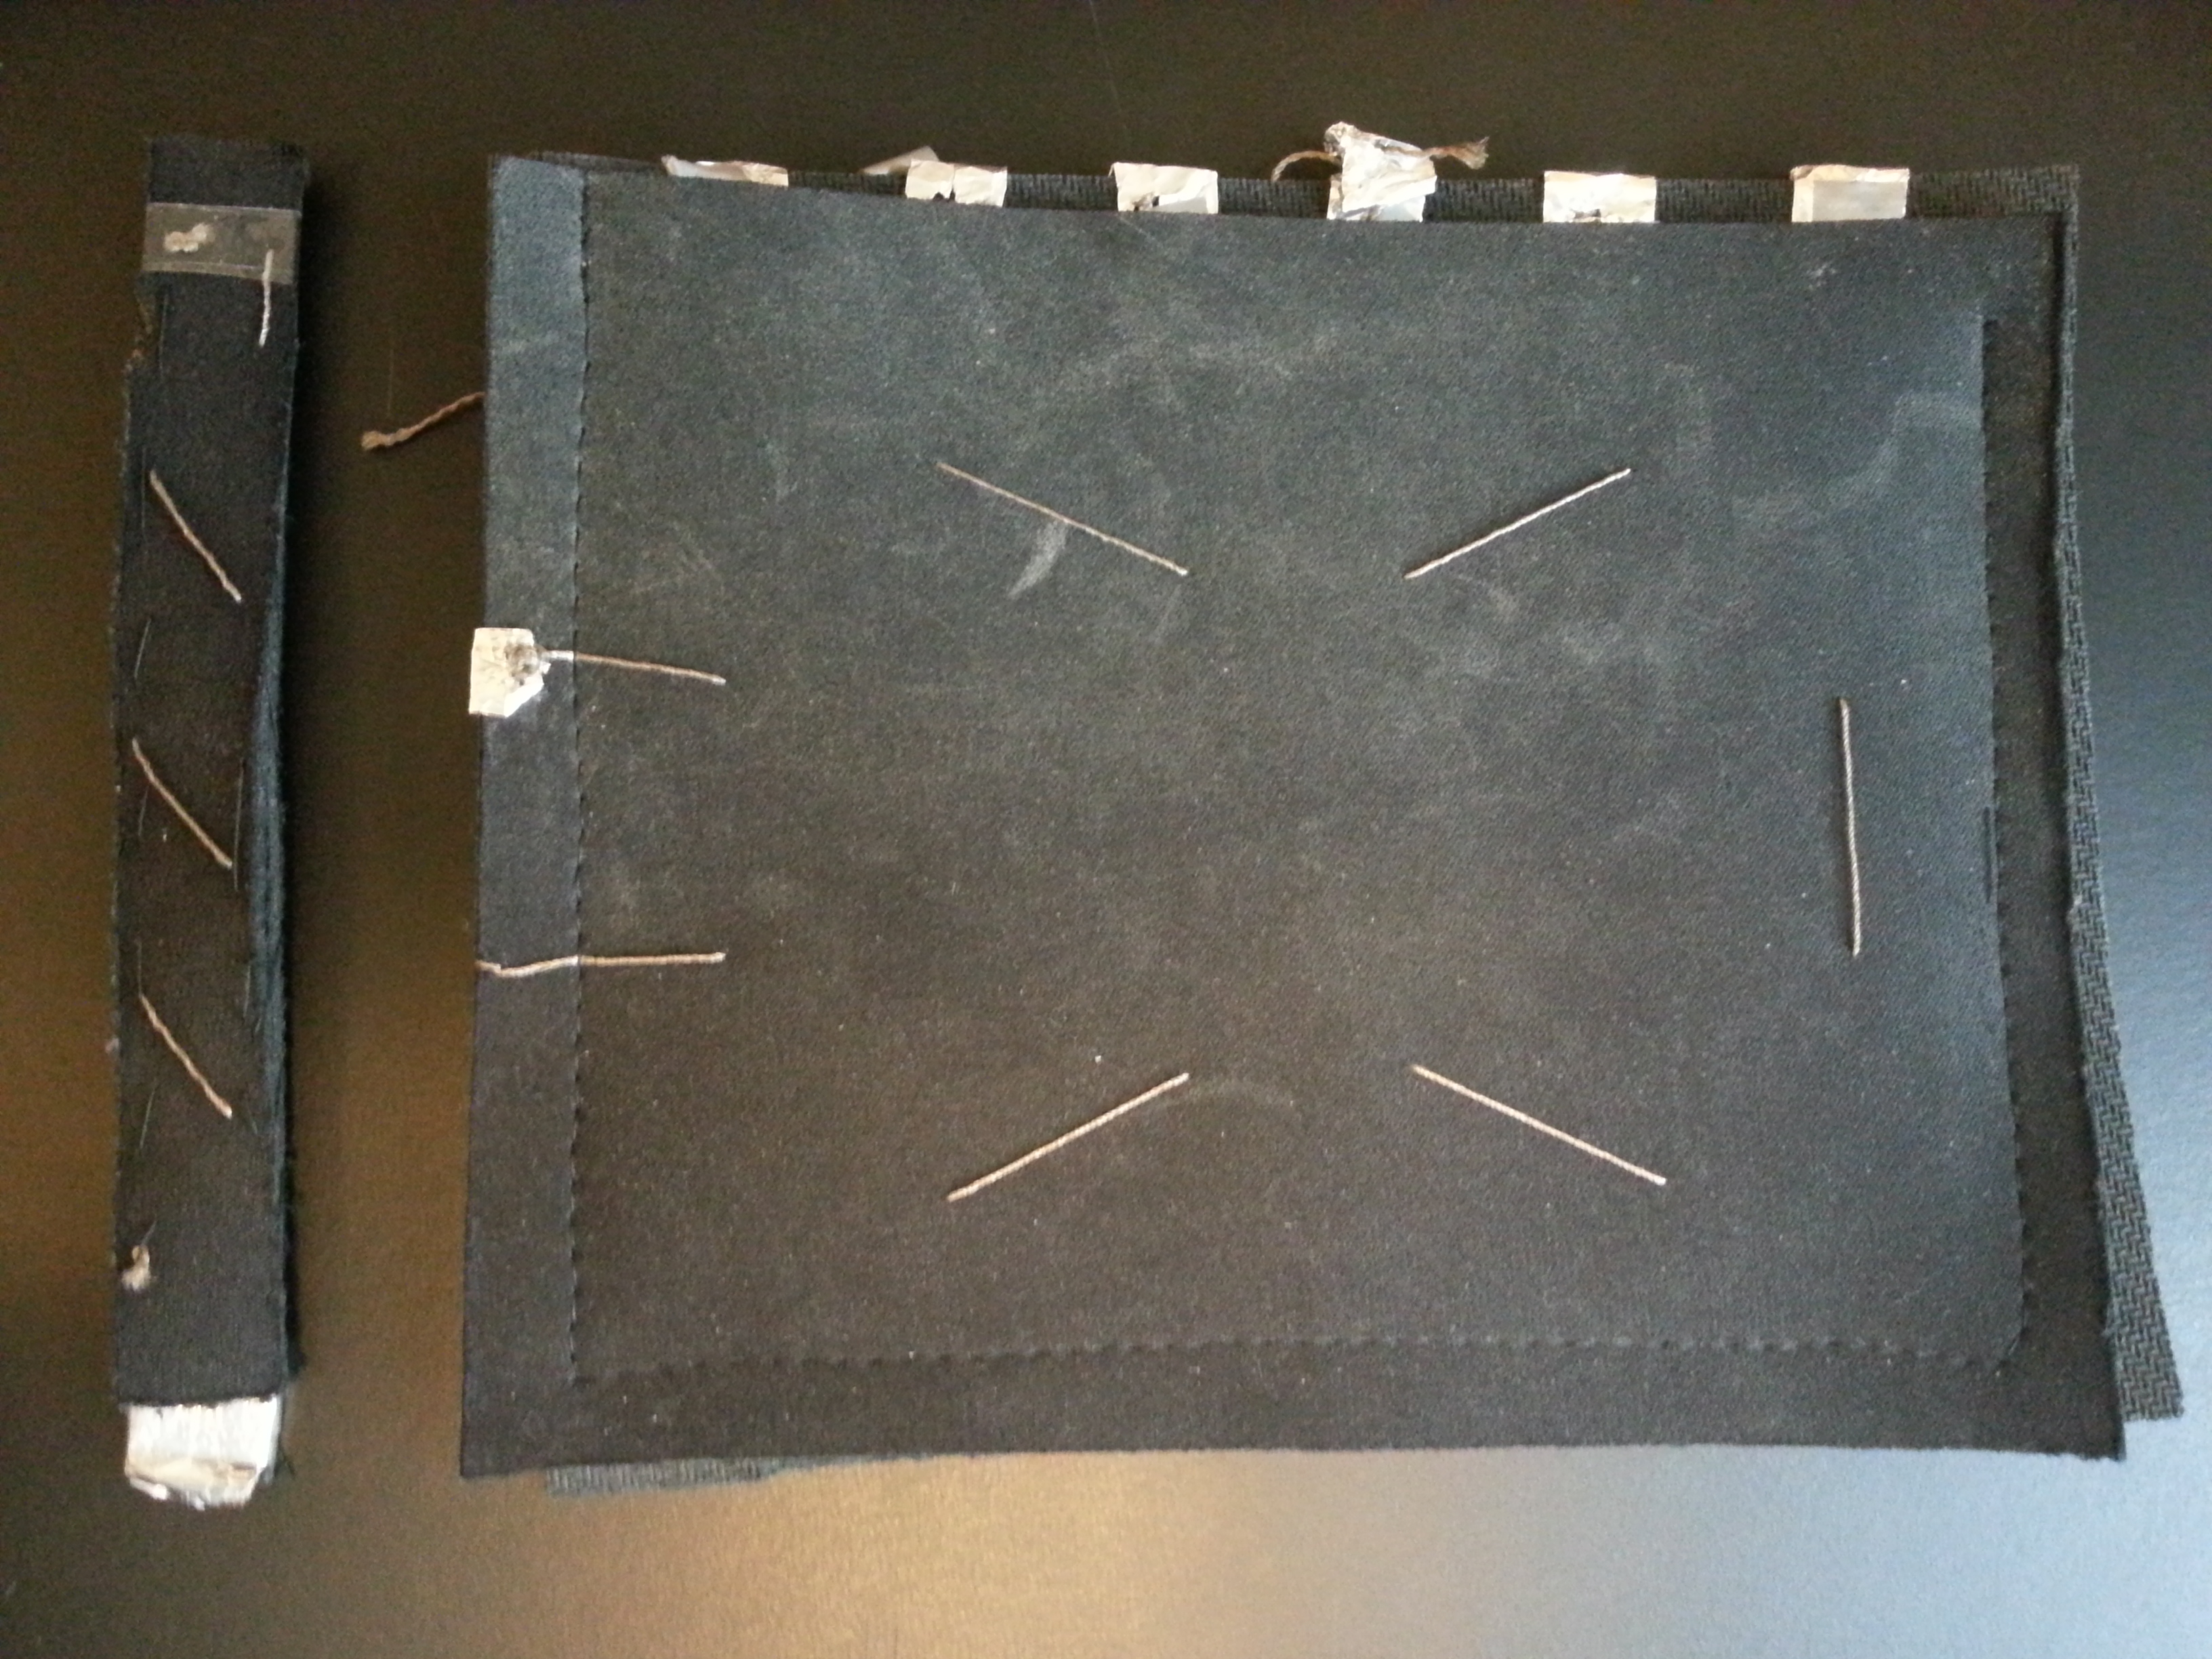
\includegraphics[width=.9\linewidth]{figures/touch/proto1_1}
  \caption{On the left is our simple bend sensor and on the right our 2x3 pressure matrix.}
\end{subfigure}%
\begin{subfigure}[t]{.5\textwidth}
  \centering
  \includegraphics[width=.9\linewidth]{figures/touch/proto1_2}
  \caption{A close up of the materials.}
\end{subfigure}
\caption{First iteration of our touch prototype}
\label{prototype_1}
\end{figure}

By sending a 5V signal into the single top layer stitch, each of the six (\(2*3\)) bottom layer outputs can now be read on the Arduino after passing through the piezoresistive material.  
As pressure is applied to the different sections the voltage drop at the individual grid locations can now be measured with the analog input pins on the Arduino.
The ADC on the Arduino then translates the measured voltage, between 0--5V, into the amount of pressure that is applied to each of the cells, as a number between 0--1023.
The measured numbers will never reach the extremes as there is always some amount of resistance in the material.
A single layer of our anti-static bags have resistance values from around 180-200 KOhms, with little to no pressure applied, down to around 1.8 kOhms when pressed hard.
Depending on the piezoresistive material and the construction of the sensor, these values will vary, \citep{rosenberg2009unmousepad} reports values between 1.2 MOhms and 2.2 kOhms for their FSR ink.

\begin{figure}[h]
	\centering
  		\includegraphics[width=3in]{figures/touch/layers_it_1}
	\caption[The three layers of our touch sensitive fabric, iteration 1.]
   {The three layers of our touch sensitive fabric showing the construction principle of iteration 1.}
   \label{layers_iteration1}
\end{figure}

Each of the cells acts in principle as a discrete sensor as they have their own individual output and are not influenced by each other.
This approach is simple, both in terms of Arduino setup and coding, and can attain the fastest possible update rates as no computation is needed to determine the location of the touch. 
The data received from the sensors is sent to Processing for visualization as can be seen in figure~\todo{ref} which we have used for testing.

\subsubsection{Conclusion}
This quite simple prototype showed us that the basic principles for constructing a textile touch surface with the materials we have had access to, is indeed possible.
One of the major obstacles we found though was the transition from soft electronics (thread and anti-static bags) to hard electronics, as the conductive metal in the threads are woven into normal cotton thread, making soldering extremely hard.
For this first iteration we made due with glued on tin foil connectors as a quick-and-dirty solution.

A major downsides to making touch surfaces as a grid of discrete sensors, as we did in this iteration, is the lack scalability.
There has to be an input pin for each cell in the touch grid you create, so for a given number of rows \(i\) and columns \(j\) you need hardware I/O pins equal to \(i*j\), which is not a suitable for normal micro-controllers which usually have 10--20 I/O pins.
So with this approach we would, just barely, be able to make a 4 x 4 grid with our Arduino Uno. 

\subsection{Iteration 2}
\label{ch:textiletouch:it2}
To combat the lack of scalability in iteration 1 we build a new version of the prototype.
To increase our touch surface resolution we improved the prototype in two ways, first by an improved construction and sewing approach inspired by rSkin \citep{rSsininstructables,rskinplusea} and secondly with interpolating post-processing of the input data inspired by \citep{rosenberg2009unmousepad}. 

\subsubsection{Construction principles}
For the second iteration we made a new 7 x 7 grid prototype, as seen in figure~\ref{prototype_2}, and instead of neoprene, we used sofa textile to get a more natural look and feel, and a larger degree of flexibility in the material.
We used the same basic three layer principle from iteration 1, but in order to solve the scalability issue the conductive thread is sewn in rows and columns as illustrated in figure~\ref{layers_iteration2_and_3}.
The principle is to first activate row 0, then read the output on each of the columns, then activate row 1 and read output on all columns, and so on, contentiously scanning the grid one row/column at a time.
To reduce the sensor noise non active rows and columns are connected to ground throughout the sweep.
Each finished sweep outputs a pressure map that is sent to our applications.

\begin{figure}[h]
	\centering
  		\includegraphics[width=3in]{figures/touch/layers_it_23}
	\caption[The three layers of our touch sensitive fabric, iteration 2 and 3.]
   {The three layers of our touch sensitive fabric showing the construction principle of iteration 2 and 3.}
   \label{layers_iteration2_and_3}
\end{figure}

As only one row and one column are active at a given time the micro-controller now only needs to have one I/O pin for input and one for output and can instead rely on multiplexers\footnote{http://en.wikipedia.org/wiki/Multiplexer} to shift the currently active row/column.
As a result the number of I/O pins now needed is dependent on the number of multiplexers that are used, greatly reducing the number needed for larger grids.

Generally for a multiplexer with \(2^n\) inputs, n control pins are needed plus one pin for the actual signal.
So for a \emph{j} x \emph{i} grid, the amount of pins needed would be \(\sqrt{j*i}\), compared to the \(i*j\) from iteration 1, reducing the amount of I/Os needed by the square root.

As mentioned earlier, if pressure is applied to the piezoresistive material the resistance decreases.
So if the fabric is bend or deformed in any way, this will happen, as the deformation puts stress on the material.
To allow the fabric to be bendable while attaining sensitivity we added a function to `reset' the pressure map by taking a snapshot of the pressure map in its bended state and use this snapshot to subtract from the outputted pressure map.

\begin{figure}[h]
\centering
\begin{subfigure}[t]{.5\textwidth}
  \centering
  \includegraphics[width=.9\linewidth]{figures/touch/proto2_1}
\end{subfigure}%
\begin{subfigure}[t]{.5\textwidth}
  \centering
  \includegraphics[width=.9\linewidth]{figures/touch/proto2_2}
\end{subfigure}
\caption{Second iteration of the prototype. The interactive area is a 7 x 7 grid with each row and column spaced approximately 1 cm apart from each other.}
\label{prototype_2}
\end{figure}

We now have a 7 x 7 grid fabric pad which in it self gives us a resolution of 49 cells compared to the 6 from iteration 1.
To increase this even further we now go from hardware to software.

\subsubsection{Peak detection and interpolating FSR}
\label{ch:textiletouch:it2-ifsr}
If a touch is made between two rows or columns or current approach will register the touch at the closest row/column intersection instead of the true position.
To improve on this aspect, \citet{rosenberg2009unmousepad} presents a new approach to making FRS sensors called IFSR, or Interpolating Force Sensitive Resistance, in their UnMousePad project. The basic principle is to utilize that each sensor cell has overlapping regions of sensitivity with its neighbours.
This overlapping sensitivity is due to the fact that pressure at some position would also affect the surrounding neighbours as they are connected though the resistive middle layer.
This causes a spatial drop-off in sensitivity at the surrounding neighbours that is near linear for both the X and Y axis.
The fact that it is linear on both axes allows for bilinear interpolation to determine the location of touches between the conductive row/column lines, effectively increasing the resolution. 

Compared to the UnMousePad, which uses printed conductors, our fabric approach is a lot less `perfect' in its construction precision.
At the same time the fabric can bend and twist a lot more that a sheet of polymer, all in all generating a less precise pressure map which translates into less precise interpolation.
As a result we have taken a slightly more simple approach to the interpolation than \citep{rosenberg2009unmousepad} and in turn sacrificed some of the possible resolution gain.
\blank
For a given touch we first find the max value of the nearest intersection of the touch, point \(P_{max}\).
Because a touch gives a radial spread of current around itself, the precise location of the touch will always be in the region of the \(P_{max}\).
As there is a linear drop-off we can now take the readings from the surrounding \((X_{max}\pm1,Y_{max}\pm1))\) and use them them to do a weighted average on both axes to approximate the correct position.
The new approximated point \(P_{approx}\) will, as a result of the radial spread, have a higher weight than the sensed \(P_{max}\) so we scale the value of \(P_{approx}\) with a factor according to the euclidean distance to \(P_{max}\). 

\todo{maaske lidt mere her}

\todo{lav en af ligning interpolationen?}

\begin{figure}[h]
\centering
\begin{subfigure}[t]{.45\textwidth}
  \centering
  \includegraphics[width=.9\linewidth]{figures/touch/p_map}
  \caption{Visualization of the raw touch data, black indicate no pressure and white indicate high pressure.}
\end{subfigure}%
\hspace{0.5cm}
\begin{subfigure}[t]{.45\textwidth}
  \centering
  \includegraphics[width=.9\linewidth]{figures/touch/p_approximation}
  \caption{The weight-approximated position, based on the raw touch data from (a). The blue circles indicates the intensity of the values of the sensor cells surrounding the \(P_{max}\).}
\end{subfigure}
\caption{Illustration of the interpolation process.}
\label{interpolation}
\end{figure}

\subsubsection{Conclusion}
For this type of application where a large number of individual sensor cells are needed the construction approach we have used in this iteration is by far superior to the one from iteration 1.
It is a more complex setup both in software and hardware but it does in turn enable much larger sensor arrays than before as we showed before with the amount of I/O pins needed.
As it scales up it is of course more computational heavy on the Arduino CPU as the multiplexers and, in our case, 49 sensor cells needs to be controlled, but as this is still only a 7 x 7 grid we did not experience performance problems.

The interpolation point approximation was, to some degree, a success as it enabled us to up-scale the resolution with a factor 5 with only few approximation errors, but when scaled with a factor 10, which was the goal, quite a few errors appeared.
Many of these errors are due to the sewing of the conductive thread as it, because of the close seams, protrudes a bit where the stitches are, which can be seen by looking at figure~\ref{prototype_2}.
Also the fact that the precision of the sewing are not machine-accurate somewhat eliminates the linearity that we base our interpolation on, creating errors in the raw data that are hard to even out in the software.

\subsection{Iteration 3}
\label{ch:textiletouch:it3}
One of the focus areas of iteration 3 was build a larger and more precise version of iteration 2 as to get more reliable raw data from the sensor grid to use for gesture interaction.
As we were aware of the possibility of generating imprecise data, as we have discussed in the previous iterations, from physical deformation, construction imprecision, material variations and approximation errors, the second focus was to implement a basis for gesture recognition that would function under these constraints.

\subsubsection{Construction Principles}
We used the same setup of iteration 3 but scaled to a 16 x 16 grid, providing 256 sensor cells after software upscaling, compared to the 49 of iteration 1.
The prototype was made in linen which is robust but a lot finer and thinner that the sofa textile and the conductive thread was sewed with less close seams to avoid some of the problems from iteration 2.
The prototype can be seen in figure~\todo{ref} and the schematics for the final hardware setup can be seen in appendix \ref{app:textile-touch}.

One of the main challenges in the construction of this iteration was the attachment of the wires to the conductive thread.
In iteration 1 we tried with glued on tin foil which only worked because we only had 6 connections to handle.
The 14 connections in iteration 2 were connected with alligator clips which, besides not looking elegant, tend to cause deformation of the fabric as they close upon it.
As we now had 32 connections to deal with we found that using ribbon cables would give a better structure.
Furthermore, as alligator clips were out of the question and as tin and textile do not work well together we needed to find an alternative for the connection.
Conductive paint turned out to be a good substitute and worked as a kind ``cold''-soldering method - a secondary feature of the paint.
As the paint dries it functions like an adhesive but with the added ability of being conductive so you avoid the risk of the glue get in between the two conductors severing the connection, see figure~\ref{fig:ch:textiletouch:barepaint}.

\begin{figure}[t]
\centering
\begin{subfigure}[t]{.45\textwidth}
  \centering
  \includegraphics[width=.9\linewidth]{figures/touch/barepaint}
  \caption{Bare Paint, an electrically conductive ink, found at www.bareconductive.com}
\end{subfigure}%
\hspace{0.5cm}
\begin{subfigure}[t]{.45\textwidth}
  \centering
  \includegraphics[width=.9\linewidth]{figures/touch/connectors}
  \caption{Bare Paint, used for ``cold''-soldering wires to conductive thread.}
\end{subfigure}
\caption{One solution for the challenge of connecting conductive thread to wires.}
\label{fig:ch:textiletouch:barepaint}
\end{figure}

\subsubsection{Data flow}
In figure~\ref{fig:textiletouch:dataflow} we illustrate each major step in the data flow and processing 
of our prototype.
The flow of data starts from sensor data in the \emph{physical layer} read by the Arduino.
Thereafter it is converted to digital data and streamed to the \emph{processing layer}.
In the \emph{processing layer} the data goes through several filter stages to optimise the data.
Lastly the filtered data is delivered to \emph{application layer} where data can be translated into gestures or visualisations.
We have already covered the principles of the physical layer in \ref{ch:textiletouch:it1} and peak detection and interpolation in \ref{ch:textiletouch:it2}.
Next we will cover some additional steps in the data flow and the \emph{application layer}.

\begin{figure}[b]
  \centering
      \includegraphics[width=\textwidth]{figures/touch/dataflow}
  \caption[The data flow from sensor to application.]
   {Textile Touch data flow from sensor to application.}
   \label{fig:textiletouch:dataflow}
\end{figure}

\subsubsection{Noise reduction}
On the software side we have implemented a simple averaging filter to reduce noise by increasing the signal-to-noise ratio, SNR.
This filter takes each input frame and averages the values of each cell with the cell values of \(x\) previous frames.
We have found that averaging over the past \(x = 2\) frames gives the best result for our setup. 
\todo{udpensles mere?} 
In this way noise such as sudden spikes will be reduced while preserving the actual touch values of the frame.

\subsubsection{Peak detection and interpolation}
The algorithm for detecting touch input and interpolation has generally not changed since iteration 2, see~\nameref{ch:textiletouch:it2-ifsr} in \ref{ch:textiletouch:it2-ifsr}.

The new part is that we in iteration 3 also have introduced multi-touch input.
This is more a proof of concept feature which will not be fully functional and stable for interaction. The reason for this is that our code needs some adjustments to be able to provide proper stroke data to the recognition framework which would require too much implementation time.
So for now we can visualise multi-touch input and basically use it for drawing, see figure~\ref{fig:textiletouch:multitouch}.

An alternative would be to serve all recorded touch points to the \$N implementation, as opposed to \$P, \todo{but as noted earlier} this would be unsatisfactory slow.

\begin{figure}[h]
  \centering
      \includegraphics[width=.9\textwidth]{figures/touch/tt_multitouch}
  \caption[The data flow from sensor to application.]
   {Multi-touch input visualised. 3 fingers are detected and 3 lines are drawn simultaneously.}
   \label{fig:textiletouch:multitouch}
\end{figure}

\subsubsection{Gesture recognition} 
\label{ch:textiletouch:gesture_implementation}

We have created an application that takes the filtered data of the \emph{processing layer} and abstracts it to a collection of strokes that are delivered to the \$P gesture recognition framework, which matches the input up against a set of predefined gestures templates.
The dollar family of recognizers were presented earlier in \ref{ch:textiletouch:gesture_recognition}.
Initially we experimented with the \$N implementation which was able to recognise gestures but with some limitations.

First of all, the recogniser was sensitive to the ordering of the strokes which meant that the it could fail on the same gesture if drawn from different starting points. \todo{Tore, yes?}

Secondly, there was a considerable amount of delay before a resulting gesture was found.
We measured this to be in the area of \(800\) to \(1000 ms\), a latency which in our opinion does influence the user experience.
After changing to the \$P implementation we got this delay down to \(< 10 ms\) which is quite an improvement.
This is because \$P avoids a combinatorial overhead of \$N where \$N matches up against every possible combination of stroke order and direction.

Furthermore, the \$P implementation does not distinguish the order of the strokes which allows for subjective ways of drawing specific shapes.

One limitation of both implementations is that they do not take in to account the orientation of the input. 
This means that, for example, for a line to be recognised in both a vertical, horizontal and diagonal version they all need to have a predefined template. \todo{say something about the complexity of writing templates? P vs N}

\subsubsection{Feedback} 

\subsubsection{Conclusion} 

Although the 3rd iteration overcame some of the limitations of the 2nd iteration it still has some constraints that we would like to address.

One noticeable limitation is performance as foreseen in interation 2.
Our current Ardiuno Uno is not fast enough to always follow along with quick touch movements on the prototype.
Simple gestures like lines or simple characters are not affected as much as more complicated symbols.
The new and exceedingly faster Arduino Due\footnote{http://arduino.cc/en/Main/ArduinoBoardDue}, an ARM-based board which operates at a clock speed of 84 MHz, has recently been released and would greatly outperform our older 8 MHz Arduino Uno.

One of the reasons for scaling up the prototype was to get a larger area for touch input.
In the process of tripling the dimensions of the prototype (from approximately \(8x8cm\) to \(25x25cm\)) we also increased the amount of rows and columns but with a little extra spacing (\(1.5cm\)) between the individual lines.
It seems that this spacing has become a bit too large, meaning that pressing in between the intersections of two rows and two columns does not propagate quite enough pressure to the surrounding line crossings, resulting in smaller pressure values (see figure~\ref{fig:textiletouch:intersections}).

We have tried to improve this in our approximation algorithm by multiplying the value with a factor relative to distance away from the line in both axes.
This has to some degree amended the issue but not fully.

\begin{figure}
\centering
\begin{minipage}[t]{.45\textwidth}
  \centering
  \includegraphics[width=.9\linewidth]{figures/touch/intersections}
  \caption[Pressing in between the intersection of two rows and two columns does not propagate enough pressure.]
  {Pressing in between the intersections of two rows and two columns (red dot) does not propagate enough pressure to the surrounding lines crossings (blue dots).}
  \label{fig:textiletouch:intersections}
\end{minipage}%
\hspace{1cm}
\begin{minipage}[t]{.45\textwidth}
  \centering
  \includegraphics[width=.9\linewidth]{figures/touch/wires}
  \caption[Breadboard crowded with wires.]
  {Breadboard crowded with wires.}
  \label{fig:textiletouch:wires}
\end{minipage}
\end{figure}

An alternative approach is to reduce the spacing again to \(1cm\) or less but that would require quite a few extra wires which we already have quite a few of (see figure~\ref{fig:textiletouch:wires}).
Furthermore increasing the grid resolution would result in an exponential growth in the amount of data to be transmitted by the microcontroller.
With a \(16x16\) grid we are sending 256 values every frame (\(10ms\)),
If we were to lower the spacing to \(1cm\) we would get a grid resolution of \(24x24\) which in turn would require a transmission of 576 values for every frame.
As our microcontroller is already running at over capacity this out of the question for now, but by replacing the microcontroller with a more powerful one, as mentioned before, increasing the resolution could become relevant again.
Therefore we see it as a balance between the size of the touch area and the complexity of the hardware setup.

\begin{verbatim}
- Fokus paa kode (gestures,resolution,performance)
- Interpolering muliggoere tryk mellem linjerne, 10x saa hoej oploesning dog udfald 
  og varierende praesision (vis vi har eksperimenteret med forskellige oploesninger)
- Forskellige visualiseringer til performance evaluering
- Integrering af gesture recognition og test miljoe til dette
- Haptisk feedback, vibration
- Udfordringer: praesision, performance 
  (max baud-rate for hurtigt til at java kunne foelge med)
\end{verbatim}

\section{Evaluation and future work}
%!TEX root = ../thesis.tex
In this section we are going to cover our evaluation of our \emph{textile touch} explorative prototype, more specifically this is the latest prototype covered in \ref{ch:textiletouch:it3}~(\nameref{ch:textiletouch:it3}).
We have two primary goals of this evaluation.
On the one hand, we want to evaluate on the interaction potentials of using simple gestures as input control.
This goal involves using the prototype as an interactive device to control existing devices of the home.
On the other hand, we want to explore our prototype in alternative contexts.
This goal should shed light on the prototypes potential of encouraging alternative usages than controlling existing devices.

Evaluations were done over three rounds to get a diversity in age groups of the test participants and also to evaluate both technical and non-technical people.
\hl{We were interested in shedding light on the diversity of creative ideas a child would bring compared to and adult.
}
\todo{mere + afrunding}
\blank
As mentioned earlier in \emph{ \nameref{ch:textiletouch:it3} } we have developed a simple audio and video application which mimics some of the functionality of a television and a stereo system.
This application was used as the starting point for evaluating the value of using the prototype for controlling existing devices.
During evaluation we would connect the prototype setup and computer to the home TV to resemble the real situation and the prototype would for instance be layn as part a of sofa, as a table cloth or attached to a wall as for example wallpaper.
From there on the basics of interaction were understood and further discussions and explorations could be made extending beyond the limits of the audio/video application.

Moving on from looking at the potentials of controlling existing devices of the home, the evaluations would take a more discussion-oriented direction where alternative usages and activities were the primary focus.
To start off discussions we would present some of our own ideas of potential usages.
\todo{mere}
\blank
An overall note to be taken from the evaluations was that the participants found it intriguing to try out the prototype.
Not so much for the purpose of the simple test application, but more for the idea of interacting with textile and using it for digital input.
Surely they are accustomed to using touch interaction on the small surfaces of everyday consumer devices such as displays and touchpads, but not with inherently non-electronic materials such as textile. \todo{lidt mere generelt her}
\blank
In the next section we will evaluate on the performance of our prototype and then continue on with the conceptual potentials in the subsequent two sections.

\subsection{Performance and feedback}

In this section we will discuss the prototype concerning performance and feedback and some of the improvements suggested during evaluations.

% refresh rate
The limitations of the refresh rate of the hardware were noticed by all participants.
The consequence was that they had to perform touch input in a more careful manner and with slower motions than they wanted to.
The participants' touch strokes were in general much faster than anticipated, which is likely due to us having done much of our testing during development and therefore have been more careful.
They were all able to adapt to it and perform their intended actions with success, but it did of course put a constraint on the interaction.

% softness
In our first evaluation we tested a scenario with a sofa with textile touch embedded.
The softness of the sofa made touch input readings inconsistent and unstable.
The reason for this was that the prototype was not part of the sofa construction which makes even small movements and pressure inputs push the prototype around on the surface of the sofa.
This makes the pattern that constitutes a touch look different than when used on a hard surface which we have not taken into account in our software.

% fb: vibrations
The idea of a pulsating vibration during touch was well received as an indication of touch being recorded and to delimit for example the digital sofa from the physical sofa. \todo{what?}
As we anticipated, the haptic feedback got some critique and it was pointed out that it should give a stronger sensation.
We had placed the vibration motor in the center beneath the prototype and vibrations were therefore only noticeable in that area.
With a less powerful motor the subtle touch sensation of ones hand against the texture of the linen could easily drown the vibrations as well.

% fb: visual on display
A concern brought up by several participants was that there was a lack of indication of the stroke one had just applied.
A promising visual feedback technique for display-oriented interaction was suggested by one of the participants.
The idea was to get real-time feedback on a display when providing touch input by seeing the strokes being made as an overlay on the display.
The strokes would then quickly fade away again to not obstruct the viewing experience. 
In figure~\ref{fig:textiletouch:eval:overlay} we have made an illustration of two semi-transparent strokes overlaying a TV programme as example. 

% fb: visual through LEDS
This visual feedback technique could be very convenient when actions are directed towards a device with a digital display, but not possible in a display-less context.
The single LED we installed beneath the prototype did not prove to be very useful by itself, but its ability to shine through the linen did show potential.
We discussed a larger deployment where a low resolution grid of tiny LEDs could be embedded beneath the textile surface and follow movements by illuminating at touch points and get a direct visual feedback, see figure~\ref{fig:textiletouch:eval:backlighting}.
This approach is again limited to applications where the surface material allows for illumination to shine through, but it does extend beyond textile materials.

\subsection{The concept as a controller for existing devices}
\todo{\dots}
\blank
\begin{verbatim}
taler til det indre dovendyr (paw)
   rette paa gardiner
skal i hvert fald ikke blive et komplekst nyt sprog man skal laere
   ensartet interaktion paa tvaers af applikationer
teenager forstod med det samme - mega smart ;-)
  fandt det let at interagere med
"fjernbetjening er en forlaengelse af min arm" (paw) - dette er dog et lidt vagt modargument
\end{verbatim}

\begin{figure}[h]
  \centering
  \begin{subfigure}[t]{.44\textwidth}
    \centering
    \includegraphics[width=\linewidth]{figures/touch/evaluation/gesture_overlay}
    \caption{The real-time overlay during touch. This ascending or descending two stroke gesture could for instance mean 'volume up' or 'down'.}
  \end{subfigure}%
  \hspace{0.02\textwidth}
  \begin{subfigure}[t]{.44\textwidth}
    \centering
    \includegraphics[width=\linewidth]{figures/touch/evaluation/gesture_overlay_2}
    \caption{The indication that a 'volume' action was performed.}
  \end{subfigure}
  \caption{Gesture input as an overlay for real-time feedback.}
  \label{fig:textiletouch:eval:overlay}
\end{figure}

\begin{figure}[h]
  \centering
  \begin{minipage}[b]{.8\textwidth}
    \centering
    \includegraphics[width=.7\linewidth]{figures/touch/evaluation/backlid_textile}
  \caption[Illumination directly beneath touch points.]
  {Illumination directly beneath touch points.}
  \label{fig:textiletouch:eval:backlighting}
  \end{minipage}
\end{figure}

\begin{figure}
        \centering
        \begin{subfigure}[b]{0.44\textwidth}
                \centering
                \includegraphics[width=\textwidth]{figures/touch/evaluation/sebastian/in_sofa}
                \caption{\dots}
                \label{fig:textiletouch:eval:sebastian:sofa}
        \end{subfigure}%
        \hspace{0.02\textwidth}
        \begin{subfigure}[b]{0.44\textwidth}
                \centering
                \includegraphics[width=\textwidth]{figures/touch/evaluation/sebastian/sofa_behind_seb}
                \caption{\dots}
                \label{fig:textiletouch:eval:sebastian:sofa_behind}
        \end{subfigure}

        \begin{subfigure}[b]{0.44\textwidth}
                \centering
                \includegraphics[width=\textwidth]{figures/touch/evaluation/sebastian/sofa_infront_seb}
                \caption{\dots}
                \label{fig:textiletouch:eval:sebastian:sofa_front}
        \end{subfigure}%
        \hspace{0.02\textwidth}
        \begin{subfigure}[b]{0.44\textwidth}
                \centering
                \includegraphics[width=\textwidth]{figures/touch/evaluation/sebastian/table}
                \caption{\dots}
                \label{fig:textiletouch:eval:sebastian:table}
        \end{subfigure}
        \caption{Teenager during evaluation \dots}
        \label{fig:textiletouch:eval:sebastian}
\end{figure}

\begin{figure}[h]
  \centering
  \begin{minipage}[b]{.8\textwidth}
    \centering
    \includegraphics[width=.7\linewidth]{figures/touch/evaluation/sebastian/feet}
  \caption[Feet \dots]
  {Feet \dots}
  \label{fig:textiletouch:eval:sebastian:feet}
  \end{minipage}
\end{figure}

\begin{figure}
        \centering
        \begin{subfigure}[b]{0.44\textwidth}
                \centering
                \includegraphics[width=\textwidth]{figures/touch/evaluation/kaia-gitte-troels/alle}
                \caption{\dots}
                \label{fig:textiletouch:eval:kaia-gitte-troels:alle}
        \end{subfigure}%
        \hspace{0.02\textwidth}
        \begin{subfigure}[b]{0.44\textwidth}
                \centering
                \includegraphics[width=\textwidth]{figures/touch/evaluation/kaia-gitte-troels/kaia-gitte2}
                \caption{\dots}
                \label{fig:textiletouch:eval:kaia-gitte-troels:kaia-gitte2}
        \end{subfigure}

        \begin{subfigure}[b]{0.9\textwidth}
                \centering
                \includegraphics[width=\textwidth]{figures/touch/evaluation/kaia-gitte-troels/kaia-gitte}
                \caption{\dots}
                \label{fig:textiletouch:eval:kaia-gitte-troels:kaia-gitte}
        \end{subfigure}
        \caption{Teenager during evaluation \dots}
        \label{fig:textiletouch:eval:kaia-gitte-troels}
\end{figure}

\subsection{Potentials of alternative usages}

The ideas for alternative usages were in general very different from the idea of controlling existing devices.
The ideas were more characterised by sensor data being used in situations where meaning is open to interpretation as opposed to a one-to-one mapping between input gesture and function.
For example, several ideas concerning safety and security were discussed.

% toddlers
Parents of toddlers often have floor mats for their child to lay and play on, see figure~\ref{fig:textiletouch:eval:softtiles}.
Instead of having parents checking up on their child every two minutes these mats could have touch fields embedded.
The sensor data can then be abstracted to inform parents about the activity of their child by recording pressure and movement, giving the concerned parent room to do less frequent check ups.
This is actually a very simple setup that does not require a high resolution of the sensor grid and the output required could be condensed to simple states such as, whether the toddler is on the mat and the level of movement activity.

% elders
Elderly people with a weak physic or people with Parkinson's disease have a tendency to fall over easily.
One of the approaches in reducing the consequences of a fall is to give the elders assistive devices such as wearable fall detectors which can automatically release an alarm in the event of a fall.
An alternative approach, which does not require body equipment, could be to prepare the home with sensitive impact sensitive floors or carpets.
Some may base their sense of security in a physical wearable device while others find it inconvenient, a source of irritation, or maybe even an exceedance of personal privacy. 
With safety measurements invisibly integrated into the home the sense of security may be directed towards to the scope of the home as a whole.

% handicap
Some disabled people with hindered mobility 
\blank
% Home security
During the evaluations we also discussed a scenario of home security regarding the front door of ones home.
In this scenario we imagined a blank door with no handle and no lock and thereby no need for a key.
Instead the door had an embedded grid of pressure sensors.
We came up with and enacted two different interaction styles for opening the door.
One was a variant of the pattern lock found in many Android smart phones where a set of points must be touched in the correct sequence in order for the door to unlock, see figure \todo{billede af Kaia og Gitte ved doeren 1}.
The other was based on the fact that people have unique signatures which could be used for authentication.
A person would then have to makes strokes (the signature) on the door facade to be authenticated and have the door unlock and open, see figure \todo{billede af Kaia og Gitte ved doeren 2}.

This is a good example of an ad hoc interface \emph{through invisible interfaces embedded into the physical environment}.
Knowledge of the system is a prerequisite to enter in that you are faced with a blank facade with no direct indication of how to enter.
It also confronts the raised issue of invisible interfaces and affordances by using it as an advantage in a security setting where the absence of a lock and door handle would inhibit a trespasser.
\blank
% Sleep cycle
Moving away from the topic of safety and security and to the topic of self-tracking, a movement that has gained a lot popularity in recent years with the advent of consumer gadgets, such as Fitbit\footnote{http://www.fitbit.com/}, Nike+\footnote{http://nikeplus.nike.com/plus/} and loads more. 
These gadgets let you sense just about anything concerning your body, quantifying yourself in numbers.
An example of this is sleep monitoring and optimisation, which in its simplest form only requires a smart phone next to your body in bed, but can take on more advanced forms as well with a variety of body sensors.
With a smart phone the approach is to use the built-in accelerometer to detect movement during sleep to graph the total sleep and derive whether the person is in deep sleep or light sleep.
These data can also be used to trigger the wake-up alarm at moments of light sleep within a specified time frame close to the set alarm time.

A product with the capabilities of our textile touch prototype which can infer the same kind information by the means of a pressure measurements over time, would be an interesting alternative.
Being integrated as part of a madras or a bed sheet it would be unnoticeable for a sleeping person and would not require a smart phone next to the pillow which some may be precautious about.

This application does not really fall under the category of AHIs, but it is mentioned here for the potential of a discrete and unobtrusive product as a continuation of the self-tracking movement.


\begin{figure}[h]
  \centering
  \begin{minipage}[b]{.8\textwidth}
    \centering
    \includegraphics[width=.7\linewidth]{figures/touch/evaluation/softtiles}
  \caption[Toddler on a foam floor mat with puzzle-like tiles for extensibility.]
  {Toddler on a foam floor mat.}
  \label{fig:textiletouch:eval:softtiles}
  \end{minipage}
\end{figure}

\begin{verbatim}
**** Paw + Morten ****
* tegning paa overflader: "hvis danmark nu er her ... og holland her, saa ..." 
	- for at forklare ting.
* boernevaerelse - legemaatte, hvor foraeldre kan se aktivitetsniveau for 
	deres unger og dermed ikke behoever at tjekke op paa dem hele tiden.
* handikaphjem
	* vildt mange ting der skal styres
    * mobilitet er begraenset
* aeldrehjem
    * crash taeppe - folk med parkison der ofte vaelter eller lign.
        * eller alle flader
    * "hvis man ikke har noget paa kan det ikke tages" - nuvaerende situation 
		hvor aeldre faar "halsbaand" (falde-detektor) paa, som de tager af i tide og utide.
* Sikkerhed. Den usynlig noegle - man skal vide hvor man input delen er for 
	at kunne lave en "adgangsgestik".
    * Eller det, at mennesker har en unik "haandskrift" der kan anvendes 
		paa touch overfladen.
    * doermaatte
\end{verbatim}

\subsection{Future work}
\label{ch:textiletouch:futurework}

There are several points about the prototype that are candidates for future work.

% Multitouch
On the technical side there is room for improvement.
As the technology allows for multi-touch input it would be a great improvement for the user experience.
Multi-touch provides a much richer interaction style \todo{reference?} compared to single-touch and has become a standard in modern smart phone displays and laptop touchpads, most notably for scrolling, zooming and rotation.
The gesture recognition framework used for the prototype, \$P, will work just fine with multi-touch and will not require further adjustment as the method of input is totally decoupled from the recognition framework. \todo{though gestures or symbols are not the same as real-time gestures on a mouse-pad such as zooming}
Instead it is our peak detection algorithms that need to be reimplemented and take multiple peaks in to account.
Figure~\todo{ref} shows a frame of input where several peaks made by finger inputs are detected. \todo{provide reason for not implementing multi-touch in the firstplace?}

As can be seen in the figure every peak is surrounded by some noise created by finger pressure propagating away from the peak spot.
It should be noted that we do not consider values in the immediate proximity of a peak to be noise as we use these values to make interpolation and thereby scale the resolution by a factor a 10.
We have already taken steps to reduce this by implementing a simple averaging filter in the software 
where a sample is an average of \emph{x} previous samples.
There are also steps to be taken on the hardware side where a noise filter could reduce the signal-to-noise ratio before entering the software part.

\todo{ting der er belyst fra evaluering \dots}

\begin{verbatim}
dette er ikke faerdig prototype - snakke om forskellige retninger
Real-world implementation - e.g. a whole sofa, wall paper?
\end{verbatim}



\chapter{Exploration: Conductive Paint}
\label{ch:proto3}
%!TEX root = thesis.tex
The third approach to creating AHIs that we presented in chapter~\ref{ch:adhoc} was to construct the interface on the spot.
Of the three approaches this is the one that we have explored the least.

----This approach originated from the idea of interfaces that was ``fashioned from whatever is immediately available''.
--While this may not be quite possible, the idea is engaging and intriguing as an embodiment of a very literal version of AHIs. 
we presented this approach as interfaces that was .. .. .. 
But how do you go about making such a system?

\subsection{Related work}
We have done a few, though a bit cursory, experiments to explore the concept.
The main challenge has been to find materials, or a generic enough platform, that allows you to create objects or environments with interactive capabilities from \emph{whatever is immediately available}. 

There exist various physical ``frameworks'' or assembly kits that incorporates at least some of the aspects that we see in this approach to creating AHIs, in the sense that they provide building blocks or a general platform for creating interactive interfaces, that can be dismantled after use.

Examples of the assembly kit approach can be seen in Topobo \citep{raffle2004topobo} and Block Jam \citep{newton2003block}, where the focus is on the topological assembly of the different components of the system. 
Topobo is a physical 3D modelling system where the individual components have kinetic memory. 
The setup employs a mix of passive and active elements where the active components can record kinetic movement and play it back.
The kinetic outcome will then be based on how the different active and passive components are assembled.

Block Jam is a system that uses an array of physical blocks to create a dynamic and tangible sequencer.
In Block Jam the specific positioning of the individual blocks varies the auditive outcome, so while the blocks in themselves does nothing, the collection of blocks forms up an ad hoc dynamic sequencer.
Common for these two examples is that the individual components in the systems, while being part of a larger collection, are non customizable stand-alone object and that it is the topology of the assembly that defines the interactive capabilities.

A more general purpose approach is seen in physical computing platforms such as Arduino, which is a prototyping platform for electronics and one we have used a lot in our prototype work for this thesis, and LEGO Mindstorms\footnote{http://mindstorms.lego.com/en-us/default.aspx} which is a programmable robotics platform.
Compared to Topobo and Block Jam, much less details are abstracted away on the two platforms and therefore gives an increased focus on digital programmability and on more generic components.
As such a specific component does not have a specific application purpose in mind and the topological placement of components are not defined by the platform -- of course wires, actuators, sensors, gears, wheels, and so on, have to be assembled correctly to function.

\todo{bare conductive eksempler}

\todo{relevans til vores approach}

\subsection{Exploration}
We have explored the use of Bare Conductive, an electric water-based paint, as a material for creating AHIs on the spot.
This electrical paint has some interesting properties as it is easily applied and dries quickly but at the same time, because it is water-based, can be removed with a wet cloth.
This fits well with our idea of an interface that is quick to make and quick to erase.

We see two overall options for using a paint like this.
Firstly as a connector where the paint either acts as a wire between two points or as a switch.
Secondly the paint can work as a variable resistor as the paint itself is resistive inversely proportional to the cross sectional area\footnote{Bare Conductive technical data sheet - http://www.bareconductive.com/file/2013-technicaldatasheet-bareconductivepaint-pdf}. 
This means that a thin line will have a higher resistance than a wide line of the same length. 

Inspired by Brand's earlier mentioned six S's \citep{brand1995buildings} we have envisioned a concept where we, instead of hiding it, try to expose the infrastructures of the house.
It is the norm to hide as much of the ``working guts'' of a building from sight.
Electrical wiring and plumbing are embedded into the building itself hindering easy change or modification to these systems.
Our idea is to bring down these services to the layer of Stuff where continuous changes and adaptations can be made as needed.
At the same time it is a move against the tendency of always hiding away the complexity of things behind polished surfaces, instead showing off the complexity as an aesthetic intellectual quality, combining the raw functionality of the service with the expressiveness of paints.

We have taken an offset in the wiring of the house and envision a concept where the wires and switches in the house can be painted on the walls with both the traditional functionality of wires, but also the added ability to create visual interactive expressions.
As the shape of the paint will affect the resistance, as mentioned earlier, this will provide the ability to, at least in some fashion, have the visual expression correlate with the interactive capabilities, combining aesthetic expression with functionality.

We have made a simple video prototype showing the possibility of creating a dynamic light switch on the wall and removing it again.
In figure \todo{ref} a room is shown with its wiring exposed to the inhabitants as a mix of functionality and wall art that can be remade or adapted as they see fit.

So can a paint like Bare Conductive provide ad hoc capabilities?

\subsection{Discussion}
When we started out our exploration of paint as a medium for AHIs we thought that it would be easy to conceptualize and show off some compelling and interesting examples of how this could be used.
We wanted to focus less on the supporting infrastructure and more on the possibilities of using paint, more or less exclusively, as the interface and as the defining property for how the interaction worked. 
However we quickly became severely limited by the fact that our material only supports conduction and resistance and therefore many of the usually given components in physical computing, such as transistors, gates, diodes etc., is not possible to make on the spot, without supporting infrastructure.  

\todo{interesting stuff goes here}

We still feel that the idea of creating the actual material interface on the spot, where the interface is fashioned to your current needs and shaped to your liking by yourself, is wildly enticing, though it might not be entirely realistic.
There is a beauty in the idea of an interface constructed from a simple material, that can be washed away when it is no longer needed, but still provide interesting interacting capabilities.
In the end though you will always be constrained by the underlying system as there will always be a need for infrastructure to realise real life versions of concepts such as the ones we have presented here.

\begin{verbatim}
physical programming - digital programming
related work : topobo, surflex, music blocks
bare paint exploration
the need for infrastructure - will always be limited by the underlying system
leading to AHIs
Inspired by the domain, bring the infrastructure out from the walls,
 aesthetics and functionality
 deconstruct
\end{verbatim}

\chapter{AHIs Revisited}
\label{ch:design_clues}
%!TEX root = thesis.tex
In the previous chapters we have investigated our initial interpretation of AHIs though inspirational user studies and prototyping.
Our initial thoughts on AHIs were based on existing research directions and inspiration from the domestic domain which led us the idea of AHIs as a novel interaction approach that, in our optics, touches upon some little unexplored areas of HCI.  
As we have now gone through three very different approaches to creating AHIs it is now time to zoom out from the individual details of the approaches and revisit our concept of AHIs based on our experiences, both the successful and the less successful.

\section{Affordances}
\begin{quotation}
\emph{When Koffka asserted that ``each thing says what it is'' he failed to mention that it may lie. More exactly, a thing may not look like what it is \citep{gibson1979ecological}.}
\end{quotation}
The above quote from \citeauthor{gibson1979ecological} is especially interesting in relation to AHIs as it points to a challenge that we have not really touched upon in this thesis.
In the following we will take a look at the concept of affordances to assert whether it makes sense to talk about affordances in dynamic interfaces such as SCIs and AHIs.

\subsubsection{Affordances}
The notion of affordances describes the relationship between the acting organism and the acted-upon environment.
The term comes from the above cited perceptual psychologist J.J. Gibson.
Affordances are properties of the environment that, for good or ill, tells us about the possible actions that are available to us.
Affordances therefore describe the potentials for actions in the environment as we perceive that environment.  

\subsubsection{Perception and affordances}
Perception is a key concept in relation to affordances as in order to ``know'' an affordance is there, you have to perceive it with your senses. Where \citet{gibson1979ecological} focuses mostly on visual perception, \citet{gaver1991technology} wants to broaden it to include all the senses, such as tactile and auditory feedback.
For example, sound can be used to indicate affordances that cannot be seen, where the sound of a turning lock indicates that the affordance of the door has changed.

\citet{gaver1991technology} notes that \emph{``Affordances per se are independent of perception''}.
This separation of affordances and the information available about them to us, gives rise to complications, as affordances will still exists even if you do not perceive them or if you perceive them wrong.
Additionally you might perceive an affordance that does not exists.

This leads back the the opening quotation from Gibson as there, in the case of AHIs, is a possibility that an object does not have perceivable affordances that match the actual affordances.
If we look at the first construction approach that we suggested in chapter~\ref{ch:adhoc}, we proposed an approach where objects changes their shape.
Dynamic shapes would allow for dynamic, or changing, affordances where the perceived action possibilities of an object would change based on the change in shape.
\citet{rasmussen2012shape} notes that the user experience of such an approach has not been explored in the SCI literature so we can only theorize on this point.

\todo{more gaver / relation to AHI}

\subsubsection{norman stuff}
\subsubsection{Appearance and action}
Another way to approach the question about how objects appeal to our senses and motor skills is presented by \citet{djajadiningrat2004tangible}.
As we have seen above traditional focus of affordance concerns appearance and action, where affordances invite an arbitrary action. 
In this sense it is the appearance, both visual and physical, of an object that carries the meaning.

\citeauthor{djajadiningrat2004tangible} argues for an approach where the focus in on \emph{both} appearance and action as carriers of meaning, inextricably linking usability and aesthetics.
In this way action and appearance expresses something about the purpose and they identifies two approaches to this expressiveness, a semantic and a direct.

The semantic approach where meaning is derived from semantics and cognition.
So metaphors, for example, can trigger associations to other products or concepts with which the user is familiar.

The direct approach where meaning is created in the interaction with physical objects and therefore there is a strong emphasis on the perceptual and bodily skills of the user.
\blank
\todo{Possible perspectives}
\begin{verbatim}
Dynamic affordances - dynamic form allows for dynamic affordances (SCI, AHI)

Norman: 
 Mapping (additive and substitutive), 
 When the number of possible functions exceed the 
  number of controls, there apt to be difficulty
 ''each control is just where it ought to be''
 Feedback 

Djajadiningrat:
 Semantic vs Direct affordances (textile touch - jamming)

Warren:
 construction of affordances (conductive paint) 
Gaver:
 sequential and nested affordances (alle tre)
\end{verbatim}

\todo{to wensveen - interaction frogger, feedback and feedforward}

\section{Knowledge construction}
\todo{eller research perspective eller \dots}

\begin{verbatim}
1. Projektet i lyset af Zimmermans 4 linser
* Process, invention, relevans, extensibility

2. perspektiver til ``Strong concepts''
* generativitet
* abstraktion

maybe a 4.th construction approach, ``augmenting existing objects ad hoc'', pinoky, REVEL, textile touch

a look back: the interfaces have embedded function or meaning outside of interaction

Fishkin - taxonomy of tangible interfaces
\end{verbatim}

\section{Perspectives}
\todo{maaske anden overskrift}

\citet{abowd2012next} notes that, while many of Weiser's predications about the future of computing has come true, some were not so accurate such as inch-scaled devices being readily disposable.
While this is true, our concept of AHIs does, in some aspects, challenge this as we propose that AHIs \emph{disappears} after use.
We see this disappearance both in the sense of the affordance or perception of the interface disappears, so here not a physical disposal in the sense that \citeauthor{abowd2012next} is referring to, but also in the sense of the physical removal of the interface.
This will most likely be most apparent in our third construction approach to AHIs as we here suggest that interfaces are build on the spot which will, at least in some cases, also lead to deconstruction of the interface after use and therefore be disposable in the sense \citeauthor{abowd2012next} is referring to.

As we saw with our exploration of paint as a construction mechanism the interface could be disposed simply with a wet cloth.
From a sustainability point of view disposable interfaces are of course not a \hl{positive} approach so such interfaces should instead focus on reuse, in our paint interface this could for example mean that the paint is collected in a container for later use instead of simply being washed away. 

\section{A possible fourth approach}
In our exploratory evaluation of Textile Touch we saw a pointer to a way of approaching AHIs that we had not considered in our initial outlay of the concept.

\todo{reference back to evaluation} 

Where we with the Textile Touch prototype have focused on it as an example of how interaction can be integrated into the existing environment in a ubiquitous fashion, it can also be used as an example of how to extend the capabilities of existing objects and augment its functions in an ad hoc manner.

At a glance this does sound somewhat like Augmented Reality (AR), but as \citet{azuma1997survey} describes it AR \emph{allows the user to see the real world, with virtual objects superimposed upon or composited with the real world.}
So the focus is on augmenting the environment virtually, while our focus is on augmenting the environment physically.

\todo{more on why this is so}

Inspired by this idea of ``augmenting existing objects in an ad hoc fashion'' we have taken a brief look around for other examples that might give weight to this approach.

REVEL \citep{bau2013revel}, as we have briefly mentioned earlier, is a system that via a digital overlay augments objects by changing the tactile perception of their physical surface.
So it is a physical augmentation that, in principle, can be done to arbitrary objects giving them a new function when part of the interaction, while retaining the existing properties of the object \todo{reformulate - focus on the aspect of the object being useful while augmented}

Another example is Pinoky \citep{sugiura2012pinoky} that is a wireless ring-like device that can augment ordinary plush toys to allow them to move limbs.
This is done by attaching the ring around a limb and the Pinoky can now record movements done by the user and play them back, somewhat like earlier described Topobo \citep{raffle2004topobo}.



\chapter{Conclusions and Future Work}
\label{ch:conclusions}
%!TEX root = thesis.tex
\todo{Conclusions from each chapter}

\section{Future work}

\todo{Some open research question}

\begin{verbatim}
Research questions - 5 nye specialer
\end{verbatim}



%%%%%%%%%%%%%%%%%%%%%%%%%%%%%%%%%%%%%%%%%%%%%%%%%%%%%%%%
%% Bibliography

\addcontentsline{toc}{chapter}{Bibliography}
\bibliographystyle{plainnat}
\bibliography{refs}


%%%%%%%%%%%%%%%%%%%%%%%%%%%%%%%%%%%%%%%%%%%%%%%%%%%%%%%%
%% Tables  lists

\listoftables

%%%%%%%%%%%%%%%%%%%%%%%%%%%%%%%%%%%%%%%%%%%%%%%%%%%%%%%%
%% Appendices

\begin{appendices}
  \chapter{Workshops}
  \label{app:workshops}
  
\section{Workshop I}
\label{app:workshops-i}

An audio file can be downloaded from:

\url{https://www.dropbox.com/s/krazuo54aw14c2y/moos%2Bkaia.mp3}

\noindent\makebox[\linewidth]{\rule{\textwidth}{0.4pt}}


\section{Workshop II}
\label{app:workshops-ii}

An audio file can be downloaded from:

\url{https://www.dropbox.com/s/9jomh0jeq8irnlj/anne%2Bjulian.mp3}

\noindent\makebox[\linewidth]{\rule{\textwidth}{0.4pt}}


  \chapter{Schematics and code}
  \label{app:schematics}
  %!TEX root = ../thesis.tex
\section{Textile touch}
\label{app:textile-touch}

On the following pages you will find the schematics for the Textile Touch setup.
For code associated with these schematics see
\begin{itemize}
	\item{\textbf{Arduino}. Consists of two arduino project files corresponding to the schematics on the following pages, i.e. the matrix sensor setup and the haptic and visual feedback component.\\
		\url{https://www.dropbox.com/sh/8iehzye5pquys0w/yavVjpHkUB} } 
	\item{\textbf{Java}. This is the application logic containing both data visualisations, signal processing, gesture recognition and a small audio/video application.\\
	 \url{https://www.dropbox.com/sh/g84hr73epkx6rk8/yY4kIp3o1C} } 
\end{itemize}

\begin{landscape}
	\thispagestyle{empty}
	\centering
	\begin{figure}[p]
	    \makebox[\linewidth]{
	        \includegraphics[width=\linewidth]{figures/schematics/textile-touch.pdf}
	    }
	    \caption{Schematic for the Textile Touch prototype.}
	\end{figure}
\end{landscape}

\begin{figure}[h]
	\centering
  		\includegraphics[width=\textwidth]{figures/schematics/textile-touch-feedback.pdf}
	\caption{Haptic and visual feedback schematic for Textile Touch.}
\end{figure}

\begin{landscape}
	\thispagestyle{empty}
	\centering
	\begin{figure}[p]
	    \makebox[\linewidth]{
	        \includegraphics[width=\linewidth]{figures/schematics/jamming-draft_schem.pdf}
	    }
	    \caption{Our point of origin for a simple jamming system with a pressure sensor, two valves and a vacuum pump}
	\end{figure}
\end{landscape}   
\end{appendices}


\end{document}

